\documentclass{article}
\usepackage[letterpaper, top=1in, bottom=1in, left=1in, right=1in]{geometry}
\usepackage[utf8]{inputenc}
\usepackage[english]{babel}

  \usepackage{tikz-cd, lipsum, bm, dcolumn}
  \usetikzlibrary{arrows}
  \usepackage{amsmath, amssymb, amsthm, mathrsfs, mathtools, centernot, hyperref, fancyhdr, lastpage}
  \usepackage{extarrows, esvect, esint, pgfplots}
  \pgfplotsset{compat=1.18}

  \setlength{\parindent}{0pt} % set no indent
  \hfuzz=5.0pt % ignore overfull hbox badness warnings below this limit


\renewcommand{\thispagestyle}[1]{}

\DeclareMathOperator{\Tr}{Tr}
\DeclareMathOperator{\Sym}{Sym}
\DeclareMathOperator{\Span}{span}
\DeclareMathOperator{\std}{std}
\DeclareMathOperator{\Cov}{Cov}
\DeclareMathOperator{\Var}{Var}
\DeclareMathOperator{\Corr}{Corr}


\theoremstyle{definition}
\newtheorem{theorem}{Theorem}[section]
\newtheorem{proposition}[theorem]{Proposition}
\newtheorem{lemma}[theorem]{Lemma}
\newtheorem{example}{Example}[section]
\newtheorem{corollary}{Corollary}[theorem]
\theoremstyle{remark}
\newtheorem*{remark}{Remark}
\theoremstyle{definition}
\newtheorem{definition}{Definition}[section]
\renewcommand{\qed}{\hfill$\blacksquare$}
\renewcommand{\footrulewidth}{0.4pt}% default is 0pt


\begin{document}
\pagestyle{fancy}

\lhead{Probability Theory}
\chead{Muchang Bahng}
\rhead{\date{January 2023}}
\cfoot{\thepage / \pageref{LastPage}}

\title{Probability Theory}
\author{Muchang Bahng}
\date{January 2023}

\maketitle
\tableofcontents
\pagebreak 

An overview of probability using measures. We will denote probability measures defined over $\sigma$-algebras with $\mathbb{P}$ and probability functions defined over some sample space $\Omega$ or $\mathbb{R}$ with $P$ or $p$. When we say countable, we mean finite or countably infinite. 

\section{Measure Spaces}

In math, we are first taught to solve simple equations like $x^2 - 2x + 4 = 0$ for a certain \textit{number} $x$, but in real world applications, we must now solve for some \textit{function} $f$ satisfying an equation 
\[\mathcal{L}(f) = 0\]
where $\mathcal{L}$ is some operator on functions. This is usually difficult, and many times a solution does not exist. However, we can find approximate solutions, say 
\begin{align*}
    \mathcal{L}(f) & = 1/2 \\
    \mathcal{L}(f) & = 1/4 \\ 
    \mathcal{L}(f) & = 1/8 \\
    \ldots & = \ldots 
\end{align*}
and approximate the solution as 
\[f = \lim_{n \rightarrow \infty} f_n \]
Given that this limit exists, we can usually define $f$ pointwise using a point-wise limit 
\[f(x) = \lim_{n \rightarrow \infty} f_n (x) \text{ for all } x\]
but the function in total is very ugly and not Riemann integrable. The classic non-Riemann integrable function is the 
\[f(x) = \chi_{\mathbb{R} \setminus \mathbb{Q}} (x) \coloneqq \begin{cases} 
1 & \text{ if } x \in \mathbb{R} \setminus \mathbb{Q} \\
0 & \text{ if} x \in \mathbb{Q} 
\end{cases}\]
Since $\mathbb{Q}$ is countable, we can enumerate $\mathbb{Q} = \{q_n\}_{n=1}^\infty$ and define the sequence of functions 
\[f_n = 1 - \chi_{\{q_j\}_{j=1}^n}(x)\]
that start off with the constant function $1$ and then "removes" points in $\mathbb{Q}$, setting their image to $0$. It is clear that since we are removing points, every function in the sequence has an integral (from $0$ to $1$) of $1$, and therefore the integral of $f$ should also be $1$. 
\[\int_0^1 f_n \, dx = 1 \implies \int_0^1 f \,dx = \int_0^1 \lim_{n \rightarrow \infty} f_n \,dx = \lim_{n \rightarrow \infty} \int_0^1 f_n \,dx\]
What is crucial for mathematicians to work with is the capability to take the limit from inside the integral to outside the integral. The problem is that $f$ is not a Riemann integral function. 

\begin{definition}[Riemann Integrable Function]
Given a function $f: [0, 1] \longrightarrow \mathbb{R}$, let us consider some partition of $[0, 1]$ into intervals $P = \{I_0, I_1, \ldots, I_N\}$, then, for each $I \in P$, we can take the supremum $M_I = \sup_{x \in I} f(x)$ and infimum $m_I = \inf_{x \in I} f(x)$ and bound $f$ by the upper and lower Riemann sums. 
\[\sum_{I \in P} m_I |I| \leq \int_0^1 f \,dx \leq \sum_{I \in P} M_I |I| \]
where $|I|$ is the length of interval $I$. If we take \textit{all} possible partitions, the bound should still hold. 
\[m = \sup_P \Big\{ \sum_{I \in P} m_I |I| \Big\} \leq \int_0^1 f \,dx \leq \inf_P \Big\{ \sum_{I \in P} M_I |I| \Big\} = M\]
and if the lower bound is equal to the upper bound $m = M$, then the integral is this number and $f$ is considered Riemann integrable. 
\end{definition}

Now since $\mathbb{Q}$ is dense in $\mathbb{R}$, for every interval $I$ in every partition $P$ will have $m_I = 0$ and $M_I = 1$ for the Riemann function, meaning that the lower bound will always be $0$ and the upper bound will always be $1$. So, $\int_0^1 \chi_{\mathbb{R} \setminus \mathbb{Q}} (x)$ can take on any value in $[0, 1]$, which isn't helpful. The fact that we can't integrate this really simple function is a problem. For nice functions, we can partition it so that the base of each Riemann rectangle is a nice interval, while the base of the Riemann function is an "interval with holes." The problem really boils down to measuring what the "length" of this set is. So the problem with the Riemann integral isn't the integral itself, but the fact that we can't give a meaningful size to the set $\mathbb{R} \setminus \mathbb{Q}$. Now mathematicians in the 19th century thought that as long as we solve this problem, we should be good to go, but Banach and Tarski proved that there exists sets that cannot be measured with their famous paradox, which says that you can take any set $P$, disassemble it into a finite set of pieces, and rearrange it (under isometry and translations) so that it has a different size than the original $P$. So, we have to exclude some sets that are not measurable. The collection of sets that we \textit{can} measure is called the $\sigma$-algebra. 

\subsection{Sigma Algebras and Measures}

\begin{definition}[$\sigma$-algebra]
A $\boldsymbol{\sigma}$\textbf{-algebra} on a set $X$ is a collection of subsets of $X$, denoted $\mathcal{A} \subset 2^X$, satisfying
\begin{enumerate}
    \item Contains Empty Set: $\emptyset \in \mathcal{A}$ 
    \item Stability under Complementation: $A \in \mathcal{A} \implies A^c \in \mathcal{A}$, where $A^c = X - A$ 
    \item Stability under Countable Union: If $\{A_i\}$ is a countable sequence of sets, then 
    \[\bigcup_i A_i \in \mathcal{A}\]
\end{enumerate}
\end{definition}

At first, we might wonder why we need $\sigma$-algebras in the first place. We want to identify sets that are measurable in the way that their size can be determined, but why not just use $2^X$? This is because of the Banach-Tarski paradox, which gives you contradictions if you try to define a measure over $2^X$.  

\begin{lemma}[Additional Property of $\sigma$-Algebras]
A commonly known property of any $\sigma$-algebra $\mathcal{A}$ is that it is stable under countable intersections, too. 
\[A_1, A_2, \ldots, \in \mathcal{A} \implies \bigcap_{k=1}^\infty A_k \in \mathcal{A}\]
\end{lemma}
\begin{proof}
We can utilize the fact that 
\[\bigcap_{k=1}^\infty A_k = X \setminus \bigcup_{k=1}^\infty A_k^c\]
\end{proof}

A $\sigma$-algebra is similar to the topology $\tau$ of topological space. Both $\mathcal{A}$ and $\tau$ require $\emptyset$ and $X$ to be in it. The three differences are that (i) $\tau$ does not allow compelmentation, (ii) $\tau$ allows any (even uncountable) union of sets (condition is strengthened), and (iii) $\tau$ allows only finite intersection of sets (condition is weakened). Now in order to construct $\sigma$-algebras, the following theorems are useful since they allow us to construct $\sigma$-algebras from other $\sigma$-algebras. It turns out that the intersection of $\sigma$-algebras is a $\sigma$-algebra, but not for unions. 

\begin{theorem}
Let $\{\mathcal{A}_k\}$ be a family of $\sigma$-algebras of $X$. Then, $\cap \mathcal{A}_k$ is also a $\sigma$-algebra of $X$. 
\end{theorem}
\begin{proof}
Clearly, $\emptyset, X$ is in $\cap \mathcal{A}_k$. To prove complementation, 
\[A \in \bigcap \mathcal{A}_k \implies A \in \mathcal{A}_k \; \forall k \implies A^c \in A_k \; \forall k \implies A^c \in \bigcap \mathcal{A}_k\] 
To prove countable union, let $\{A_j\}_{j \in J}$ be some countable family of subsets in $\cap \mathcal{A}_k$. Then, 
\[A_j \in \bigcap \mathcal{A}_k \; \forall j \in J \implies A_j \in \mathcal{A}_k \; \forall k \forall j \implies \bigcup A_j \in \mathcal{A}_k \; \forall k \implies \bigcup A_j \in \bigcap \mathcal{A}_k\]
\end{proof}

This allows us to easily prove the following proposition, which just establishes the existence of $\sigma$-algebras. 

\begin{proposition}
Let $F \subset 2^X$ be a collection of subsets of $X$. Then there exists a unique smallest $\sigma$-algebra $\sigma(F)$ containing $F$. $\sigma(F)$ is called the $\sigma$-algebra \textbf{generated} by $F$. 
\end{proposition}
\begin{proof}
Let us denote $\mathcal{M}$ as the set of all possible $\sigma$-algebras $\mathcal{B}$ of $X$. $\mathcal{M}$ is nonempty since it contains $2^X$. Then, the intersection 
\[\bigcap_{\mathcal{B} \in \mathcal{M}} \mathcal{B}\]
is the unique smallest $\sigma$-algebra. 
\end{proof}

Now, how do we measure a size on subsets of $X$? We use measures. 

\begin{definition}[Measure]
Given a measurable space $(X, \mathcal{A})$, a \textbf{measure} is a function $\mu : \mathcal{A} \longrightarrow [0, +\infty]$ satisfying 
\begin{enumerate}
    \item Positive Definite: $\mu(A) \geq \mu(\emptyset) = 0$ 
    \item Countable Additivity: For all countable collections $\{A_k\}_{k=1}^\infty$ of pairwise disjoint subsets $A_k \in \mathcal{A}$, 
    \[\mu \bigg( \bigsqcup_{k=1}^\infty A_k \bigg) = \sum_{k=1}^\infty \mu(A_k)\]
    Remember that we are allowed to take countable unions inside our $\sigma$-algebra, so this makes sense. Disjointness is clearly important since if it wasn't, then $\mu(A) = \mu(A \cup A) = 2 \mu(A)$, which is absurd. 
\end{enumerate}
The triplet $(X, \mathcal{A}, \mu)$ is called a \textbf{measure space}. 
\end{definition}

\begin{theorem}[Properties of Measure]
Let $\mu$ be a measure on $(X, \mathcal{A})$. 
\begin{enumerate}
    \item Monotonicity: If $A \subset B$, then $\mu(A) \leq \mu(B)$. 
    \item Subadditivity: If $A \subset \cup_{i=1}^\infty A_i$, then $\mu(A) \leq \sum_{i=1}^\infty \mu (A_i)$ 
    \item Continuity from Above: If $A_1 \subset A_2 \subset A_3 \subset \ldots$, then 
    \[\mu\bigg( \bigcup_{k=1}^\infty A_k \bigg) = \lim_{k \rightarrow \infty} \mu(A_k)\]
    \item Continuity from Below: If $A_1 \supset A_2 \supset A_3 \supset \ldots$ and $\mu(A_1) < \infty$, then 
    \[\mu\bigg( \bigcap_{k=1}^\infty A_k \bigg) = \lim_{k \rightarrow \infty} \mu(A_k)\] 
\end{enumerate}
\end{theorem}
\begin{proof}
Listed. 
\begin{enumerate}
    \item Let $B \setminus A \coloneqq B \cap A^c$. Then, since $A$ and $B \setminus A$ are disjoint, we have 
    \[\mu(B) = \mu\big( A \cup (B \setminus A) \big) = \mu(A) + \mu(B \setminus A) \geq \mu(A)\]
    
    \item We again try to divide this union into disjoint sets. Let $A_i^\prime = A \cap A_i$, and let $B_1 = A_1^\prime$ with 
    \[B_i = A_i \setminus \bigcup_{j=1}^{i-1} A^\prime_j\]
    Since $B_i$'s are disjoint with $B_i \subset A_i$, we can use the first property to get 
    \[\mu(A) = \sum_{i=1}^\infty \mu(B_i) \leq \sum_{i=1}^\infty \mu(A_i)\]
    
    \item This is the first time we introduce limits. With the fact that $\mu(A_k)$ must be nondecreasing, we can use real analysis and see that it is bounded by $\infty$, meaning that it must have a limit. But why does this limit equal to the left hand side? We can see that 
    \begin{align}
        \mu\bigg( \bigcup_{k=1}^\infty A_k \bigg) & = \mu(A_1) + \sum_{k=2}^\infty \mu(B_k) \\
        & = \mu(A_1) + \lim_{k \rightarrow \infty} \sum_{k=2}^\infty \mu(B_k) \\
        & = \lim_{k \rightarrow \infty} \mu(A_1 \cup B_2 \cup \ldots B_k)  = \lim_{k \rightarrow \infty} \mu(A_k) 
    \end{align}
    where $B_k = A_k \setminus A_{k-1}$. 
    
    \item The $\mu(A_1) < \infty$ is a necessary condition, since if we take $A_k = [k, \infty)$ on the real number line, then we have $\cap_{k=1}^\infty A_k = \emptyset$, but the limit of the measure is $\infty$. Well we can define $B_k = A_k \setminus A_{k+1}$ and write $\cap_{k=1}^\infty A_k = A_1 \setminus \cup_{k=1}^\infty B_k$, which means that 
    \begin{align*}
        \mu\bigg( \bigcap_{k=1}^\infty A_k \bigg) & = \mu\bigg( A_1 \setminus \bigcup_{k=1}^\infty B_k \bigg) \\
        & = \mu(A_1) - \mu\bigg( \bigcup_{k=1}^\infty B_k\bigg) \\
        & = \mu(A_1) - \sum_{k=1}^\infty \mu(B_k) \\
        & = \mu(A_1) - \lim_{K \rightarrow \infty} \sum_{k=1}^K \mu(B_k) \\
        & = \lim_{K \rightarrow \infty} \bigg( \mu(A_1) - \sum_{k=1}^K \mu(B_k) \bigg) \\
        & = \lim_{K \rightarrow \infty} \mu \bigg( A_1 \setminus \bigcup_{k=1}^K B_k \bigg) = \lim_{K \rightarrow \infty} \mu(A_K)
    \end{align*}
    Now the first line uses the fact that if $A \subset B$, then $\mu(B \setminus A) + \mu(A) = \mu(B)$, and with the further assumption that $\mu(A) < \infty$, we can subtract on both sides like we do with regular arithmetic. 
\end{enumerate}
\end{proof}

\begin{theorem}[Inclusion Exclusion Principle]
One familiar property commonly seen in probability and combinatorics is the inclusion exclusion principle. If $A, B \in \mathcal{A}$, 
\[\mu(A \cup B) = \mu(A) + \mu(B) - \mu(A \cap B)\]
and by induction, if $A_1, \ldots, A_n \in \mathcal{F}$, then 
\[\mu\bigg( \bigcup_{i=1}^n A_i \bigg) = \sum_{i=1}^n \mu(A_i) - \sum_{i < j} \mu(A_i \cap A_j) + \sum_{i < j < k} \mu(A_i \cap A_j \cap A_k) + \ldots + (-1)^{n-1} \mu\bigg( \bigcap_{i=1}^n \mu(A_i) \bigg)\]
\end{theorem}

Finally, here is a definition which will be useful shortly when talking about how $\sigma$-algebras model knowledge. 

\begin{definition}[Sub-$\sigma$-Algebras]
Given a $\sigma$-algebra $\mathcal{F}$, a \textbf{sub-$\boldsymbol{\sigma}$-algebra} of $\mathcal{F}$ is a $\sigma$-algebra $\mathcal{G}$ s.t. $\mathcal{G} \subset \mathcal{F}$. 
\end{definition}

This will allows us to compare $\sigma$-algebras by taking two $\sigma$-algebras $\mathcal{G}, \mathcal{H} \subset \mathcal{F}$, which $\mu$ is guaranteed to be defined on since it is defined over $\mathcal{F}$. 

\subsubsection[Construction of Measure on Rn]{Construction of Measure on $\mathbb{R}^n$}

Let $\mathbb{R}^n$ be the continuum and $\mathcal{R}^n$ be the \textbf{Borel $\boldsymbol{\sigma}$-algebra}, defined as the $\sigma$-algebra generated by the open sets of $\mathbb{R}^n$. 

\begin{example}[Stieltjes Measure Function]
Measures on $(\mathbb{R}, \mathcal{R})$ are defined by giving a \textbf{Stieltjes measure function} with the following properties: 
\begin{enumerate}
    \item $F$ is nondecreasing 
    \item $F$ is right continuous: 
    \[\lim_{y \downarrow x} F(y) = F(x)\]
\end{enumerate}
\end{example}

\begin{theorem}
Associated with each Stieltjes measure function $F$ there is a unique measure $\mu$ on $(\mathbb{R}, \mathcal{R})$ with 
\[\mu((a, b]) = F(b) - F(a)\]
When $F(x) = x$, then the resulting measure is called the \textbf{Lebesgue measure}. 
\end{theorem}

This is quite a hard proof, but we outline the construction of this measure on $\mathbb{R}$. First, we would like to define a "nice" set of half-open half-closed intervals, which we show is a semialgebra $\mathcal{S}$. We can easily define a measure $\mu$ on this semialgebra. We can extend this semialgebra to an algebra $\overline{\mathcal{S}}$, along with a proper extension $\overline{\mu}$ that is a unique measure on $\overline{\mathcal{S}}$. 

\begin{definition}[Semialgebra, Algebra]
A collection $\mathcal{S}$ of sets is said to be a \textbf{semialgebra} if 
\begin{enumerate}
    \item it is closed under intersection 
    \item If $S \in \mathcal{S}$, then $S^c$ is a finite disjoint union of sets in $\mathcal{S}$
\end{enumerate}
A collection $\mathcal{A}$ of subsets is said to be an \textbf{algebra} if 
\begin{enumerate}
    \item it is closed under union 
    \item it is closed under complementation
    \item the first two imply that it is closed under intersection
\end{enumerate}
We can see that a set that is a $\sigma$-algebra $\implies$ it is an algebra. 
\end{definition}

Here is an example of a semialgebra, which we will utilize in building a measure on $\mathbb{R}^n$.  

\begin{example}
Let $\mathcal{S}_d$ be the empty set plus all sets of the form 
\[(a_1, b_1] \times \ldots \times (a_d, b_d] \subset \mathbb{R}^d\]
where $-\infty \leq a_i < b_i \leq +\infty$. $\mathcal{S}_d$ is a semialgebra since 
\[\bigg( \prod_i (a_i^1 , b_i^1] \bigg) \cap \bigg( \prod_i (a_i^2, b_i^2] \bigg) = \prod_i (\max\{a_i^1, a_i^2\}, \min\{b_i^1, b_i^2\}]\]
and ...
\end{example}

Now, we show that we can extend this semialgebra to an algebra. 

\begin{lemma}
If $\mathcal{S}$ is a semialgebra, then $\overline{\mathcal{S}} = \{\text{finite disjoint unions of sets in } \mathcal{S}\}$ is an algebra, called the algebra generated by $\mathcal{S}$. 
\end{lemma}
\begin{proof}

\end{proof}

\begin{example}
Given $\mathbb{R}$ and its semialgebra $\mathcal{S}_1$, then $\overline{\mathcal{S}}_1$ consists of the empty set and all sets of the form 
\[\bigcup_{i=1}^n (a_i, b_i] \text{ where } -\infty \leq a_i < b_i \leq +\infty\]
\end{example}

Now as for extending our measure function to $\overline{\mathcal{S}}$, we can simply use the properties. Note that since since an algebra is constructed from finite disjoint unions of a semialgebra, given that the finite collection $\{A_i\}_{i=1}^n$ all reside in $\mathcal{S}$ and are disjoint, then their disjoint union must be in $\overline{\mathcal{S}}$ and must be measurable, defined as 
\[\overline{\mu} \bigg( \bigsqcup_{i=1}^n A_i \bigg) = \sum_{i=1}^n \mu(A_i)\]

\begin{definition}[$\sigma$-finite measure]
Given a measure on an algebra $\mathcal{A}$, $\mu$ is said to be \textbf{$\boldsymbol{\sigma}$-finite} if there is a sequence of sets $A_1, A_2, \ldots \in \mathcal{A}$ s.t. $\mu(A_i) < \infty$ and $\cup_i A_i = \Omega$ . 
\end{definition}

\begin{theorem}
Let $\mathcal{S}$ be a semialgebra and let $\mu$ defined on $\mathcal{S}$ have $\mu(\emptyset) = 0$. Suppose 
\begin{enumerate}
    \item if $S \in \mathcal{S}$ is a finite disjoint union of sets $\{S_i\}_{i=1}^n$, then 
    \[\mu(S) = \sum_{i=1}^n \mu(S_i)\]
    \item f $S$ is a countably infinite disjoint union of sets $\{S_j\}_{j=1}^\infty$, then 
    \[\mu(S) \leq \sum_{j=1}^\infty \mu(S_j)\]
\end{enumerate}
Then, $\mu$ has a unique extension $\bar{\mu}$ that is a measure on $\overline{\mathcal{S}}$, the algebra generated by $\mathcal{S}$. If $\bar{\mu}$ is $\sigma$-finite, then there is a unique extension $\nu$ that is a measure on $\sigma(\mathcal{S})$ (the smallest $\sigma$-algebra containing $\mathcal{S}$). 
\end{theorem}


\subsection{Probability Spaces}

\begin{definition}[Probability Space]
A \textbf{probability space} is a measure space $(\Omega, \mathcal{F}, \mathbb{P})$ with $\mathbb{P}(\Omega) = 1$. 
\begin{enumerate}
    \item $\Omega$ is called the \textbf{sample space} and an element $\omega \in \Omega$ is called an outcome. 
    \item $\mathcal{F}$ is called the \textbf{event space} and an element $A \in \mathcal{F}$ is called an event. 
    \item The measure of an event $\mathbb{P}(A)$ is called the \textbf{probability} of that event. 
\end{enumerate}
We can think of the sample space $\Omega$ as the set of all conceivable futures and an event $F \in \mathcal{F}$ as some subset of conceivable futures. The probability $\mathbb{P}(F)$ represents our degree of certainty that our future will be contained in such an event. If some measure space $X$ has a finite total measure, we can construct a probability space from it by normalizing the measure. 
\end{definition}

\subsubsection{Sigma-Algebras as Models of Knowledge}

Let us focus on the $\sigma$-algebra $\mathcal{F}$. We can see that the $\sigma$-algebra \textit{models our knowledge of the experiment}. That is, given some outcome space $\Omega$, let us have two $\sigma$-algebras $\mathcal{F}$ and $\mathcal{G}$ such that $\mathcal{F} \subset \mathcal{G}$, i.e. $\mathcal{F}$ is a sub-$\sigma$-algebra of $\mathcal{G}$. What does this mean? Remember that the elements of the event space are the events that can be measured. If $\mathcal{G}$ is \textit{finer} than $\mathcal{F}$, then every set $F$ that is $\mathcal{F}$-measurable is also $\mathcal{G}$-measurable, and so someone who has knowledge of $\mu$ over $\mathcal{G}$ knows more than another who has knowledge of $\mu$ over $\mathcal{F}$. 

For example, let us have a dice roll, with $\Omega = \{1, 2, 3, 4, 5, 6\}$.
\begin{enumerate}
    \item Abby's knowledge is modeled by $\mathcal{F} = \{\emptyset, \{1, 2, 3\}, \{4, 5, 6\}, \Omega\}$, with 
    \[\mathbb{P}(F) = \begin{cases} 0 & \text{ if } F = \emptyset \\ 
    1/2 & \text{ if } F = \{1, 2, 3\}, \{4, 5, 6\} \\ 
    1 & \text{ if } F = \Omega \end{cases}\]
    \item Bob's knowledge is modeled by $\mathcal{G} = 2^\Omega$ with the following values 
    \[\mathbb{P}(\{1\}) = \mathbb{P}(\{2\}) = \mathbb{P}(\{3\}) = \mathbb{P}(\{4\}) = \mathbb{P}(\{5\}) = \mathbb{P}(\{6\}) = \frac{1}{6}\]
\end{enumerate}
We can see that $\mathcal{F} \subset \mathcal{G}$ and that Bob has more information than Abby since from the values of $\mathbb{P}$ over his $\sigma$-algebra, he can deduce that $\mathbb{P}(\{1, 2, 3\}) = \mathbb{P}(\{1\}) + \mathbb{P}(\{2\}) = \mathbb{P}(\{3\}) = 1/2$ (and likewise for $4, 5, 6$). All Abby knows is that the probability that the roll is $1, 2, 3$ is $1/2$, but in her view, the individual probabilities may not be uniformly $1/6$ at all (it could be $\mathbb{P}(\{1\}) = \mathbb{P}(\{2\}) = 0$ and $\mathbb{P}(\{3\}) = 1/2$, for example). More specifically, Bob has \textit{complete} information of the experiment since $\mathcal{G} = 2^\Omega$, so he knows the probability of every possible event. But no matter how little information one has about the experiment, \textit{everybody} will always know that the probability that \textit{any} outcome will happen is $1$ (hence $\mathbb{P}(\Omega) = 1$) and the probability that no outcome will happen is $0$ ($\mathbb{P}(\emptyset) = 0$), which is consistent with the definition of $\sigma$-algebras requiring to have $\emptyset$ and $\Omega$. Note that we can have two $\sigma$-algebras s.t. both model incomplete information and aren't strictly finer than one another, i.e. $\mathcal{F} \not\subset \mathcal{G}$ and $\mathcal{G} \not\subset \mathcal{F}$. 

Note that given the same random experiment, we don't need to always have the same sample space or the same random variable. For example, let's have a coin toss. One could be interested in whether it lands heads or tails, which means $\Omega = \{0, 1\}$, but another could be interested in the number of times the coin flips midair, in which $\Omega = \mathbb{N}_0$. We could even be interested in the set of all trajectories of the coin, which would result in a huge space of all trajectories of the flip, or the velocity at which it lands on the table, which would lead to $\Omega = \mathbb{R}^+$. 

Note that as you get more and more information, your $\sigma$-algebra can "grow" and get closer to something that models complete information. This means that given some $\sigma$-algebra $\mathcal{F}$ that models complete information, we can take a sequence of nondecreasing sub-$\sigma$-algebras of $\mathcal{F}$ 
\[\mathcal{F}_1 \subset \mathcal{F}_2 \subset \ldots \subset \mathcal{F}_i \subset \ldots \]
such that $\mathcal{F}_i \subset \mathcal{F}$, which models our increasing knowledge of the experiment. 

\begin{definition}[Filtration]
Let $(\Omega, \mathcal{F}, \mathbb{P})$ be a probability space and $I$ be an index set with total order $\geq$ (usually, $\mathbb{N}, \mathbb{R}$). For every $i \in I$, let $\mathcal{F}_i$ be a sub-$\sigma$-algebra of $\mathcal{F}$ satisfying 
\[\mathcal{F}_i \subset \mathcal{F}_j \text{ if } i \geq j\]
Note that we do not write it as a sequence like before since $I$ may be uncountable. Then, a \textbf{filtration} $\mathbb{F} = \{\mathcal{F}_i\}_{i \in I}$ is a family of $\sigma$-algebras that are ordered nondecreasingly. If $\mathcal{F}$ is a filtration, then $(\Omega, \mathcal{F}, \mathbb{F}, \mathbb{P})$ is called a \textbf{filtered probability space}. 
\end{definition}

\begin{example}[Filtration of 3 Coin Tosses]
Let us describe a concrete example of a 3-coin toss filtration. The probability space is 
\[\Omega = \{000, 001, 010, 011, 100, 101, 110, 111\}\]
which has $8$ outcomes so a complete $\sigma$-algebra would consist of $2^8 = 256$ outcomes. 
\begin{enumerate}
    \item Before the experiment, we have no information at all, so 
    \[\mathcal{F}_0 = \{\emptyset, \Omega\}\]
    which has $2^{2^0} = 2$ elements. 
    
    \item After the first coin toss, we would have information on what the first flip landed on (whether it was of form $( 0, \ast, \ast)$ or $(1, \ast, \ast)$), so we have a $\sigma$-algebra generated by these two events 
    \begin{align*}
        \mathcal{F}_1 & = \sigma(\{( 0, \ast, \ast)\}, \{(1, \ast, \ast)\}) \\
        & = \sigma(\{000, 001, 010, 011\}, \{100, 101, 110, 111\}) \\
        & = \{\emptyset, \{000, 001, 010, 011\}, \{100, 101, 110, 111\}, \Omega\}
    \end{align*}
    which has $2^{2^1} = 4$ elements. 
    
    \item After the second coin toss, we would have information on what the first two flips landed on (whether it was of form $( 0, 0, \ast)$, $( 0, 1, \ast)$, $(1, 0, \ast)$, $(1, 1, \ast)$), so we have a $\sigma$-algebra generated by these 4 events 
    \begin{align*}
        \mathcal{F}_2 & = \sigma(\{( 0, 0, \ast)\}, \{( 0, 1, \ast)\}, \{(1, 0, \ast)\}, \{(1, 1, \ast)\}) \\
        & = \sigma(\{000, 001\}, \{010, 011\}, \{100, 101\}, \{110, 111\}) \\
        & = \{\emptyset, \{000, 001\}, \{010, 011\}, \{100, 101\}, \{110, 111\}, \\
        & \;\;\;\;\;\; \{000, 001, 010, 011\}, \{000, 001, 100, 101\}, \{000, 001, 110, 111\}, \\
        & \;\;\;\;\;\; \{010, 011, 100, 101\}, \{010, 011, 110, 111\}, \{100, 101, 110, 111\}, \\ 
        & \;\;\;\;\;\; \{000, 001, 010, 011, 100, 101\}, \{000, 001, 010, 011, 110, 111\}, \\
        & \;\;\;\;\;\; \{000, 001, 110, 101, 110, 111\}, \{010, 011, 110, 101, 110, 111\},  \Omega\}
    \end{align*}
    which has $2^{2^2} = 16$ elements. 
    
    \item After the third coin toss, we would have information on what the first three flips landed on (all 8 possibilities in $\Omega$), so we have a $\sigma$-algebra generated by these 8 events 
    \begin{align*}
        \mathcal{F}_3 & = \sigma(\{000\}, \{001\}, \{010\}, \{011\}, \{100\}, \{101\}, \{110\}, \{111\})
    \end{align*}
    This is too big to write down explicitly, but it has $2^{2^3} = 256$ elements. 
\end{enumerate}
\end{example}

\subsubsection{Types of Probability Spaces}

\begin{definition}[Discrete Probability Space]
If $\Omega$ is a countable set, then we can take its $\sigma$-algebra $\mathcal{F}$ to be the power set of $\Omega$ and construct the measurable space $(\Omega, 2^\Omega, \mathbb{P})$. From the axioms, for any event $A \in \mathcal{F}$, we have
\[\mathbb{P} (A) = \sum_{\omega \in A} \mathbb{P}(\{\omega\}) \text{ and } \sum_{\omega \in \Omega} \mathbb{P}(\{\omega\}) = 1\]
The greatest $\sigma$-algebra $F = 2^{\Omega}$ describes the complete information. The cases $\mathbb{P}(\{\omega\}) = 0$ is permitted by the definition, but rarely used since such $\omega$ can safely be excluded from the sample space. Therefore, we can define the probability measure $\mathbb{P}$ by simply defining it for all singleton sets $\{\omega\}$. 
\end{definition}

This may be confusing, since for discrete spaces, it looks like we're assigning probabilities to each $\omega \in \Omega$, but we are actually assigning them to singleton \textit{sets}. We should be writing $\mathbb{P}(\{\omega\})$, but sometimes we abuse notation and write $\mathbb{P}(\omega)$. 

\begin{example}
Consider the flip of a fair coin with outcomes either hands or tails. Then, $\Omega = \{H, T\}$. The $\sigma$-algebra $F = 2^{\Omega}$ contains $2^2 = 4$ events: 
\begin{align*}
    \{\} &= \text{Neither heads nor tails} \\
    \{H\} &= \text{Heads} \\
    \{T\} &= \text{Tails} \\
    \{H, T\} &= \text{Either heads or tails}
\end{align*}
That is, $\mathcal{F} = \{\{\}, \{H\}, \{T\}, \{H, T\}\}$. Our probability measure $\mathbb{P}$ is defined
\[\mathbb{P}(f) = \begin{cases}
0 & f = \{\} \\
0.5 & f = \{H\} \\
0.5 & f = \{T\} \\
1 & f = \{H, T\}
\end{cases}\]
\end{example}

Being able to consider the event space as $2^X$ is very nice, since countability of $X$ allows us to avoid the Banach-Tarski paradox. It doesn't matter whether $\mathcal{F} = 2^X$ itself is uncountable or not. 

\begin{example}
A fair coin is tossed 3 times, creating 8 possible outcomes. 
\[\Omega = \{HHH, HHT, HTH, HTT, THH, THT, TTH, TTT\}\]
The complete information is described by the $\sigma$-algebra $\mathcal{F} = 2^{\Omega} = 2^8 = 256$ events, where each of the events is a subset of $\Omega$.  
\end{example}

\begin{example}[Geometric Measure on $\mathbb{N}$]
Let $\Omega = \mathbb{N}$ and $\mathcal{F} = 2^\mathbb{N}$. We can completely define the probability measure by assigning them to singletons $k \in \mathbb{N}$. One such assignment is 
\[\mathbb{P}(\{k\}) = \frac{1}{2^k}\]
or more generally, 
\[\mathbb{P}(\{k\}) = p (1 - p)^{k-1}\]
\end{example}

\begin{example}[Poisson Measure on $\mathbb{N}_0$]
Let $\Omega = \mathbb{N} \cup \{0\}$. Then, $\mathcal{F} = 2^\Omega$ and we can define $\mathbb{P}$ on the singleton sets as 
\[\mathbb{P}(\{k\}) = \frac{e^{-\lambda} \lambda^k}{k!}\]
for any $\lambda > 0$. We can then compute the probability of, say all primes, by taking 
\[\mathbb{P}(\text{primes}) = \sum_{k \text{ prime}} \mathbb{P}(\{k\})\]
which we know to be monotonically increasing and bounded above, so it must converge. Whether this has a closed form solution is another matter. Again, in reality we are assigning probability measures on all $\mathcal{F}$-measurable sets, but just doing it through assignment of measure through singleton sets. 
\end{example}



Now if we move to uncountable outcome spaces, then things are not as nice, which is why we need to machinery of measure theory to study them. Let us try to model a probability measure on $\Omega = [0, 1]$. It is uncountable, and it turns out that $2^\Omega$ has cardinality strictly greater than even the continuum. If we try to model a uniform probability measure $\mathbb{P}$, then for some subset $A \in 2^\Omega$, it should be the case that $\mathbb{P}(A) = \mathbb{P}(A \oplus k)$, where $A \oplus k$ is just some translated version of $A$ still contained within $[0, 1]$. This applies to singleton sets, and it turns out that if we try to assign a nonzero probability measure to any singleton $\{k\}$, then the probability measure of $\Omega$ blows up to infinity, which we can't have. So the only thing we can do is have every singleton have zero probability. Remember that a measure by definition has the \textit{countable additivity} property, which says that 
\[\mu \bigg( \bigsqcup_{k=1}^\infty A_k \bigg) = \sum_{k=1}^\infty \mu(A_k)\]
for all \textit{countable} collections $\{A_k\}$. Summation is not defined for uncountable collections, and so having a probability $0$ on every singleton does not imply that the probability of any uncountable set has is $0$. That is, having $\mathbb{P}(\{k\}) = 0$ for all $k \in [0, 1]$ does not tell you what $\mathbb{P}([0, 1])$ is. So now rather than assigning probabilities to singletons, like we did with discrete sets, the approach is to assign probabilities directly to our event space $\mathcal{F}$. We can do this by directly assigning the Lebesgue measure to the Borel algebra of $[0, 1]$, which has the properties 
\begin{enumerate}
    \item $\mathbb{P}((a, b)) = \mathbb{P}([a, b)) = \mathbb{P}((a, b]) = \mathbb{P}([a, b]) = b - a$
    \item Translation invariance as stated above. 
\end{enumerate}
Over uncountable $\Omega$, we cannot afford to work with $2^\Omega$, since there is an impossibility theorem that says that there is no measure defined on $2^{[0, 1]}$ with the two properties above. Therefore, we must work with a smaller $\sigma$-algebra. Since the subsets of interest are usually intervals (or more generally, open sets), people usually take the Borel $\sigma$-algebra of open intervals on $[0, 1]$. The Lebesgue measure on $\mathbb{R}$ is not a probability measure since it $\lambda(\mathbb{R}) = \infty$, but we can construct a uniform probability measure on any bounded set of $\mathbb{R}$. Usually, these continuous probability spaces are $\mathbb{R}^n$, and we define some measure $\mu$ directly on its $\sigma$-algebra. 


\begin{definition}[Atom]
Let $(\Omega, \mathcal{F}, \mathbb{P})$ be uncountable. If for some $\omega \in \Omega$, $\mathbb{P}(\{\omega\}) \neq 0$, then $\omega$ is called an \textbf{atom}. 
\end{definition}

Now, given a general (discrete or continuous, or a combination of both) distribution, the set of all the atoms are an at most countable (maybe empty) set whose probability is the sum of probabilities of all atoms (by countable additivity). That is, given $\omega_1, \omega_2, \ldots$ atoms, 
\[\mathbb{P} \bigg( \bigsqcup_{i=1}^\infty \{\omega_i\} \bigg) = \sum_{i=1}^\infty \mathbb{P}(\{\omega_i\})\]
\begin{enumerate}
    \item If this sum is equal to $1$ then all other points can be safely excluded from the sample space $\Omega$, returning us to the discrete case. 
    \item If this sum is $0$ then we just have some continuous sample space. This means $\mathbb{P}(\{\omega\}) = 0$ for all $\omega \in \Omega$, and so $\Omega$ must be uncountable (since if it was countable, then we should be able to sum the $\mathbb{P}(\{\omega\})$'s to get $1$, but it's $0$). Remember that summation is only defined for at most countable elements. 
    \item If the sum of probabilities of all atoms is strictly between $0$ and $1$, then the probability space decomposes into a discrete, atomic part and a non-atomic, continuous part. 
\end{enumerate}

\subsubsection{Conditioning on Events}

\begin{definition}[Conditional Probability w.r.t. Events]
Given a measure space $(\Omega, \mathcal{F}, \mathbb{P})$, let $B$ be an event such that $\mathbb{P}(B) > 0$. The \textbf{conditional probability} of $A$ given $B$ is defined 
\[\mathbb{P}(A \mid B) = \frac{\mathbb{P}(A \cap B)}{\mathbb{P}(B)}\]
\end{definition}

Note that we can't condition on events that have probability $0$, which is why we need the $\mathbb{P}(B) > 0$ condition. If this is the case, it doesn't even make sense to talk about a conditional probability $\mathbb{P}(A \mid B)$. For example, if we take the probability space $[0, 1]$ with its Borel algebra and the Lebesgue measure, then we cannot condition something on the rationals, e.g. $\mathbb{P}(\{\omega < 0.5\} \mid \omega \in \mathbb{Q})$ does not make sense. In fact, doing so can lead to contradictions, one being the \textbf{Borel-Kolmogorov paradox}. 

An extremely useful theorem is that the conditional probability taken as a measure gives us a new viable measure on the same probability space $\Omega$. 

\begin{theorem}
Given probability space $(\Omega, \mathcal{F}, \mathbb{P})$, let $B \in \mathcal{F}$ with $\mathbb{P}(B) > 0$. Then, $\mathbb{P}( \cdot \mid B): \mathcal{F} \longrightarrow [0, 1]$ is a probability measure on $(\Omega, \mathcal{F})$. 
\end{theorem}
\begin{proof}
We prove the properties of a probability measure. 
\begin{enumerate}
    \item The empty set has measure $0$. 
    \[\mathbb{P}(\emptyset \mid B) = \frac{\mathbb{P}( \emptyset \cap B)}{\mathbb{P}(B)} = \frac{\mathbb{P}(\emptyset)}{\mathbb{P}(B)} = \frac{0}{\mathbb{P}(B)} = 0\]
    \item The entire space has measure $1$. 
    \[\mathbb{P}(\Omega \mid B) =  \frac{\mathbb{P}( \Omega \cap B)}{\mathbb{P}(B)} = \frac{\mathbb{P}(B)}{\mathbb{P}(B)} = 1\]
    \item Countable additivity of disjoint events. Let $A_i \in \mathcal{F}$ for $i = 1, 2, \ldots$ which are disjoint. Then, their union is in $\mathcal{F}$ by definition of $\sigma$-algebra. Now, 
    \begin{align*}
        \mathbb{P}\bigg( \bigcup_{i=1}^\infty A_i \bigg| B \bigg) & = \frac{1}{\mathbb{P}(B)} \mathbb{P} \bigg[ \Big( \bigcup_{i=1}^\infty A_i \Big) \cap B \bigg] \\
        & = \frac{1}{\mathbb{P}(B)} \mathbb{P} \bigg[ \bigcup_{i=1}^\infty (A_i \cap B) \bigg] \\
        & = \frac{1}{\mathbb{P}(B)} \sum_{i=1}^\infty \mathbb{P} (A_i \cap B) \\
        & = \sum_{i=1}^\infty \frac{\mathbb{P} (A_i \cap B)}{\mathbb{P}(B)} = \sum_{i=1}^\infty \mathbb{P}(A_i \mid B) 
    \end{align*}
\end{enumerate}
\end{proof}

\begin{theorem}[Bayes Rule]
Let $A, B \in \mathcal{F}$. Then, 
\[\mathbb{P}(B \mid A) = \frac{\mathbb{P}(A \mid B) \, \mathbb{P}(B)}{\mathbb{P}(A)}\]
\end{theorem}
\begin{proof}
We know that 
\[\mathbb{P}(A \mid B) = \frac{\mathbb{P} (A \cap B)}{\mathbb{P}(B)} \text{ and } \mathbb{P}(B \mid A) = \frac{\mathbb{P}(B \cap A)}{\mathbb{P}(B)}\]
and so we can write 
\[\mathbb{P} (A \mid B) \, \mathbb{P}(B) = \mathbb{P}(A \cap B) = \mathbb{P}(B \mid A) \, \mathbb{P}(A)\]
\end{proof}

\subsection{Distributions, Random Variables, Measurable Functions}

Random variables are motivated by the following. When you have a random experiment, the experimenter may not be interested in the specific elementary outcomes. So if you have sample space $\Omega$, you may not be concerned about what $\omega \in \Omega$ shows up, but more interested in some numerical function of the elementary outcome. For example, if you toss a coin 10 times, you're not interested in what sequence in $\{0, 1\}^{10}$ shows up, but you may want to just know how many heads came up. In other words, your interest defines a numerical function $X: \Omega \rightarrow \mathbb{R}$. This is useful, since in many cases the sample space $\Omega$ can be extremely complicated (e.g. the sample space of all weather conditions) and the elementary outcomes also complicated, so you may want to know some simpler aspect (e.g. the temperature). 

The name "random variable" is very misleading. It's not random nor a variable. It is a deterministic function $X: (\Omega, \mathcal{F}, \mathbb{P}) \longrightarrow \mathbb{R}$ that assigns numbers to outcomes. The only source of randomness itself is which $\omega \in \Omega$ is chosen. But we can't just choose any function on $\Omega$; they must satisfy the nice property of measurability. Now, to talk about random variables, recall that the definition of a measurable function $f: (X, \mathcal{A}) \longrightarrow \mathbb{R}$ is one where the preimage of every Borel set $B \in \mathcal{R}$ is in $\mathcal{A}$. With a potential measure $\mu$, this allows us to define the Lebesgue integral of $f$. Note that this is also equivalent to the more easily provable fact that the preimage of every half-interval $(-\infty, t)$ is in $\mathcal{A}$. That is, $f^{-1}((-\infty, t]) \in \mathcal{A}$ for all $t \in \mathbb{R}$. 

\begin{definition}[Random Variable]
A \textbf{random variable} $X$ on probability space $(\Omega, \mathcal{F}, \mathbb{P})$ is an $\mathcal{F}$-measurable function $X: (\Omega, \mathcal{F}, \mathbb{P}) \longrightarrow \mathbb{R}$. That is, for every subset $B \in \mathcal{R}$, its preimage \[X^{-1} (B) = \{\omega \in \Omega \mid X(\omega) \in B\} \in \mathcal{F}\]
\end{definition}

The reason we want $X$ to be $\mathcal{F}$-measurable is because now we can define probabilities on Borel sets $B$ of $\mathbb{R}$ by computing the probabilities of the preimage of $B$, which must be $\mathcal{F}$-measurable. In a way, a random variable "pushes forward" the probability measure $\mathbb{P}$, originally defined on $\mathcal{F}$, to $\mathcal{R}$.  

\begin{definition}[Probability Law of Random Variable $X$]
Let $X$ be a random variable on probability space $(\Omega, \mathcal{F}, \mathbb{P})$. The \textbf{probability law of $X$} is a function $\mathbb{P}_X : \mathcal{R} \longrightarrow [0, 1]$ defined, for each Borel set $B$ of $\mathbb{R}$, as 
\[\mathbb{P}_X (B) \coloneqq \mathbb{P} \big( X^{-1}(B) \big) = \mathbb{P} \big( \{\omega \in \Omega \mid X(\omega) \in B\} \big)\]
Note that $\mathbb{P}$ refers to the probability measure on $\mathcal{F}$, and $\mathbb{P}_X$ refers to the probability law on $\mathcal{R}$. In shorthand, we can write $\mathbb{P}_X = \mathbb{P} \circ X^{-1}$. By abuse of notation, it is generally written
\[\mathbb{P}(X \in B)\] 
It is important to get used to this notation. Whenever we write $\mathbb{P}(X \ldots)$, we are always working in the probability law of $X$. Furthermore, whatever condition we put within the parentheses describes a measurable set. For example, 
\begin{enumerate}
    \item $\mathbb{P}(X = x)$ describes the probability law of $X$ evaluated on the set $\{x\}$. 
    \item $\mathbb{P}(X \leq x)$ describes the probability law of $X$ evaluated on the set $(-\infty, x]$. 
    \item $\mathbb{P}(Y \leq y)$ describes the probability law of $Y$ evaluated on the set $(-\infty, y]$.
    \item $\mathbb{P}(a \leq Y < b)$ describes the probability law of $Y$ evaluated on the set $[a, b)$. 
    \item $\mathbb{P}(Z \in \mathbb{Q})$ describes the probability law of $Z$ evaluated on the set $\mathbb{Q}$. 
\end{enumerate}
\end{definition}

\begin{theorem}[$\sigma$-Algebra Generated by Random Variable $X$]
Given probability space $(\Omega, \mathcal{F}, \mathbb{P})$ and a random variable $X$, $\mathbb{P}_X$ is a probability measure on $(\mathbb{R}, \mathcal{R})$. Now, it turns out that the collection of all preimages of Borel sets under $X$ forms a $\sigma$-algebra on $\Omega$. We call it 
\[\sigma(X) \coloneqq \big\{ A \subset \Omega \mid A = X^{-1}(B) \text{ for some } B \in \mathcal{R} \big\}\]
which is a $\sigma$-algebra of $\Omega$. Since $X$ is a measurable function, every $X^{-1}(B)$ is $\mathcal{F}$-measurable, and so $\sigma(X)$ is a sub-$\sigma$-algebra of $\mathcal{F}$. It is never the case that $\sigma(X) \supset \mathcal{F}$, since that means that $X$ itself is not $\mathcal{F}$-measurable. 
\end{theorem}

\begin{theorem}
Given $(\Omega, \mathcal{F}, \mathbb{P})$ and a random variable $X: \Omega \rightarrow \mathbb{R}$, let us define a probability law $\mathbb{P}_X = \mathbb{P} \circ X^{-1}$. Then, 
\[(\mathbb{R}, \mathcal{R}, \mathbb{P}_X)\]
is a probability space. 
\end{theorem}

This theorem is extremely useful, since in practical applications, one does not consider an abstract $\Omega$ and works immediately in $\mathbb{R}$. Once we have determined our numerical values of interest (heads or tails, number of heads, sum of dice rolls) with our random variable $X$, we can just throw away $(\Omega, \mathcal{F}, \mathbb{P})$ and work directly in probability space $(\mathbb{R}, \mathcal{R}, \mathbb{P}_X)$. Therefore, we don't actually control $\Omega$ by explicitly defining it as we said before. 

We could just leave $\Omega$ to be some arbitrary large set, and construct an appropriate random variable $X$ that will generate an appropriate $\sigma$-algebra $\sigma(X)$ that captures the information of the experiment. This allows us to "simplify" the $\sigma$-algebra $\mathcal{F}$ to the scope of the random variable. That is, let $\Omega$ be the sample space of all trajectories of a coin flip before it comes to rest. If we are just looking at whether it is heads or tails, we can define $X$ to have image $\{0, 1\}$. Then, $\sigma(X)$ will be a sub-$\sigma$-algebra of $\mathcal{F}$ that looks at only the four subsets $\emptyset, \Omega$, the set of all trajectories landing heads, and the set of all trajectories landing tails. This simplifies $\mathcal{F}$ to a scope that we are interested in. 

Let us review once more on the hierarchy of random variables. We usually classify random variables $X$ by the smallest $\sigma$-algebra that they generate, which is $\sigma(X)$. That is, not only is $X$ $\sigma(X)$-measurable, but for all $\sigma$-algebras $\mathcal{G}$ s.t. $\sigma(X) \subset \mathcal{G} \subset \mathcal{F}$, $X$ is also $\mathcal{G}$-measurable. Remember, since this is the case, the only relevant measure on these random variables is how coarse/small $\sigma(X)$ is. 
\begin{enumerate}
    \item The finest random variable has $\sigma(X) = \mathcal{F}$. 
    
    \item The coarsest random variable is a constant random variable, which has $\sigma(X)$ to be the trivial $\sigma$-algebra $\mathcal{H} = \{\emptyset, \Omega\}$. Note that a constant random variable is still $\mathcal{F}$-measurable. 
    
    \item Every other random variable $X$ has $\mathcal{H} \subset \sigma(X) \subset \mathcal{F}$. 
\end{enumerate}

\subsubsection{Cumulative Distribution Function}

Now, remember that the Borel algebra $\mathcal{R}$ is generated by the semi-infinite intervals of form $(-\infty, t]$ (for all $t \in \mathbb{R}$), which are considered "nice" Borel sets. So, $\mathbb{P}_X( (-\infty, t])$ is well defined for all $t \in \mathbb{R}$. In fact, this has a name, and when we talk about the "distribution" of some random variable, we refer to the CDF. 

\begin{definition}[Cumulative Distribution Function]
Given $(\Omega, \mathcal{F}, \mathbb{P})$ and a random variable $X: \Omega \rightarrow \mathbb{R}$. Then, the \textbf{cumulative distribution function} of $X$ is defined 
\[F_X (x) =\mathbb{P}\big( \{\omega \in \Omega \mid X(\omega) \leq x\} \big)\]
We can also define this with the probability law $\mathbb{P}_X$ as 
\[F_X (x) = \mathbb{P}_X \big( (-\infty, x] \big) \]
By abuse of notation, we will write the CDF as $P(X \leq x)$. It satisfies the properties: 
\begin{enumerate}
    \item Limits: 
    \[\lim_{x \rightarrow -\infty} F_X (x) = 0 \text{ and } \lim_{x \rightarrow \infty} F_X (x) = 1\]
    \item Monotonicity: 
    \[x \leq y \implies F_X (x) \leq F_X (y)\]
    \item Right-continuity: For all $x \in \mathbb{R}$
    \[\lim_{\epsilon \rightarrow 0^+} F_X (x + \epsilon) = F_X (x)\]
    So, if there are jumps, the hole can exist as the function approaches a value from the left. 
\end{enumerate}
What is remarkable is that any function satisfying these three properties satisfies these 3 properties gives you a viable CDF (and as shown below, completely determines a unique random variable). 
\end{definition}

So if you give me the probability law for all Borel sets of $\mathbb{R}$, then I can easily define the CDF since $(-\infty, x]$ are also Borel sets. It turns out that if we know \textit{just} the CDF, then since the semi-infinite intervals form a generating class of $\mathcal{R}$, it turns out that we can completely define $\mathbb{P}_X$. The proof of the theorem below is a bit more involved, using $\pi$-systems, but it is good to know. 

\begin{theorem}
The CDF $F_X (\cdot)$ uniquely specifies the probability law $\mathbb{P}_X$ for any random variable $X$. 
\end{theorem}

To summarize, given a probability space $(\Omega, \mathcal{F}, \mathbb{P})$, a random variable just pushes a measure onto the measure space $(\mathbb{R}, \mathcal{R})$. If we only care about the values of the random variable, then we can forget about $\Omega$ and only look at $(\mathbb{R}, \mathcal{R}, \mathbb{P}_X)$. The CDF on $(\mathbb{R}, \mathcal{R}, \mathbb{P}_X)$ will be well defined since semi-finite intervals are also Borel. If I am just given a CDF $F_X (\cdot)$, then this is enough for me to specify a unique probability measure $\mathbb{P}_X$ on $(\mathbb{R}, \mathcal{R})$. So although $\mathbb{P}_X$ contains the complete description of the random variable $X$, in practice we will use $F_X$ since it also captures all the information of $X$ and it's easier to work with. 

\subsubsection{Types of Random Variables}

You classify random variables based on the nature of the measure $\mathbb{P}_X$ induced on the real line. Note that we can have a continuous probability space $\Omega$ with a discrete random variable $X$ (e.g. coin flips). There are only three fundamental types of measures: discrete, continuous and singular random variables. In fact, a result in measure theory called \textit{Lebesgue's Decomposition Theorem} says that every measure on $\mathbb{R}$ are either one of these 3 or mixtures thereof. We are used to the first two; the third one is very bizzare and has little to no practical applications. 

Note that if we are working in a discrete probability space $\Omega$, then we can simply take the $\sigma$-algebra to be $2^\Omega$, and so we can take any function on $\Omega$ as a random variable since its preimage will always be in $2^\Omega$. 

\begin{definition}[Discrete Random Variable]
Given $(\Omega, \mathcal{F}, \mathbb{P})$, let us have a random variable $X$ that induces a probability law on $(\mathbb{R}, \mathcal{R})$. $X$ is said to be \textbf{discrete} if there exists a countable set $E \subset \mathbb{R}$ s.t. $\mathbb{P}_X (E) = 1$ (i.e. $E$'s preimage has probability measure $1$). Since $E$ is at most countable, we can enumerate it $E = \{e_1, e_2, \ldots\}$, and by countable additivity of disjoint sets, we have 
\[1 = \mathbb{P}_X (E) = P\bigg( \bigcup_{i=1}^\infty \{e_i\} \bigg) = \sum_{i=1}^\infty \mathbb{P}_X (\{e_i\}) = \sum_{i=1}^\infty P(X = e_i)\]
and for any $B \in \mathcal{R}$,  
\[\mathbb{P}_X (B) = \sum_{x \in E \cap B} P(X = x) \]
Therefore, the entire probability measure is determined by the probabilities of the singleton sets $P(X = e_i)$. Therefore, the function 
\[p_X (x) \coloneqq P(X = x)\]
is called the \textbf{probability mass function} of $X$, and we can compute using the Lebesgue integral, which reduces to the summation: 
\[\mathbb{P}_X (B) = \int_B p_X (x) \, d \mathbb{P}_X = \sum_{x \in E \cap B} p_X (x)\]
\end{definition}

Sometimes, the definition of discrete $X$ involves having a countable image in $\mathbb{R}$, but our definition allows us to have some $B \in \mathcal{R}$ where its preimage is not necessarily the sample space $\Omega$, but a smaller subset of measure $1$. What's nice about the discrete random variable is that the probability mass function $p_X$ completely describes its probability law. The CDF of a discrete probability function will look like an increasing series of steps. If we have $E = \{e_1, e_2, e_3, e_4, e_5\}$, its CDF would look like: 
\begin{center}
    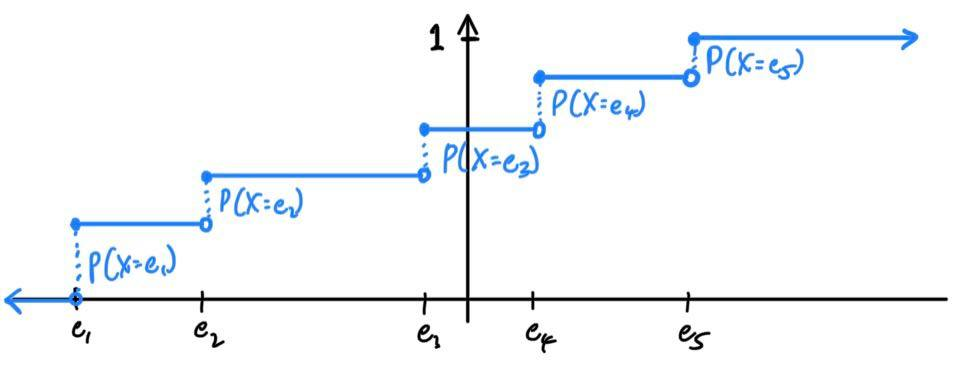
\includegraphics[scale=0.25]{img/Discrete_CDF.jpg}
\end{center}
If $E$ was countable, then it would have countably infinite discontinuities. Now we'll give some examples of discrete random variables, and in here we'll completely ignore the sample space $\Omega$, since once we have a random variable $X$, we can just work in $(\mathbb{R}, \mathcal{R}, \mathbb{P}_X)$. Remember that we will write $P(X = x)$ as shorthand for $\mathbb{P}_X (\{x\})$. 

\begin{definition}[Indicator/Bernoulli Random Variable]
Given $(\Omega, \mathcal{F}, \mathbb{P})$, let $A \in \mathcal{F}$ be an event. A useful random variable is the \textbf{indicator random variable} $1_A: \Omega \longrightarrow \mathbb{R}$ defined  
\[1_A (\omega) = \begin{cases} 1 & \text{ if } \omega \in A \\ 0 & \text{ if } \omega \not\in A \end{cases}\]
This is a random variable since the preimages of $\emptyset, \{0\}. \{1\}, \{0, 1\}$ are $\emptyset, A^c, A, \Omega$, which are all $\mathcal{F}$-measurable. Since the probability measure of $A$ is $\mathbb{P}(A) = p$, then $\mathbb{P}(A^c) = 1 - \mathbb{P}(A) = 1 - p$, and so we get the PMF 
\[p_{1_A} (x) = \begin{cases} 1 - p & \text{ if } x = 0 \\ p & \text{ if } x = 1 \end{cases}\]
The CDF of this function will look like a step function 
\[F_{1_A} (x) = \begin{cases} 0 & \text{ if } x < 0  \\ P(A^c) & \text{ if } 0 \leq x < 1 \\ 1 & \text{ if } 1 \leq x \end{cases}\]
\end{definition}

\begin{example}[Uniform Random Variable]
Given a finite set $E = \{e_i\}_{i=1}^n \subset \mathbb{R}$, we define the PMF as 
\[p_X (e_i) = \mathbb{P}(X = e_i) = \frac{1}{n} \; \forall i = 1, 2, \ldots n\]
which induces the probability measure $\mathbb{P}_X (B) = \sum_{x \in E \cap B} p_X (x)$. 
\end{example}

The Bernoulli RV leads to the geometric and binomial random variables. 

\begin{example}[Geometric Random Variable]
Given $E = \mathbb{N}$, we can define the PMF associated with random variable $X \sim \mathrm{Geometric}(p)$ as 
\[p_X (k) =\mathbb{P}(X = k) = (1 - p)^{k-1} p \text{ for } k \in \mathbb{N}, \; p \in [0, 1]\]
which induces the probability measure $\mathbb{P}_X (B) = \sum_{x \in E \cap B} p_X (x)$. We can interpret this as the number of times you have to (independently) toss a $p$-coin (probability of heads is $p$) until you get a heads. 
\end{example}

\begin{example}[Binomial Random Variable]
We let $E = \mathbb{N}_0$ and define the PMF associated with random variable $X \sim \mathrm{Binomial}(n, p)$ as 
\[p_X (k) = \mathbb{P}(X = k) = \binom{n}{k} p^k (1 - p)^{n - k} \text{ for } k \in E, p \in [0, 1]\]
We can interpret this as the number of heads occurring in a sequence of $n$ independent tosses of a $p$-coin. 
\end{example}

\begin{example}[Poisson Random Variable]
We let $E = \mathbb{N}_0$ and define the PMF of $X \sim \mathrm{Poisson}(\lambda)$ as 
\[p_X (k) = \frac{e^{-\lambda} \lambda^k}{k!} \text{ for } k \in E, \; \lambda > 0\]
\end{example}

A slight generalization of a discrete random variable is a simple random variable. Recall that the indicator random variable is a function $1_A: \Omega \rightarrow \mathbb{R}$ defined 
\[1_A (\omega) \coloneqq \begin{cases} 1 & \text{ if } \omega \in A \\
0 & \text{ if else } \end{cases}\]
As simple random variable generalizes this into multiple sets that form a partition of $\Omega$. It is analogous to a simple function, introduced in measure theory. 

\begin{definition}[Simple Random Variable]
Let $\{A_i\}_i$ form a partition of probability space $\Omega$. A \textbf{simple random variable} $X$ is a random variable of the form 
\[X (\omega) = \sum_{i} a_i 1_{A_i} (\omega)\]
that assigns value $a_i$ if the input $\omega \in A_i$. 
\end{definition}

Now, let's move on to continuous random variables. 

\begin{definition}[Absolutely Continuous Measures]
Let $\mu, \nu$ be measures defined on $(\Omega, \mathcal{F})$. We say that $\nu$ is \textbf{absolutely continuous} w.r.t. $\mu$ if for every $N \in \mathcal{F}$ s.t. $\mu(N) = 0$, we have $\nu(N) = 0$. 
\end{definition}

\begin{definition}[Continuous Random Variable]
A random variable $X$ is \textbf{continuous} if its induced measure $\mathbb{P}_X: (\mathbb{R}, \mathcal{R}) \rightarrow [0, 1]$ is absolutely continuous w.r.t. the Lebesgue measure $\lambda: (\mathbb{R}, \mathcal{R}) \rightarrow \mathbb{R}$, i.e. if for every Borel set $N$ of Lebesgue measure $0$, we have $\mathbb{P}_X (N) = 0$ also. 
\end{definition}

A common misconception is that a random variable $X$ is continuous if the induced measure on every singleton set in $\mathcal{B}(R)$ is $0$, i.e. $\mathbb{P}_X (\{x\}) = 0$ for all $x \in \mathbb{R}$. The definition above implies this since the Lebesgue measure of every singleton set is $0$. 

We introduce a theorem that is useful to know, but we won't prove it. 

\begin{theorem}[Radon-Nikodym Theorem (Special Case)]
Let $X$ be a continuous random variable. Then, there exists a nonnegative measurable function $f_X : \mathbb{R} \longrightarrow [0, \infty)$ s.t. for any $B \in \mathcal{R}$, we have 
\[\mathbb{P}_X (B) = \int_B f_X \, d\lambda\]
where the above is the Lebesgue integral. Note that we must define using the Lebesgue integral because Riemann integral is not compatible with any Borel set. $f_X$ is called the \textbf{probability density function}, aka \textbf{PDF}. Furthermore, we can get $f_X$ from $\mathbb{P}_X$ by taking the \textbf{Radon-Nikodym derivative} (which we will not define now)
\[f_X = \frac{d \mathbb{P}_X}{d \lambda}\]
which basically says that if we have a set of very small Lebesgue measure $d \lambda$ tending to $0$, then its probability measure $\mathbb{P}_X$ will also be very small, and the infinitesimal ratio of these two measures on an arbitrarily small set is $f_X$. Also, note that the integral does not change if the value of $f$ changes on sets of Lebesgue measure $0$, and so there is no unique PDF describing $\mathbb{P}_X$. It is unique up to sets of Lebesgue measure $0$, so when we refer to such a PDF $f_X$, we are really talking about an equivalence class of functions. 
\end{theorem}

This theorem guarantees the existence of some $f_X$ that completely describes the probability law $P_X$! Take a special case of when $B = (-\infty, x])$, and we can define the CDF as 
\[F_X (x) = P_X ((-\infty, x]) = \int_{(-\infty, x]} f_X \, d\lambda\]
If the set of integration is an interval (and the function is continuous a.e.), then the Lebesgue integral and Riemann integral coincides, and we get the familiar formula 
\[F_X (x) = \int_{-\infty}^x f_X (t)\,dt\]
and we can differentiate it to get back the PDF $f_X$ (or more accurately, some function that agrees with $f_X$ a.e.). We can show that the CDF of a continuous random variable $X$
\begin{enumerate}
    \item is absolutely continuous, and 
    \item is differentiable almost everywhere, which means that its PDF will be defined almost everywhere (and we can fill in the undefined points however we want). 
\end{enumerate}
Note that the PDF $f_X$ itself has no interpretation as a probability (indeed, we can change its value at a countable number of points to anything we want). It is only when we integrate it over some Borel set that gives us a probability. 

\begin{example}[Uniform Random Variable]
Let us define the uniform probability measure $P_X$ on $(\mathbb{R}, \mathcal{R})$ with the CDF 
\[F_X = \begin{cases} 0 & \text{ if } x < 0 \\
x & \text{ if } 0 \leq x \leq 1 \\
1 & \text{ if } 1 < x \end{cases}\]
It is differentiable almost everywhere except for at the two points $x = 0$ and $x = 1$. Therefore, the PDF $f_X$ is defined for all real numbers except $x = 0$ and $x = 1$. But it doesn't matter: we can assign any value $f_X$ we want on $0$ and $1$ since it won't affect the integral of it. In this example, we just set 
\[f_X = \begin{cases} 1 & \text{ if } 0 \leq x \leq 1 \\
0 & \text{ if else} \end{cases} \]
\end{example}

\begin{example}[Exponential Random Variable]
The exponential random variable has the following CDF: 
\[F_X (x) = \begin{cases} 1 - e^{-\lambda x} & \text{ if } x \geq 0 \\ 0 & \text{ if } x < 0 \end{cases} \text{ for } \lambda > 0\]
which is differentiable everywhere except at $x = 0$. Differentiating it (and assigning a convenient value at $x = 0$ $f(0) = \lambda$) gives the PDF 
\[f_X (x) = \begin{cases} \lambda e^{-\lambda x} & \text{ if } x \geq 0 \\ 0 & \text{ if else} \end{cases}\]
\end{example}

\begin{example}[Gaussian Random Variable]
The PDF is easier to specify for the Gaussian, so we define the Gaussian RV as having PDF 
\[f_X (x) = \frac{1}{\sigma \sqrt{2 \pi}} \exp \bigg( -\frac{(x - \mu)^2}{2 \sigma^2} \bigg) \text{ for } \mu \in \mathbb{R}, \sigma > 0\]
Note that this PDF decreases very quickly as we get further from $\mu$. The CDF cannot be written in closed form, and we call the CDF of the standard Gaussian the \textbf{error function}: 
\[\mathrm{Erf}(x) = F_X (x) = \int_{-\infty}^x \frac{1}{\sqrt{2 \pi}} e^{- t^2 / 2} \, dt\]
\end{example}

\begin{example}[Cauchy Random Variable (Standardized)]
The Cauchy random variable gives the PDF 
\[f_X (x) = \frac{1}{\pi} \frac{1}{1 + x^2} \text{ for } x \in \mathbb{R}\]
Integrating this gives the inverse tangent, which after scaling it down by $\pi$ satisfies the conditions of the CDF. Note that the Cauchy distribution falls off much more slowly around the mean (at a rate of $\frac{1}{1 + x^2}$, like a power law) than the Gaussian (which is even \textit{faster} than an exponential, it is at the rate of $e^{-x^2}$). If such a PDF falls off at a slow rate, like a power law, then this is called a \textit{heavy-tailed random variable}. 
\end{example}

\begin{example}[Gamma Random Variable]
The PDF associated with random variable $X \sim \mathrm{Gamma}(n, \lambda)$ is defined 
\[f_X(x) = \frac{\lambda^n x^{n-1}}{\Gamma(n)} e^{-\lambda x} \text{ for } x \geq 0\]
where $\Gamma$ is the gamma function, which is an extension of the factorial function to the domain of complex numbers. 
\[\Gamma(x) \coloneqq \int_{0}^\infty z^{x-1} e^{-z}\, dz, \;\;\;\;\; \text{Re}(x) > 0\]
\end{example}

\begin{example}[Beta Random Variable]
The PDF associated with random variable $X \sim \mathrm{Beta}(\alpha, \beta)$, for positive reals $\alpha, \beta$, is defined 
\[f_X (x) \equiv \frac{x^{\alpha-1} \,(1-x)^{\beta-1}}{B(\alpha, \beta)}, \text{ where } B(\alpha, \beta) \equiv \frac{\Gamma(\alpha) \Gamma(\beta)}{\Gamma(\alpha + \beta)}\]
and $\Gamma$ is the Gamma function. 
\end{example}

\begin{example}[Uniform RV defined on Cantor Set]
The cantor set $C \subset [0, 1]$ is defined by removing $(1/3, 2/3)$ from $[0, 1]$ and then removing the middle third from each interval that remains. We define the distribution on this set by defining its CDF: We set 
\begin{enumerate}
    \item $F(x) = 0$ for $x \leq 0$ and $F(x) = 1$ for $x \geq 1$. 
    \item $F(x) = 1/2$ for $x \in [1/3, 2/3]$, 
    \item $F(x) = 1/4$ for $x \in [1/9, 2/9]$ and $F(x) = 3/4$ for $x \in [7/9, 8/9]$, ... 
\end{enumerate}
and extend $F$ to all of $[0 ,1]$ using monotonicity. 
\end{example} 

\begin{example}[Dense Discontinuities]
Let $q_1, q_2, \ldots$ be an enumeration of the rationals. Let $\alpha_i > 0$ have $\sum_{i=1}^\infty \alpha_i = 1$, and let 
\[F(x) = \sum_{i=1}^\infty \alpha_i 1_{[q_i, \infty)} (x)\]
where $1_{[q_i, \infty)} (x) = 1$ if $x \in [q_i, \infty)$ and $0$ if otherwise. 
\end{example}

To summarize, once we have a random variable $X: \Omega \rightarrow \mathbb{R}$, we can throw away the sample space and work in $(\mathbb{R}, \mathcal{R}, \mathbb{P}_X)$ with the induced measure $\mathbb{P}_X$, which is known as the \textbf{probability distribution} of $X$.  
\begin{enumerate}
    \item If $X$ is discrete, then let there be some at most countable set $E = \{e_i\}$ where $P(E) = 1$. it turns out that $\mathbb{P}_X$ can be completely defined by a probability mass function $p_X : \mathbb{R} \rightarrow \mathbb{R}$ defined 
    \[p_X (x) = \mathbb{P}_X (\{x\}).\] 
    Given that we have this PMF , we can define $\mathbb{P}_X$ as such: Given any Borel $B \in \mathcal{R}$, 
    \[\mathbb{P}_X (B) = \sum_{x \in E \cap B} p_X (x)\]

    \item If $X$ is continuous, then the Radon-Nikodym Theorem asserts the existence of a nonnegative probability density function $f_X$ that completely describes the probability law $\mathbb{P}_X$. Given that we have this PDF, we can then define $\mathbb{P}_X$ as such: Given any Borel $B \in \mathcal{R}$, 
    \[\mathbb{P}_X (B) = \int_B f_X \, d\lambda\]
\end{enumerate}

\subsubsection{Space of Measurable Functions}

Now it turns out that the space of $\mathcal{F}$-measurable functions $X: \Omega \rightarrow \mathbb{R}$ forms a function space, which means that the set of all random variables on $\Omega$ forms a vector space. We formally show it here. 

\begin{lemma}
The set of all $\mathcal{F}$-measurable functions $X: (\Omega, \mathcal{F}) \rightarrow \mathbb{R}$ forms a vector space, denoted $L_\mathcal{F} (\Omega; \mathbb{R})$, or $L_\mathcal{F} (\Omega)$ for short. 
\end{lemma}
\begin{proof}

\end{proof}

Naturally, we can put the $L^p$-norm on this space, defined 
\[||X||_p \coloneqq \bigg( \int_\Omega |X|^p \, d\mathbb{P} \bigg)^{1/p}\]
Moreover, if $p = 2$, then we can put an inner product defined 
\[\langle X, Y \rangle = \bigg( \int_\Omega X Y \,d \mathbb{P} \bigg)^{1/2}\]

\begin{definition}
The Banach space of $\mathcal{F}$-measurable functions is denoted $L_\mathcal{F}^p (\Omega)$, and the Hilbert space is denoted $L_\mathcal{F}^2 (\Omega)$. 
\end{definition}

This means that if we have some probability space $(\Omega, \mathcal{F}, \mathbb{P})$ and  sub-$\sigma$-algebra $\mathcal{G} \subset \mathcal{F}$, then any $\mathcal{G}$-measurable function is also $\mathcal{F}$-measurable, since if the preimage of every $B \in \mathcal{R}$ is in $\mathcal{G}$, then it $B \in \mathcal{F}$. This immediately results in the following. 

\begin{theorem}
If $\mathcal{G}$ is a sub-$\sigma$-algebra of $\mathcal{F}$, then $L_\mathcal{G} (\Omega)$ is a subspace of $L_\mathcal{F} (\Omega)$. 
\end{theorem}

This means that as we get coarser and coarser random variables, the space in which these random variables live in get smaller and smaller, until we get to the constant random variables, which form a $1$-dimensional line in $L_\mathcal{F} (\Omega)$. The origin is simply the constant $0$ random variable. 

\subsection{Independence}

\begin{definition}[Independence of $2$ Events]
Given probability space $(\Omega, \mathcal{F}, \mathbb{\mathbb{P}})$, events $A, B \in \mathcal{F}$ are said to be \textbf{independent under $\mathbf{\mathbb{P}}$} if 
\[\mathbb{P}(A \cap B) = \mathbb{P}(A) \, \mathbb{P}(B)\]
This leads to the immediate property that if $\mathbb{P}(B) > 0$, with $A, B$ independent, then 
\[\mathbb{P}(A \mid B) = \mathbb{P}(A)\]
\end{definition}

Note that $A$ and $B$ may be independent under one measure, but not under another measure. The property that $\mathbb{P}(A \mid B) = \mathbb{P}(A)$ is \textit{not} the definition of independence, since it has the more restricting property that $\mathbb{P}(B) > 0$, so only refer to the definition that $\mathbb{P}(A \cap B) = \mathbb{P}(A) \, \mathbb{P}(B)$. This is the true definition of independent events that we should rely on, not the one that says that $A$ and $B$ are independent if "one does not affect the other." This old definition is misleading and false. For example, take the probability space $[0, 1]$, with Borel $\sigma$-algebra, and Lebesgue measure $\mathbb{P} = \lambda$, and let $A = \mathbb{Q}$ and $B = \mathbb{R} \setminus \mathbb{Q}$. Then, contradictory to our old definition, $A$ and $B$ are independent since $\mathbb{P}(A \cap B) = \mathbb{P}(A) \, \mathbb{P}(B) = 0$! By the definition, an event $A$ is independent of itself if $\mathbb{P}(A) = 0$ or $1$ (e.g. $A$ is rationals, irrationals, cantor set, $\emptyset$, $\Omega$, etc.). 

\begin{definition}[Independence of $n$ Events]
Given probability space $(\Omega, \mathcal{F}, \mathbb{P})$, 
\begin{enumerate}
    \item Let us have a finite collection of events $A_1, A_2, \ldots, A_n \in \mathcal{F}$. They are \textbf{independent} if for all nonempty $I_0 \subset \{1, 2, \ldots n\}$, 
    \[\mathbb{P} \bigg( \bigcap_{i \in I_0} A_i \bigg) = \prod_{i \in I_0} \mathbb{P}(A_i)\]
    Note that it is not enough to just prove that 
    \[\mathbb{P}(A_1 \cap \ldots \cap A_n) = \prod_{i=1}^n \mathbb{P}(A_i)\]
    We must verify this for all $2^n$ possible choices (to be precise, we don't need to prove for $I_0 = \emptyset$ and $I_0 = \{A_i\}$), so for $2^n - n - 1$ choices. 
    
    \item Let $\{A_i\}_{i \in I}$ be a collection of events indexed by a possibly uncountable $I$. They are independent if for all nonempty and finite $I_0 \subset I$, we have 
\[\mathbb{P} \bigg( \bigcap_{i \in I_0} A_i \bigg) = \prod_{i \in I_0} \mathbb{P}(A_i)\]
\end{enumerate}
\end{definition}

Now when we are trying to compare two $\sigma$-algebras, the measure defined for one may not even be defined on the other. To ensure that a measure is defined on both, it makes sense to take its $\sigma$-algebra and construct two sub-$\sigma$-algebras, which $\mu$ is guaranteed to be defined on. 

\begin{definition}[Independence of $\sigma$-Algebras]
Let us have probability space $(\Omega, \mathcal{F}, \mathbb{P})$. 
\begin{enumerate}
    \item Let $\mathcal{F}_1, \mathcal{F}_2$ be two sub-$\sigma$-algebras of $\mathcal{F}$. $\mathcal{F}_1$ and $\mathcal{F}_2$ are independent if for any $A_1 \in \mathcal{F}_1, A_2 \in \mathcal{F}_2$, $A_1$ and $A_2$ are independent. 
    \item Let $\{ \mathcal{F}_i\}_{i \in I}$ be an arbitrary collection of sub-$\sigma$-algebras of $\mathcal{F}$, indexed by possibly uncountable $I$. Then, they are independent if for any choices of $A_i \in \mathcal{F}_i$ for $i \in I$, $\{A_i\}_{i \in I}$ are independent events. 
\end{enumerate}
\end{definition}

\begin{definition}[Independent Random Variables]
Two random variables $X, Y$ are \textbf{independent} if $\sigma(X)$ and $\sigma(Y)$ are independent $\sigma$-algebras. That is, for any Borel sets $B_1, B_2 \in \mathcal{R}$, the events $X^{-1}(B_1)$ and $Y^{-1}(B_2)$ are independent: 
\[\mathbb{P}\big[ X^{-1}(B_1) \cap Y^{-1}(B_2) \big] = \mathbb{P}(X^{-1}(B_1)) \, \mathbb{P}(Y^{-1}(B_2))\]
or by abusing notation, 
\[\mathbb{P}(X \in B_1, Y \in B_2) = \mathbb{P}(X \in B_1) \, \mathbb{P}(Y \in B_2)\]
\end{definition}

If $X, Y$ are independent, then we can say something about the CDFs 
\[F_{X, Y} (x, y) = F_X (x) \, F_Y (y)\]
In fact, we can say something stronger. 

\begin{theorem}
$X$ and $Y$ are independent RVs if and only if 
\[F_{X, Y} (x, y) = F_X (x) \, F_Y (y)\]
\end{theorem}

Moving onto multiple variables, we can define that $X_1, X_2, \ldots, X_n$ are independent RVs if $\sigma(X_1), \ldots, \sigma(X_n)$ are independent $\sigma$-algebras. 

\subsection{Functions of Random Variables}

In many applications, it happens that we are interested not in the value of the random variable $X$, but a function of it. That is, given a probability space $(\Omega, \mathcal{F}, \mathbb{P})$, let us have a random variable $X: \Omega \rightarrow \mathbb{R}$. We can then define another function $f: \mathbb{R} \rightarrow \mathbb{R}$ and consider the potential random variable $f \circ X : \Omega \rightarrow \mathbb{R}$. We say potential because we don't know yet whether $f \circ X$ is measurable (i.e. the preimage of every Borel set in $\mathbb{R}$ is in $\mathcal{F}$). This condition suffices if $f$ itself is a measurable function, i.e. for every Borel set $B \in \mathcal{R}$, its preimage $f^{-1} (B)$ is Borel in $\mathbb{R}$, and by measurablility of $X$, its preimage under $X$ is $\mathcal{F}$-measurable, making $f \circ X$ a viable random variable. With this new random variable $f \circ X$, we would now like to answer the question: What is the probability law $\mathbb{P}_{f \circ X}$ of $\mathbb{R}$? 

This also works for joint random variables, which we will learn later. Given a joint random variable $(X_1, X_2, \ldots X_n): \Omega \rightarrow \mathbb{R}^n$, we can define a measurable function $f: \mathbb{R}^n \longrightarrow \mathbb{R}$ and define the scalar random variable $f \circ (X_1, \ldots X_n)$ on $\Omega$. But again, we want to find what the CDF of this composition. 

\subsubsection{Maximum/Minimum of Random Variables}

Let $X_1, X_2, \ldots, X_n$ be random variables of $(\Omega, \mathcal{F}, \mathbb{P})$ with joint CDF $F_{X_1 \ldots X_n} (x_1, \ldots, x_n)$. Let $Y_n = \min (X_1, \ldots, X_n)$ and $Z_n = \max(X_1, \ldots, X_n)$. Note that $Y_n$ and $Z_n$ are also functions of $\Omega$ to $\mathbb{R}$. To prove that they are random variables, we just have to prove that $\min$ and $\max$ are measurable functions from $\mathbb{R}^n$ to $\mathbb{R}$, which we can do by proving that the preimage of all semi-infinite interval $(-\infty, x]$ are Borel in $\mathbb{R}^n$. 
\begin{enumerate}
    \item The preimage of $(-\infty, x]$ under $\max$ is just the set of all $n$-vectors whose max is less than $x$, which is just the semi-infinite cuboid $(-\infty, x]^n \subset \mathbb{R}^n$, which is Borel in $\mathbb{R}^n$. 
    \item The preimage of $(-\infty, x]$ under $\min$ is the set of all $n$-vectors whose min is less than $x$, i.e. at least one element must be less than $x$. But this is just the complement of all vectors that have elements all greater than $x$, which is $\mathbb{R}^n \setminus (x, +\infty)^n \subset \mathbb{R}^n$, which is Borel in $\mathbb{R}^n$. 
\end{enumerate}
Now we must determine the CDF of $Y_n$ and $Z_n$. 
\begin{enumerate}
    \item We have 
    \begin{align*}
        F_{Z_n} (z) & = \mathbb{P}(\{ \omega \mid Z_n (\omega) \leq z \}) \\
        & = \mathbb{P}(\{ \omega \mid X_1 (\omega) \leq z, \ldots, X_n (\omega) \leq z\}) \\
        & = F_{X_1 \ldots X_n} (z, \ldots, z)
    \end{align*}
    where the last equality is describes simply the joint CDF of the joint distribution $(X_1, \ldots, X_n)$. If we assume independence of $X_i$'s, it simplifies out to 
    \[\prod_{i} F_{X_i} (z)\]
    and if iid, then we have $[F_{X} (z) ]^n$, where $X$ is the common distribution. 
    \item For $Y_n$, we work with complements again and have 
    \begin{align*}
        F_{Y_n} (y) & = \mathbb{P}(\{ \omega \mid Y_n (\omega) \leq y \}) \\ 
        & = 1 - \mathbb{P}(\{ \omega \mid Y_n (\omega) > y \}) \\
        & = 1 - \mathbb{P}(\{ \omega \mid X_1 (\omega) > y, \ldots X_n (\omega) > y \}) \\
    \end{align*}
    where $\mathbb{P}(\{ \omega \mid X_1 (\omega) > y, \ldots X_n > y \})$ can be calculated from the joint distribution. If we assume independence of $X_i$, it simplifies out to 
    \[1 - \prod_{i} \mathbb{P}(\{\omega \mid X_i(\omega) > y \}) = 1 - \prod_{i} \big( 1 - F_{X_i} (y) \big)\]
    and if iid, then we have $1 - [1 - F_{X} (y)]^n$. 
\end{enumerate}

\begin{example}[Uniforms]
Let $X_1, X_2$ be iid distributed as $\mathrm{Uniform}[0, 1]$, and let $Z = \max(X_1, X_2)$ with $Y = \min(X_1, X_2)$, i.e. $Z$ is the greater of the two and $Y$ is the lesser. We would expect the PDF of $Z$ to have more mass towards $1$ and the PDF of $Y$ to have more mass towards $0$. Our common CDF is 
\[F_{X} (x) = \begin{cases} 0 & \text{ if } x < 0 \\
x & \text{ if } 0 \leq x \leq 1 \\
1 & \text{ if } 1 < x \end{cases}\]
Let's calculate the CDF of $Z$. 
\begin{align*}
    F_{Z} (z) & = \mathbb{P}(\{\omega \mid Z(\omega) \leq z\}) \\
    & = \mathbb{P}(\{ \omega \mid X_1 (\omega) \leq z, X_2 (\omega) \leq z\}) \\
    & = F_{X_1, X_2} (z, z) \\
    & = [F_{X} (z)]^2 = \begin{cases} 0 & \text{ if } x < 0 \\
x^2 & \text{ if } x \in [0, 1] \\
1 & \text{ if } 1 < x \end{cases}
\end{align*}
This CDF is differentiable everywhere except the two points $0$ and $1$, so we can get the PDF to be $f_Z (z) = 2 z$ for $z \in (0, 1)$ and $0$ otherwise. For the values of $f_Z$ at $0$ and $1$, we can fill it in with anything we want (since the measure of these sets are $0$), so we will just defined $f_Z (0) = 0$ and $f_Z(1) = 2$, getting 
\[f_Z (z) = \begin{cases} 2 z & \text{ if } z \in [0, 1] \\
0 & \text{ if else} \end{cases}\]
Let's calculate the CDF of $Y$. 
\begin{align*}
    F_{Y} (y) & = \mathbb{P}(\{ \omega \mid Y(\omega) \leq y\}) \\
    & = 1 - \mathbb{P}(\{ \omega \mid Y(\omega) > y\}) \\
    & = 1 - \mathbb{P}(\{\omega \mid X_1 (\omega) > y, X_2 (\omega) > y \}) \\
    & = 1 - \mathbb{P}(\{\omega \mid X_1 (\omega) > y\}) \, \mathbb{P}(\{ X_2 (\omega) > y \}) \\ 
    & = 1 - [1 - F_X (y)]^2 = \begin{cases} 0 & \text{ if } y < 0 \\
    1 - (1 - y)^2 & \text{ if } y \in [0, 1] \\
    1 & \text{ if } y > 1 \end{cases} 
\end{align*}
and differentiating it (with setting any values of the PDF at the nondifferentiable points $0$ and $1$) gives 
\[f_Y (y) = \begin{cases} 2 - 2y & \text{ if } y \in [0, 1] \\
0 & \text{ if else} \end{cases} \]
\end{example}

\begin{example}[Exponentials]
Let $X_1, X_2, \ldots, X_n$ be independent exponential random variables with parameters $\lambda_1, \ldots, \lambda_n$, respectively (not identical!). Then, for each $X_i$, its CDF is 
\[F_{X_i} (x) = 1 - e^{-\lambda_i x} \text{ for } x \geq 0\]
and let $Y = \min(X_1, \ldots, X_n)$. Then, we have 
\begin{align*}
    F_Y (y) & = 1 - \prod_{i=1}^n [ 1 - F_{X_i} (y)] \\
    & = 1 - \prod_{i=1}^n e^{-\lambda_i x} \\
    & = 1 - e^{- ( \sum_{i=1}^n \lambda_i ) x}
\end{align*}
which is the CDF of an exponential distribution. So, 
\[Y \sim \mathrm{Exponential}(\lambda_1 + \ldots + \lambda_n)\]
This is nice, since the minimum of a bunch of exponentials is an exponential. However, this is not the case for the maximum. 
\end{example}

This has nice practical applications. For example, recall the memoryless property of the exponential, which nicely models radioactive decay. If we have $n$ elements each decaying at some $\mathrm{Exponential}(\lambda_i)$ rate, then we can model the time at which the first alpha particle will emit amongst all $n$ elements will also be an exponential. These processes where the inter-emission times are exponentials are called Poisson process, which we will discuss later. 


\begin{definition}[Order Statistic]
Let $X_1, X_2, ..., X_n$ be a finite collection of independent, identically distributed random variables. Suppose that they are continuously distributed with density $f$ and CDF $F$. Define the random variable $X_{(k)}$ to be the $k$th ranked value, called the \textbf{$k$th order statistic}. This means that 
\[X_{(1)} = \min\{X_1, X_2, ..., X_n\}, \;\; X_{(n)} = \max\{X_1, X_2, ..., X_n\}\]
and in general, for any $k \in \{1, 2, ..., n\}$, 
\[X_{(k)} = X_j \text{ if } \sum_{l=1}^n \mathbb{I}_{X_l < X_j} = k - 1\]
which means that exactly $k-1$ of the values of $X_l$ are less than $X_j$. Since $F$ is continuous, 
\[X_{(1)} < X_{(2)} < ... < X_{(n)}\]
holds with probability $1$. This leads us to define the random variable $X_{(k)}$ representing the $k$th order statistic.
\[f_{(k)} (y) = \begin{cases} 
n \, \binom{n-1}{k-1} y^{k-1} (1-y)^{n-k} & y \in (0, 1) \\
0 & y \not\in (0,1)
\end{cases}\]
That is, $X_{(k)}$ has the Beta$(k, n-k_1)$ distribution. 
\end{definition}


\subsubsection{Sums of Random Variables}

Now given two random variables $X, Y: \Omega \rightarrow \mathbb{R}$ that each push their own probability laws $\mathbb{P}_X, \mathbb{P}_Y$ onto $\mathbb{R}$, their sum $Z = X + Y$ is also a random variable that pushes its own probability law $\mathbb{P}_Z$. We must actually prove that $Z$ is a random variable, which we can do by proving that the preimage of every $(-\infty, x]$ is $\mathcal{F}$-measurable. Equivalently (by complementation), we must prove that the preimage of every $(x, +\infty)$ (that is, all sets of form $\{ \omega \mid Z(\omega) > z\}$) is $\mathcal{F}$-measurable. Now we can write $z$ as the sum of two numbers $z = q + (z - q)$, where $q \in \mathbb{R}$, and say that 
\[\{ \omega \mid Z(\omega) > z\} = \bigcup_{q \in \mathbb{R}} \{ \omega \mid X (\omega) > q , \; Y(\omega) > z - q\}\]
But using the fact that $\mathbb{Q}$ is dense in $\mathbb{R}$, we can turn this from an uncountable union to a countable union and say 
\begin{align*}
    \{ \omega \mid Z(\omega) > z\} & = \bigcup_{q \in \mathbb{Q}} \{ \omega \mid X (\omega) > q , \; Y(\omega) > z - q\} \\
    & = \bigcup_{q \in \mathbb{Q}} \big( \{\omega \mid X(\omega) > q\} \cap \{ \omega \mid Y(\omega) > z - q\} \big) 
\end{align*}
and since I have a countable union of (an intersection of) these $\mathcal{F}$-measurable sets, $\{ \omega \mid Z(\omega) > z\}$ is $\mathcal{F}$-measurable, and we are done. This equation above even gives us a hint of how to compute the CDF of $Z$. 

\begin{theorem}
Given random variables $X_1, X_2, \ldots, X_n$ of probability space $(\Omega, \mathcal{F}, \mathbb{P})$, 
\begin{enumerate}
    \item $X_1 + \ldots + X_n$ is a random variable.
    \item $X_1 \cdot \ldots \cdot X_n$ is a random variable. 
\end{enumerate}
\end{theorem}

For simplicity, we will only consider jointly discrete or jointly continuous random variables. The probability law $\mathbb{P}_Z$ can be confusing to define, since given some Borel set $B \in \mathcal{R}$, we must now look at the preimage under the \textit{sum} $X + Y$. A simpler way to approach this is to consider the joint distribution $X, Y$ and look at its distribution. This is especially simple to consider for discrete random variables. 

\begin{definition}[Sums of Discrete Random Variables]
Take two discrete random variables $X, Y$ with their joint PMF $p_{X, Y} (x, y)$ and their sum $Z = X + Y$. We can see that the PMF of $Z$ is 
\[p_Z (z) = \sum_{(x, y) \,:\, x + y = z} p_{X, Y} (x, y) = \sum_{x \in \mathcal{X}} p_{X, Y} (x, z - x)\]
which by abuse of notation, we denote
\[\mathbb{P}(Z = z) = \sum_{x \in \mathcal{X}} \mathbb{P}(X = x, Y = z - x) \]
The CDF is very simple, since we just have to sum over all $(x, y)$ such that their sum is less than $z$: 
\[F_Z (z) = \sum_{(x, y) \,:\, x + y \leq z} p_{X, Y} (x, y)\]
which by abuse of notation, we write 
\[\mathbb{P}(Z \leq z) = \sum_{(x, y) \,:\, x + y \leq z} \mathbb{P}(X = x, Y = y) \]
If $X$ and $Y$ are independent, then their joint distribution is the product of their singular distributions, and so we have 
\[p_Z (z) = \sum_x p_X (x) \, p_Y (z - x) \coloneqq p_X \ast p_Y\]
where $p_Z = p_X \ast p_Y$ is called the convolution of $p_X$ and $p_Y$. By abuse of notation, 
\[\mathbb{P}(Z = z) = \sum_{x \in \mathcal{X}} \mathbb{P}(X = x) \, \mathbb{P}(Y = z - x) \]
\end{definition}

\begin{example}[Sums of Poisson RVs]
Let $X_1$ and $X_2$ be independent Poisson random variables with parameters $\lambda_1, \lambda_2 > 0$, and let $Z = X_1 + X_2$. The PMF of each $X_i$ is 
\[p_{X_i} (k) = \frac{e^{-\lambda_i} \lambda_i^k}{k!} \text{ for } k \in \mathbb{Z}\]
and taking the convolution gives the PMF of $Z$: 
\begin{align*}
    p_Z (z) & = (p_{X_1} \ast p_{X_2}) (z) \\
    & = \sum_{k=-\infty}^{+\infty} \frac{e^{-\lambda_1} \lambda_1^k}{k!} \cdot \frac{e^{-\lambda_2} \lambda_2^{z - k}}{(z - k)!} \\
    & = \sum_{k=0}^{z} \frac{e^{-\lambda_1} \lambda_1^k}{k!} \cdot \frac{e^{-\lambda_2} \lambda_2^{z - k}}{(z - k)!} \\ 
    & = \frac{e^{-(\lambda_1 + \lambda_2)}}{z!} \sum_{k=0}^z \binom{z}{k} \lambda_1^k \lambda_2^{z - k} \\
    & = \frac{e^{-(\lambda_1 + \lambda_2)} (\lambda_1 + \lambda_2)^z}{z!} 
\end{align*}
for $z \in \mathbb{N}_0$, which is the PMF of another Poisson. So, $Z \sim \mathrm{Poisson}(\lambda_1 + \lambda_2)$. 
\end{example}

This has a nice visualization, since the joint distribution of $X$ and $Y$ over $\mathbb{R}^2$ is being "summed up/integrated" over the diagonals of $\mathbb{R}^2$, i.e. the lines where $x + y = z$ for some $z$, sort of like marginalizing over these diagonals. This creates a new "diagonally marginal distribution" $Z$. 

\begin{definition}[Sums of Continuous Random Variables]
Take two continuous random variables $X, Y$ with their joint PDF $f_{X, Y} (x, y)$ and their sum $Z = X + Y$. To calculate the CDF, we must basically integrate the joint PDF over the borel set $\{(x, y) \in \mathbb{R}^2 \mid x + y \leq z\}$. 
\begin{align*}
    \mathbb{P}(Z \leq z) = F_Z (z) & = \int_{(x, y) \,:\, x + y \leq z} f_{X, Y} (x, y) \,dy\,dx \\
    & = \int_{-\infty}^{+\infty} \int_{-\infty}^{z - x} f(x, y) \,dy \,dx
\end{align*}
We can see that the PDF of $Z$ is 
\[f_{Z} (z) = \int_{\mathbb{R}} f_{X, Y} (x, z - x) \, dx\]
If $X$ and $Y$ are independent, then 
\[f_{Z} (z) = \int_{\mathbb{R}} f_{X} (x) \, f_Y (z - x) \,dx \coloneqq f_X \ast f_Y\]
where $f_Z = f_X \ast f_Y$ is the convolution of $f_X$ and $f_Y$. 
\end{definition}

\begin{definition}[Convolution]
Given two functions $f, g: \mathbb{R} \longrightarrow \mathbb{R}$, the \textbf{convolution} of $f$ and $g$ is a new function $f \ast g$ defined  
\[(f \ast g) (t) \coloneqq \int_\mathbb{R} f(t)\, g(t - \tau) \, d \tau\]
\end{definition}

Usually, when we take convolutions, it is not pretty and even for nice distributions like two Gaussians, convolving them is quite complicated. What we can do is transform them (using Laplace, Fourier, etc.) to make calculations easier and more elegant. 

\begin{example}
Let $X_1$ and $X_2$ be independent exponential with parameters $\lambda_1, \lambda_2$, with individual PDFs $f_{X_i} (x) = \lambda_i e^{-\lambda_i x}$ for $x \geq 0$. Let $Z = X_1 + X_2$. Then, 
\begin{align*}
    f_Z (z) = (f_{X_1} \ast f_{X_2})(z) & = \int_{-\infty}^\infty \lambda_1 e^{-\lambda_1 x} \, \lambda_2 e^{-\lambda_2 (z -x)} \, dx \\
    & = \int_{0}^z \lambda_1 e^{-\lambda_1 x} \, \lambda_2 e^{-\lambda_2 (z -x)} \, dx \\ 
    & = \lambda_1 \lambda_2 e^{-\lambda_2 z} \int_0^z e^{(\lambda_2 - \lambda_1) x}\,dx \\
    & = \begin{cases} \frac{\lambda_1 \lambda_2}{\lambda_2 - \lambda_1} \big( e^{-\lambda_1 z} - e^{-\lambda-2 z} \big) & \text{ if } \lambda_1 \neq \lambda_2 \\
    \lambda^2 z e^{-\lambda z} & \text{ if } \lambda_1 = \lambda_2 = \lambda \end{cases} 
\end{align*}
The distribution for when $\mu_1 = \mu_2$ is called the Erlang distribution, which has many applications, but the other case is an ugly form and not studied very well. 
\end{example}

\begin{theorem}[Sums of Discrete Variables]
Assume that $X$ and $Y$ are independent. 
\begin{enumerate}
    \item $X \sim$ Binomial$(n, p)$, $Y \sim$ Binomial$(m, p)$ $\implies X + Y \sim$ Binomial$(n + m, p)$. 
    \item $X \sim$ Poisson$(\lambda)$, $Y \sim$ Poisson$(\gamma)$ $\implies X + Y \sim$ Poisson$(\lambda + \gamma)$. 
    \item If $X_1, ..., X_n$ are Geometric$(p)$, then $X_1 + ... + X_n$ is NB$(n, p)$. 
\end{enumerate}
\end{theorem}

\begin{theorem}[Sums of Densities]
Assume that $X$ and $Y$ are independent. 
\begin{enumerate}
    \item $X \sim$ Normal$(\mu_1, \sigma_1^2)$, $Y \sim$ Normal$(\mu_2, \sigma_2^2)$ $\implies X + Y \sim$ Normal $(\mu_1 + \mu_2, \sigma_1^2 + \sigma_2^2)$. 
    \item If $X_1, X_2, ..., X_n$ are Exponential$(\lambda)$, then $X_1 + ... + X_n \sim$ Gamma$(n, \lambda)$.
    \item $X \sim$ Gamma$(n, \lambda)$, $Y \sim$ Gamma$(m, \lambda)$ $\implies X + Y \sim$ Gamma$(n + m, \lambda)$. 
    \item $X \sim$ Gamma $(n, \lambda)$, $Y \sim$ Exponential $(\lambda)$ $\implies X + Y \sim$ Gamma$(n+1, \lambda)$. 
\end{enumerate}
\end{theorem}

\subsubsection{Sum of Random Number of Random Variables}

Now we consider a random variable where the number of terms we are summing is a random variable. Let $\{X_i\}_i$ be a countable sequence of independent random variables with CDF $F_{X_i}$. Let $N$ be a positive integer-valued random variable with PMF $p_N(n) = \mathbb{P}(N = n)$. Assume that $N$ is independent of $X_i$'s. Now, consider the function 
\[S_N \coloneqq \sum_{i=1}^N X_i\]
To interpret this, consider the sample space $\Omega$. We have all $X_i$'s and $N$ defined on the same $\Omega$. Once $\omega \in \Omega$ realizes, the $\{X_i\}$'s will realize as a sequence of numbers, and $N$ will realize as a positive integer. We simply sum them up according to the rule $S_N$, and by this definition, $S_N$ is a real-valued function on $\Omega$. We first have to prove that $S_N$ is a random variable (since we only know that a \textit{fixed} sum of random variables is a random variable), and then we must find the CDF of $S_N$ $\mathbb{P}(S_N \leq x)$. 

First, note that the realization of $N$ partitions the sample space as 
\[\Omega = \bigsqcup_{n = 1}^\infty \{\omega \mid N(\omega) = n\}\]
Once I have this partition, I can invoke the partition rule and write 
\begin{align*}
    \mathbb{P}(S_N \leq x) & = \sum_{k=1}^\infty \mathbb{P}(S_N \leq x \mid N = k) \, \mathbb{P}(N = k) \\
    & = \sum_{k=1}^\infty \mathbb{P}(S_k \leq x \mid N = k) \, \mathbb{P}(N = k) & (\text{conditioned on } N = k) \\
    & = \sum_{k=1}^\infty \mathbb{P}(S_k \leq x) \, \mathbb{P}(N = k) & (N \text{ is indep. of } X_i \text{s})
\end{align*}
where $\mathbb{P}(N = k)$ is known since we know the PMF of $N$, and the CDFs $\mathbb{P}(S_k \leq x)$ can be computed by computing the deterministic sums and computing their CDF. 

\begin{example}
Let $X_i$'s be iid $\mathrm{Exponential}(\lambda)$, and $N \sim \mathrm{Geometric}(p)$. We know that the deterministic sum of iid exponentials gives an Erlang. So, $S_N = \sum_{i=1}^N X_i$, and its CDF is 
\[\mathbb{P}(S_N \leq x) = \sum_{k=1}^\infty \mathbb{P}(S_k \leq x) \, \mathbb{P}(N = k)\]
where $\mathbb{P}(N = k) = (1 - p)^{k - 1} p$. The PDF of the Erlang is 
\[p_{S_k} (x) = \frac{\lambda^n x^{n-1}}{(n - 1)!} e^{-\lambda x}\]
and doing the brute force calculations gives a clean $S_N \sim \mathrm{Exponential}(\lambda p)$. 
\end{example}

\subsubsection{General Transformations of Random Variables}

Now we will look at more general transformations that are not just minimum, maximum, deterministic sums, or random sums. Let us have a probability space $(\Omega, \mathcal{F}, \mathbb{P})$, a random variable $X: \Omega \rightarrow \mathbb{R}$, and a measurable function $f: \mathbb{R} \rightarrow \mathbb{R}$. Now given that we know the CDF (and therefore distribution) of $X$, we want to find the CDF of random variable $Y = f(X) = f \circ X$ (which we have established as a random variable already due to measurability of $f$): $F_Y (y) = \mathbb{P}(Y \leq y)$, which is just $\mathbb{P}_Y ((-\infty, y])$ (where $\mathbb{P}_Y$ is the probability law on $Y$). But rather than trying to take the preimage of the entire composite random variable $Y$ and calculating $\mathbb{P}\big( Y^{-1}((-\infty, y]) \big)$ under the probability on $\mathcal{F}$, let's just take the preimage one step at a time. Note that $f^{-1} \big( (-\infty, y] \big) = \{x \in \mathbb{R} \mid f(x) \leq y\}$. We can then write the CDF of $Y$ in terms of the probability law of $X$: 
\begin{align*}
    F_Y (y) & = \mathbb{P}_X \big( f^{-1} ((-\infty, y]) \big) \\
    & = \mathbb{P}_X \big( \{x \in \mathbb{R} \mid f(x) \leq y\} \big) \\
    & = \mathbb{P} \big( X^{-1} \circ f^{-1} ((-\infty, y]) \big) 
\end{align*}
Depending on how complicated $f$ is, this may be easy or not, but conceptually, this is no problem. But theoretically, this is as far as we can go. Let's move onto some examples. 

\begin{example}[Chi-Squared Distribution]
Let $X \sim \mathcal{N}(0, 1)$ and $Y = f(X) = X^2$. Note that $X$ takes values in $(-\infty, +\infty)$ and $Y$ in $[0, +\infty)$. Then, we can write 
\begin{align*}
    F_Y (y) & = \mathbb{P}(Y \leq y) \\ 
    & = \mathbb{P}_Y ( (-\infty, y]) \\
    & = \mathbb{P}_Y (  [0, y]) & (\text{range of } Y) \\
    & = \mathbb{P}_X ( f^{-1} ([0, y]) ) & (\text{work in prob. law of } X) \\
    & = \mathbb{P}_X ( [-\sqrt{y}, \sqrt{y}] ) \\
    & = \int_{-\sqrt{y}}^{\sqrt{y}} f_X (x) \,dx 
\end{align*}
Rewriting this in our abuse of notation notation, we have 
\begin{align*}
    F_Y (y) & = \mathbb{P}(Y \leq y) \\
    & = \mathbb{P}(X^2 \leq y) \\
    & = \mathbb{P}( -\sqrt{y} \leq X \leq \sqrt{y}) \\
    & = 2 \mathbb{P}(0 \leq X \leq \sqrt{y}) & (\text{Symmetry of Gaussian})\\
    & = \frac{2}{\sqrt{2} \pi} \int_0^{\sqrt{y}} e^{-x^2 / 2} \,dx 
\end{align*}
and this is clearly differentiable, since it is written like an integral. Doing so gives the PDF
\[f_Y (y) = \frac{1}{\sqrt{2 \pi y}} e^{-y/2} \text{ for } y \geq 0\]
This describes the PDF of a \textbf{Chi-Squared} distribution. 
\end{example}

\begin{example}[Log-Normal Distribution]
Let $X \sim \mathcal{N}(0, 1)$ and $Y = f(X) = e^X$. Note that the range of $f$ is $(0, +\infty)$. So, 
\begin{align*}
    F_Y (y) & = \mathbb{P}(Y \leq y) \\
    & = \mathbb{P}_Y ((-\infty, y]) \\
    & = \mathbb{P}_Y ( (0, y]) \\ 
    & = \mathbb{P}_X ( f^{-1} ((0, y]) ) \\
    & = \mathbb{P}_X ( (-\infty, \ln{y}] ) \\
    & = \int_{-\infty}^{\ln{y}} f_X (x)\,dx 
\end{align*}
Rewriting this in our abuse of notation notation, we have 
\begin{align*}
    F_Y (y) & = \mathbb{P}(e^X \leq y) \\
    & = \mathbb{P}(X \leq \ln(y)) \\ 
    & = \int_{-\infty}^{\ln(y)} \frac{1}{\sqrt{2} \pi} e^{-x^2/ 2} \,dx 
\end{align*}
We can differentiate this to get 
\[f_Y (y) = \frac{1}{y \sqrt{2 \pi}} e^{-\frac{(ln{y})^2}{2}} \text{ for } y \geq 0\]
This describes the PDF of a \textbf{log-normal} distribution. 
\end{example}

We now show a more specific formula under more specific assumptions about the transformation. Suppose $X$ is a \textit{continuous} random variable with density $f_X$ and $g: \mathbb{R} \rightarrow \mathbb{R}$ a monotonic differentiable function. Then, the CDF of the random variable $Y = g(X)$ can be written in the probability law of $X$, which can then by written as an integral by invoking the Radon-Nikodym theorem: 
\begin{align*}
    \mathbb{P}(Y \leq y) & = \mathbb{P}_X (f^{-1} ((-\infty, y]) \\
    & = \int_{x \,:\, g(x) \leq y} f_X (x) \,dx
\end{align*}
Note that we can now talk about the actual inverse $g^{-1}$ since differentaible and monotonic implies invertibility. 
\begin{enumerate}
    \item Assuming $g$ is monotonically increasing, we can use the change of variables $x = g^{-1} (t)$ and $g(x) = t \implies g^\prime (x) \,dx = dt$ to get the above integral as 
    \[\int_{-\infty}^{g^{-1} (y)} f_X (x) \,dx = \int_{-\infty}^t \frac{f_X \big( g^{-1} (t) \big)}{g^\prime \big( g^{-1} (t)\big)} \,dt \]
    but since this is simply the CDF of $Y$, the PDF must equal 
    \[f_Y (y) = \frac{f_X (g^{-1} (y) )}{g^\prime (g^{-1} (t))}\]
    \item If $g$ is monotonically decreasing, we get 
    \[f_Y (y) = \frac{f_X (g^{-1} (y) )}{- g^\prime (g^{-1} (t))}\]
\end{enumerate}
In general, we can consider both cases by putting an absolute value 
\[f_Y (y) = \frac{f_X (g^{-1} (y) )}{|g^\prime (g^{-1} (t))|}\]
and $g^\prime (g^\prime (y))$ is the Jacobian, the same one that we use when we perform a change of variables in integration. 

\begin{example}[Log-Normal Revisited]
Given $X \sim \mathcal{N}(0, 1)$ and $Y = e^X$ (which is monotonically increasing), we can simply plug in the formula to get the PDF: 
\[f_Y (y) = \frac{f_X (g^{-1} (y) )}{|g^\prime (g^{-1} (t))|} = \frac{f_X (\ln{y}) }{ | e^{\ln{y}} |} = \frac{1}{\sqrt{2 \pi} y} e^{-(\ln{y})^2 / 2}\]
for $y > 0$. This domain is important since $\ln{y}$ is only defined for $y > 0$. 
\end{example}

\begin{example}
Given $X \sim \mathcal{N}(0, 1)$ and $Y = f(X) = X^2$, we cannot use the formula since $f$ is not monotonic on the range of $X$, which is $(-\infty, +\infty)$.  
\end{example}

\begin{example}
Given $X \sim \mathrm{Exponential}(\lambda)$ and $Y = f(X) = X^2$, it may seem like the formula is not applicable here, but $f$ \textit{is} monotonic on the range of $X$, which is $[0, + \infty)$. 
\end{example}

However, there is much less chance of error by deriving using first principles, so I would recommend using it always rather than these formulas. 

Let's do the $n$-dimensional version of this. Given random variables $X_1, X_2, \ldots, X_n$ iid random variables with joint density $f_{X_1 \ldots X_n} (x_1, \ldots, x_n)$, we define the transformation $g: \mathbb{R}^n \rightarrow \mathbb{R}^n$ as 
\[\begin{bmatrix} Y_1 \\ \vdots \\ Y_N \end{bmatrix} = \begin{bmatrix} g_1 (X_1) \\ \vdots \\ g_n (X_N) \end{bmatrix}\]
Then, the PDF of $Y$ will be 
\begin{align*}
    f_{Y_1 \ldots Y_n} (y_1, \ldots, y_n) & = f_{X_1 \ldots X_n} \big( \mathbf{g}^{-1} (\mathbf{y}) \big) \cdot | \mathbf{J}(\mathbf{y})| \\
    & = f_{X_1 \ldots X_n} \big( g_1^{-1}(y_1), \ldots, g_n^{-1} (y_n) \big) \cdot | \mathbf{J}(\mathbf{y})| \\
\end{align*}
where 
\[\mathbf{J}(y) = \mathrm{det}\begin{pmatrix} 
\frac{\partial x_1}{\partial y_1} & \ldots & \frac{\partial x_n}{\partial y_1} \\
\vdots & \ddots & \vdots \\ 
\frac{\partial x_1}{\partial y_n} & \ldots & \frac{\partial x_n}{\partial y_n} \end{pmatrix}\]


\section{Integration}

\subsection{Construction and Properties}

\subsubsection{Simple Functions}

Remember that Riemann integration is characterized by the approximation of step functions, which are the "building blocks" of Riemann integrable functions. To define the Lebesgue integral, we will consider a generalization of step functions called \textit{simple functions}. A function will be Lebesgue integrable if it can be approximated by these simple functions in some appropriate way. 

\begin{definition}[Simple Functions]
For $A \subset X$ (any subset, not just in some $\sigma$-algebra), the \textbf{characteristic}, or \textbf{indicator} \textbf{function} of $A$ is the function $1_A : X \longrightarrow \mathbb{R}$ defined 
\[1_A (x) = \begin{cases} 1 & \text{ if } x \in A \\ 0 & \text{ if else} \end{cases}\]
A function $\phi: \mathbb{R} \longrightarrow \mathbb{R}$ is called a \textbf{simple function} if it is a finite linear combination of characteristic functions. 
\[\phi = \sum_{i=1}^n a_i 1_{A_i}\]
\end{definition}

\begin{lemma}[Measurability on Simple Functions]
Now, let $(X, \mathcal{A})$ be a measurable space. Then, 
\[\phi = \sum_{i=1}^n a_i 1_{A_i} : (X, \mathcal{A}) \longrightarrow \mathbb{R}\]
is measurable if all $A_i$ are measurable, i.e. $A_i \in \mathcal{A}$ for all $i$. 
\end{lemma}
\begin{proof}
Let $T$ be an open set in $\mathbb{R}$. Then, for characteristic function $1_A$, 
\[1_A^{-1} (T) = \begin{cases} 
\emptyset & \text{ if } 0, 1 \not\in T \\
A & \text{ if } 1 \in T, 0 \not\in T \\
X \setminus A & \text{ if } 0 \in T, 1 \not\in T \\
X & \text{ if } 0, 1 \in T
\end{cases}\]
and so $1_A$ must be measurable if $A \in \mathcal{A}$ (which also by definition implies that $A^c = X \setminus A \in \mathcal{A}$). If $1_{A_i}$ is measurable, then the linear combination of measurable functions is also measurable. 
\end{proof}

Also observe that the coefficients need not be unique, since we can write 
\[1 \cdot 1_{[0, 1]} + 1 \cdot 1_{[0.5, 1]} = 1 \cdot 1_{[0, 0.5]} + 2 \cdot 1_{[0.5, 1]}\]
If the $E_i$'s are disjoint, then this decomposition is unique and is called the \textbf{standard representation} of $\phi$. 

\begin{example}[Step Function as Simple Function]
For $a, b \in \mathbb{R}$, with $a < b$, let $f: [a, b] \longrightarrow \mathbb{R}$ be a step function. That is, there exists a partition $a = x_0 < x_1 < \ldots < x_n = b$ and constants $c_1, c_2, \ldots, c_n \in \mathbb{R}$ s.t. $f(x) = c_i$ for all $x \in (x_{i-1}, x_i)$ and each $i = 1, \ldots, n$. Then, $f$ is equal to the following simple function, taken over all open intervals and the points $x_j$ at the boundary of each interval. 
\[f = \sum_{i=1}^n c_i 1_{(x_{i-1}, x_i)} + \sum_{j=0}^n f(x_j) 1_{\{x_j\}}\]
If we ignore the behavior of $f$ on the partition points $x_j$'s, then $f$ agrees almost everywhere with the simple function 
\[\sum_{i=1}^n c_i 1_{(x_{i-1}, x_i)}\]
\end{example}

If the $A_i$'s above are just intervals in $\mathbb{R}$, then $\phi$ reduces to a step function. But the entire problem with intervals is that they are too coarse. We can't work with them, so we generalize them to all measurable sets in $(X, \mathcal{A})$. The Riemann integral is built on an approximation scheme of a function, which we usually want to be continuous to satisfy this approximation, and so, if we want to build an approximation scheme for Lebesgue integrals, we want a similar scheme, i.e. if we take a sequence of simple measurable functions, I can get arbitrarily close to any measurable function $f$. This is exactly what we show below. 

\begin{theorem}
If $f: (X, \mathcal{A}) \longrightarrow [0, \infty]$ is measurable, there are simple measurable functions $f_k : (X, \mathcal{A}) \longrightarrow [0, \infty)$ s.t. 
\[f_k \leq f_{k+1} \text{ and } f = \lim_{k \rightarrow \infty} f_k\]
where the inequalities and limits are pointwise. 
\end{theorem}
\begin{proof}
We give a general picture of this proof for a function $f: \mathbb{R} \longrightarrow [0, \infty]$. We can first divide the codomain of the graph below into segments of $t = 1, 2, \ldots$, and take the preimage of all these units under $f$ to get $f_1$. More specifically, $A_1^t = f^{-1} ([t, \infty])$ for all $t$. By measurability of $f$, $A_1^t$ is measurable, and we can assign $f_1 = 1_{A^1_1} + 1_{A_1^2} \leq f$. 
\begin{center}
    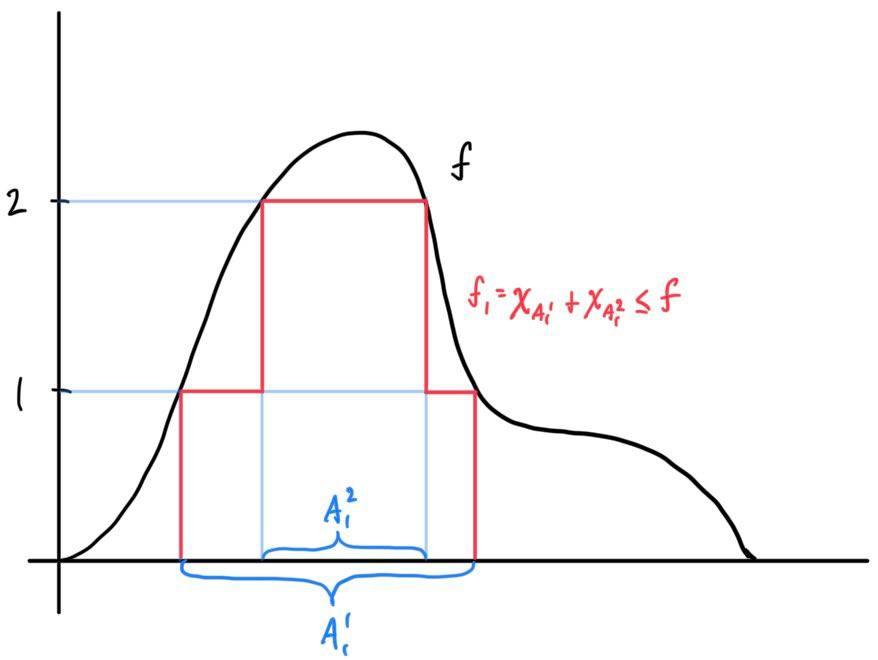
\includegraphics[scale=0.23]{img/Lebesgue_1.jpg}
\end{center}
Doing this again with finer subintervals of the codomain gives us, with $f_2 = 1_{A_2^1} + 1_{A_2^2} + 1_{A_2^3} + 1_{A_2^4} \leq f$. 
\begin{center}
    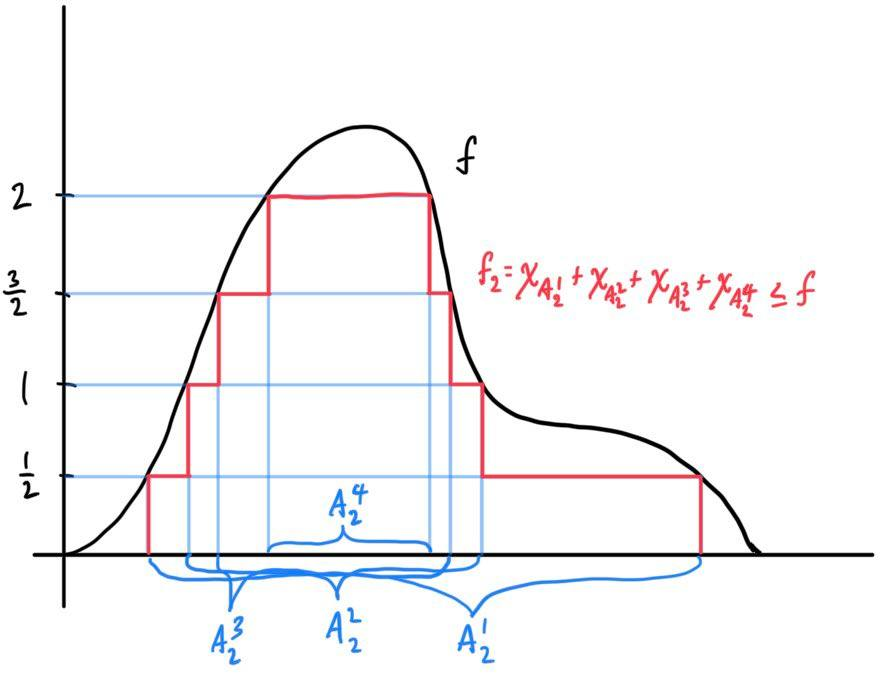
\includegraphics[scale=0.23]{img/Lebesgue_2.jpg}
\end{center}
and in general, we have $f_k = \sum_{j=1}^\infty \frac{1}{2^{k-1}} 1_{A^j_k}$. But we said a simple function is a \textit{finite} sum, and if $\infty$ is in the range of $f$, then this becomes a problem. We can quickly fix this by just truncating the summation at a certain point in the codomain ($f_1$ only considers intervals up to $1$, $f_2$ up to $2$ and so on), ultimately giving us 
\[f_k = \sum_{j=1}^{k 2^{k-1}} \frac{1}{2^{k-1}} 1_{A^j_k} \]
\end{proof}

\subsubsection{Lebesgue Integral}

Finally, we can learn how to integrate. We require the positiveness condition on $f$ below because our previous theorem on approximating arbitrary functions with simple measurable functions $f_k$ requires that it be positive, too. 

\begin{definition}[Lebesgue Integral of Positive Simple Functions]
If $f = \sum_{k=1}^n c_k 1_{A_k}$ is a positive simple Lebesgue measurable function on measure space $(X, \mathcal{A}, \mu)$, then the \textbf{Lebesgue integral} of $f$ is 
\[\int f \, d\mu = \sum_{k=1}^n c_k \mu(A_k)\]
\end{definition}

This Lebesgue integral agrees with the Riemann integral for step functions. Let $c_1, \ldots, c_n \in [0, \infty)$ and $a = x_0 < x_1 < \ldots < x_n = b$ be a partition. Let $f: [a, b] \longrightarrow [0, \infty]$ be a step function taking the value $c_i$ on the interval $(x_{i-1}, x_i)$ for $i = 1, \ldots, n$. Then the Riemann integral of $f$ is simply 
\[\int f(x) \,dx = \sum_{i=1}^n c_k |x_i - x_{i-1}|\]
The Lebesgue integral is 
\begin{align*}
    \int f \, d \mu & = \sum_{i=1}^n c_i \mu((x_{i-1}, x_i)) + \sum_{j=0}^n f(x_j) \mu(\{x_j\}) \\
    & = \sum_{i=1}^n c_k |x_i - x_{i-1}|
\end{align*}
which agrees with the Riemann integral. In the Riemann integral, we write $dx$ to indicate the variable that is being integrated over, but in the Lebesgue integral, we write $d \mu$, the measure which we are integrating over. Therefore, there are many possible values that can come out of a Lebesgue integral of a certain function, while a Riemann integral outputs only one value if exists. 

\begin{example}
Consider the simple function (consisting of one characteristic function) $1_{\mathbb{Q} \cap [0, 1]}$. $\mathbb{Q} \cap [0, 1]$ is a Lebesgue measurable set of $\mathbb{R}$, and we have $1_{\mathbb{Q} \cap [0, 1]} \geq 0$, so its Lebesgue integral is given by the above definition: 
\[\int_{\mathbb{R}} 1_{\mathbb{Q} \cap [0, 1]} \, d\lambda = 1 \cdot \lambda(\mathbb{Q} \cap [0, 1]) = 0\]
\end{example}

\begin{definition}[Lebesgue Integral on Positive Measurable Functions]
If $f: (X, \mathcal{A}, \mu) \longrightarrow [0, \infty]$ is measurable, then 
\[\int_X f \, d\mu = \sup \Big\{ \int g\, d\mu \,\Big|\, g \text{ simple }, g \leq f\Big\}\]
\end{definition}

Unlike Riemann integration, which looks at both the supremum and infimum of integrals of simple functions, Lebesgue integration only looks at the supremum, given that $f$ is nonnegative, so for all these $f$, the Lebesgue integral always exists. Defining Lebesgue integration for all real-valued functions, requires a simple extension. 

\begin{definition}[Lebesgue Integral]
Given a function $f: (X, \mathcal{A}, \mu) \longrightarrow \mathbb{R}$, we can split $f$ into a positive and negative part: 
\[f = f^+ - f^-\]
where $f^+ = \max(f, 0)$ and $f^- = \max(-f, 0)$. Then, the Lebesgue integral of $f$ is 
\[\int f \, d \mu = \int f^+ \, d\mu - \int f^- \, d\mu\]
given that at least one of these integrals is finite. If one is infinite and the other is finite, then we can call it infinite. If we have \textit{both} infinite integrals, then the integral doesn't exist. It has the properties: 
\begin{enumerate}
    \item Monotonicity: 
    \[g \leq f \implies \int g \, d\mu \leq \int f\, d\mu\]
    \item Scalar Multiplication: 
    \[\int c f \, d\mu = c \int f \, d\mu\]
    \item Addition:
    \[\int f + g \, d\mu = \int f \,d\mu + \int g \,d\mu\]
\end{enumerate}
\end{definition}

Since $|f| = f^+ + f^-$, $f$ is also Lebesgue integrable if 
\[\int |f| \, d\mu < \infty \]
since by triangle inequality, we have 
\[\bigg| \int f \, d\mu \bigg| \leq \int |f| \, d \mu\]

\begin{definition}
The set of all functions $f: (X, \mathcal{A}, \mu) \longrightarrow \mathbb{R}$ that are Lebesgue integrable is denoted $\mathcal{L}^1(X, \mathcal{A}, \mu; \mathbb{R})$, or for short $\mathcal{L}^1(X, \mathcal{A}, \mu)$. 
\end{definition}

\begin{theorem}
$f: \mathbb{R} \longrightarrow \mathbb{R}$ is Riemann integrable iff it is continuous $\lambda$ almost everywhere. If so, then $f$ is Lebesgue measurable and 
\[\int_{[a, b]} f \,d\lambda = \int_a^b f \, dx\]
for all $a < b$. 
\end{theorem}

\subsubsection{Integral Inequalities}

We introduce 3 important inequalities on the integral. 

\begin{theorem}[Jensen's Inequality]
Suppose $\phi$ is convex, that is, 
\[\lambda \phi(x) + (1 - \lambda) \phi(y) \geq \phi (\lambda x + (1 - \lambda) y)\]
for all $\lambda \in (0, 1)$ and $x, y \in \mathbb{R}$. If $\mu$ is a probability measure, and $f$ and $\varphi(f)$ are integrable, then 
\[\varphi\bigg( \int f \,d\mu \bigg) \leq \int \varphi(f) \,d\mu\]
\end{theorem}

\begin{theorem}[Holder's Inequality]
If $p, q$ are Holder conjugates, then 
\[\int |f g|\, d\mu \leq ||f||_p ||g||_q\]
\end{theorem}

\begin{corollary}[Cauchy-Schwarz Inequality]
Given that $p = q = 2$ above, then we have 
\[\int |f g|\, d\mu \leq ||f||_2 ||g||_2\]
which is similar to the familiar equation $\langle u, v \rangle \leq ||u|| ||v||$. 
\end{corollary}

\subsubsection{Convergence Theorems}

Now, we want to give conditions that guarantee 
\[\lim_{n \rightarrow \infty} \int f_n \,d \mu = \int \big( \lim_{n \rightarrow \infty} f_n \big) \, d\mu\]

\begin{definition}
A sequence of functions $f_n \rightarrow f$ \textbf{in measure} if for any $\epsilon > 0$, 
\[\mu\big( \{x \,:\, |f_n (x) - f(x)| > \epsilon \}\big) \rightarrow 0 \text{ as } n \rightarrow \infty\]
\end{definition}

\begin{theorem}[Bounded Convergence Theorem]
Let $E$ be a set with $\mu(E) < \infty$. Suppose $f_n = 0$ on $E^c$, $|f_n (x)| \leq M$, and $f_n \rightarrow f$ in measure. Then, 
\[\int f \,d\mu = \lim_{n \rightarrow \infty} \int f_n d\mu\]
\end{theorem}

\begin{lemma}[Fatou's Lemma]
If $f_n \geq 0$, then
\[\lim_{n \rightarrow \infty} \inf \int f_n \,d\mu \geq \int \Big( \lim_{n \rightarrow \infty} \inf f_n \Big) \,d\mu\]
\end{lemma}

\begin{theorem}[Monotone Convergence Theorem]
Given a nondecreasing sequence of measurable nonnegative functions $\{f_n\}$, its limit $f_n \uparrow f$ always exists (since $f_n$ is nondecreasing), is measurable, and 
\[\int f_n \, d\mu \uparrow \int f \, d\mu\]
This allows us to integrate the limit of nice functions $f_n$ by integrating these $f_n$ first and then finding what the values converge to. 
\end{theorem}

\begin{theorem}[Dominated Convergence Theorem]
If $f_n \rightarrow f$ a.e., $|f_n| \geq g$ for all $n$, and $g$ is integrable, then 
\[\int f_n \,d\mu \rightarrow \int f\, d\mu\]
\end{theorem}

\subsubsection{Product Measures, Fubini's Theorem}

Let $(X, \mathcal{A}, \mu_1)$ and $(Y, \mathcal{B}, \mu_2)$ be two measure spaces. Let 
\begin{align*}
    \Omega & = X \times Y = \{(x, y) \mid x \in X, y \in Y\} \\
    \mathcal{S} & = \{A \times B \mid A \in \mathcal{A}, B \in \mathcal{B}\}
\end{align*}
The sets in $\mathcal{S}$ are called \textbf{rectangles}. It is easy to see that $\mathcal{S}$ is a semi-algebra: 
\begin{align*}
    (A \times B) \cap (C \times D) & = (A \cap C) \times (B \cap D) \\
    (A \times B)^c & = (A^c \times B) \cup (A \times B^c) \cup (A^c \times B^c) 
\end{align*}

\begin{theorem}
There is a unique measure $\mu = \mu_1 \times \mu_2$ (or denoted $\mu_1 \otimes \mu_2$) on $\mathcal{F}$ with 
\[\mu(A \times B) = \mu_1 (A) \, \mu_2 (B)\]
\end{theorem}

\begin{theorem}[Fubini's Theorem]
Let $(X, \mathcal{A}, \mu_1)$ and $(Y, \mathcal{B}, \mu_2)$ be two measure spaces and $(X \times Y, \mathcal{F}, \mu = \mu_1 \times \mu_2)$ be their product space. Then, if $f \geq 0$ or $\int_{X \times Y} |f| \,d\mu < \infty$, then 
\[\int_X \int_Y f(x, y) \, \mu_2 \mu_1 = \int_{X \times Y} f \,d\mu = \int_Y \int_X f(x, y) \, \mu_1 \mu_2\]
\end{theorem}



\subsection{Random Vectors}

Now when we consider several random variables, they will all be defined on the same probability space. Given two random variables $X$ and $Y$ on $(\Omega, \mathcal{F}, \mathbb{P})$, they will each induce a probability law $\mathbb{P}_X$ and $\mathbb{P}_Y$ which completely characterizes them. Note that it is the same underlying randomness that is feeding these random variables, and so if I know some information about the value of $X$, then we know something about outcome $\omega$, which can be used to find something about the value of $Y$. To capture this, we can imagine the map $(X, Y) : \Omega \longrightarrow \mathbb{R}^2$ defined $(X, Y)(\omega) \coloneqq (X(\omega), Y(\omega))$. And just like how $X$ induces a measure $P_X$ onto $\mathbb{R}$, we can imagine $(X, Y)$ inducing a measure onto $\mathcal{B}(\mathbb{R}^2)$, which can be generated by all semi-infinite rectangles $(-\infty, x] \times (-\infty, y]$. Ideally, we would want to put a measure $\mathbb{P}_{X, Y}$ on $\mathbb{R}^2$ s.t. 
\[\mathbb{P}_{X, Y}(B) \coloneqq \mathbb{P}((X, Y)^{-1}(B))\]
where $(X, Y)^{-1}(B) = \{ \omega \in \Omega \mid (X(\omega), Y(\omega)) \in B\}$ denotes the preimage of $(X, Y)$. But is $(X, Y)^{-1}(B)$ $\mathcal{F}$-measurable? It turns out that it is. 

\begin{theorem}
Let $f: (X, \mathcal{A}, \mu) \longrightarrow \mathbb{R}^n$ have component functions $f_1, f_2, \ldots, f_n$. Then, $f$ is measurable (i.e. $f^{-1} (B) \in \mathcal{A}$ for all $B \in \mathcal{B}(\mathbb{R}^n)$) if and only if all of its component functions are measurable (i.e. $f_i^{-1} (B) \in \mathcal{A}$ for all $B \in \mathcal{B}(\mathbb{R}^n)$). 
\end{theorem}

From the theorem above, I have a probability law $\mathbb{P}_{X, Y}$ on all Borel sets of $\mathbb{R}^2$, making $(\mathbb{R}^2, \mathcal{B}(\mathbb{R}^2), \mathbb{P}_{X, Y})$ a probability space. Now, since $X$ and $Y$ are both random variables dependent on the same $\omega \in \Omega$, we could expect certain "combinations" of $X$ and $Y$ to be more probable than other combinations. 

\begin{definition}[Joint Probability Law]
Given two random variables $X, Y$ on $(\Omega, \mathcal{F}, \mathbb{P})$, the \textbf{joint random variable} $(X, Y): \Omega \longrightarrow \mathbb{R}^2$ is a measurable function defined 
\[(X, Y) (\omega) \coloneqq (X(\omega), Y(\omega))\]
which induces a \textbf{joint probability law} $\mathbb{P}_{X, Y}: \mathcal{B}(\mathbb{R}^2) \longrightarrow [0, 1]$ defined 
\[\mathbb{P}_{X, Y}(B) \coloneqq \mathbb{P}((X, Y)^{-1}(B)) \; \forall B \in \mathcal{R}\]
of $X, Y$. This law captures everything there is about the interdependence of $X$ and $Y$. 
\end{definition}

Given joint probability law $\mathbb{P}_{X, Y}$, we can get the probability laws of $X$ and $Y$ separately. For example, we can take a specific Borel set of $\mathbb{R}$ representing the outcomes of $X$ and look at every single combination of it with every $Y$. But knowing $\mathbb{P}_X$ and $\mathbb{P}_Y$ is not enough to know the joint $\mathbb{P}_{X, Y}$. 

\begin{definition}[Marginal Probability Law]
Given a joint probability law $\mathbb{P}_{X, Y}$ of $X, Y$, we can get the \textbf{marginal probability law} of $X$ by feeding in Borel sets of form $B \times \mathbb{R} \in \mathcal{B}(\mathbb{R}^2)$. 
\[\mathbb{P}_X (B) = \mathbb{P}_{X, Y} (B \times \mathbb{R})\]
and the marginal probability law of $Y$ as 
\[\mathbb{P}_Y (B) = \mathbb{P}_{X, Y} (\mathbb{R} \times B)\]
\end{definition}

\begin{definition}[Joint Cumulative Distribution Function]
Since sets of the form $(-\infty, x] \times (-\infty, y]$ are Borel in $\mathbb{R}^2$, the \textbf{joint cumulative distribution function} 
\begin{align*}
    F_{X, Y} & \coloneqq \mathbb{P}_{X, Y} \big( (-\infty, x] \times (-\infty, y] \big) \\
    & = \mathbb{P} \big( \{\omega \mid X(\omega) \leq x\} \cap \{ \omega \mid Y(\omega) \leq y\} \big)
\end{align*}
is well-defined. By abuse of notation, we will write $F_{X, Y} (x, y) = \mathbb{P}(X \leq x, Y \leq y)$. The marginal CDFs are defined 
\begin{align*}
    F_X (x) & \coloneqq \mathbb{P}_{X, Y} ((-\infty, x) \times \mathbb{R}) \\
    F_Y (y) & \coloneqq \mathbb{P}_{X, Y} (\mathbb{R} \times (-\infty, y))
\end{align*}
\end{definition}

\begin{lemma}[Properties of Joint CDF]
Some common properties of the joint CDF are as follows: 
\begin{enumerate}
    \item Limits. 
    \[\lim_{(x, y) \rightarrow (+\infty, +\infty)} F_{X, Y} (x, y) = 1 \text{ and } \lim_{(x, y) \rightarrow (-\infty, -\infty)} F_{X, Y} (x, y) = 0\]
    \item Monotonicity. 
    \[x_1 \leq x_2, \; y_1 \leq y_2 \implies F_{X, Y} (x_1, y_1) \leq F_{X, Y}(x_2, y_2)\]
    \item Continuity from above. 
    \[\lim_{\epsilon \rightarrow 0^+} F_{X, Y} (x + \epsilon, y + \epsilon) = F_{X, Y} (x, y) \text{ for all } x, y \in \mathbb{R}\]
    \item Maringal CDFs. 
    \[\lim_{y \rightarrow \infty} F_{X, Y} (x, y) = F_X (x), \;\;\;\; \lim_{x \rightarrow \infty} F_{X, Y} (x, y) = F_Y (y)\]
\end{enumerate}
\end{lemma}

\subsubsection{Joint Discrete Random Variables}

\begin{definition}[Joint PMF]
Given discrete random variables $X$ and $Y$, let their countable images be denoted $E_X, E_Y \subset \mathbb{R}$. Then, $E_X \times E_Y$ is also countable, and so the joint random variable $(X, Y)$ is also discrete. This means that we can write for some Borel $B$ of $\mathbb{R}^2$, 
\[\mathbb{P}_{X, Y} (B) = \sum_{(x, y) \in (E_X \times E_Y) \cap B} \mathbb{P}_{X, Y} (\{(x, y)\})\]
and we can define the PMF as $p_{X, Y} (x, y) \coloneqq \mathbb{P}_{X, Y} (\{(x, y)\})$. By abuse of notation, we write $p_{X, Y} (x, y) = \mathbb{P} (X = x, Y = y)$ and write 
\[\mathbb{P}_{X, Y} (B) = \sum_{(x, y) \in (E_X \times E_Y) \cap B} \mathbb{P} (X = x, Y = y)\]
If you give me a joint PMF $p_{X, Y}$, by the definition above this determines the entire probability law of $\mathbb{P}_{X, Y}$. 
\end{definition} 

\begin{definition}[Conditional PMF]
Let $X, Y$ be discrete random variables on $(\Omega, \mathcal{F}, \mathbb{P})$. The \textbf{conditional PMF} of $X$ given $Y = y$ is defined 
\[p_{X \mid Y} (x \mid y) \coloneqq \frac{p_{X, Y} (x, y)}{p_Y (y)} = \frac{\mathbb{P}_{X, Y} (\{x, y\})}{\mathbb{P}_Y (\{y\})}\]
and again by abuse of notation, we can simply write 
\[\mathbb{P}(X = x \mid Y = y) \coloneqq \frac{\mathbb{P}(X = x, Y = y)}{\mathbb{P}(Y = y)}\]
\end{definition}

\begin{theorem}[TFAE]
Let $X$ and $Y$ be discrete random variables. Then, the following are equivalent: 
\begin{enumerate}
    \item $X$ and $Y$ are independent. 
    \item For all $x, y \in \mathbb{R}$, the events $\{X = x\}$ (aka $X^{-1} (\{x\})$) and $\{Y = y\}$ (aka $Y^{-1} (\{y\})$) are independent. That is, 
    \[\mathbb{P} \big[ X^{-1}(\{x\}) \cap Y^{-1}(\{y\}) \big] = \mathbb{P}(X^{-1}(\{x\})) \, \mathbb{P}(Y^{-1}(\{y\}))\]
    \item For all $x, y \in \mathbb{R}$, $p_{X, Y} (x, y) = p_X (x) \cdot p_Y (y)$. 
    \item For all $x, y \in \mathbb{R}$ such that $p_Y (y) > 0$, we have $p_{X \mid Y}(x \mid y) = p_X (x)$. 
\end{enumerate}
\end{theorem}

\subsubsection{Joint Continuous Random Variables}

\begin{definition}
$X$ and $Y$ are jointly continuous if the joint law $\mathbb{P}_{X, Y}$ is absolutely continuous w.r.t. the Lebesgue measure on $\mathbb{R}^2$ (i.e. a Borel set of Lebesgue measure $0$ must have $P_{X, Y} = 0$ also). 
\end{definition}

However, $X$ and $Y$ continuous does not always imply that $(X, Y)$ are jointly continuous! If we have $X \sim \mathcal{N}(0, 1)$ and $Y = 2 X \sim \mathcal{N}(0, 4)$. Jointly continuous allows us to define a PDF on it. 

\begin{theorem}[Radon-Nikodym Theorem]
If $X$ and $Y$ are jointly continuous RVs, then there exists a measurable $f_{X, Y} : \mathbb{R}^2 \longrightarrow [0, \infty)$ s.t. for any $B \in \mathcal{B}(\mathbb{R}^2)$, we have 
\[\mathbb{P}_{X, Y} (B) = \int_B f_{X, Y} \, d\lambda\]
\end{theorem}

The Radon-Nikodym Theorem guarantees the existence of such $f_{X, Y}$. Taking $B = (-\infty, x] \times (-\infty, y]$, we can define the joint CDF as 
\[F_{X, Y} (x, y) = \mathbb{P}(X \leq x, Y \leq y) \coloneqq \mathbb{P}_{X, Y} \big( (-\infty, x] \times (-\infty, y] \bigg) = \int_{-\infty}^x \int_{-\infty}^y f_{X, Y} (s, t) \, dt \,ds\]


\subsection{Expectation}

\begin{definition}[Expectation]
Given a probability space $(\Omega, \mathcal{F}, \mathbb{P})$ and a random variable $X: \Omega \longrightarrow \mathbb{R}$, the \textbf{expectation} of $X$ is defined 
\[\mathbb{E}[X] \coloneqq \int_\Omega X \, d\mathbb{P}\]
Generally, if we are integrating over the entire probability space, then it is conventional to not write $\Omega$ in the integral at all: $\mathbb{E}[X] = \int X \,d\mathbb{P}$. 
\end{definition}

\begin{definition}[Expectation of Discrete RV]
If $X$ is a discrete random variable \textit{that takes positive values}, then let $E = \{e_1, e_2, \ldots\}$ denote the set where $\mathbb{P}_X(E) = 1$, and let $E_i = X^{-1} (\{e_i\}) \subset \Omega$. Then, we can see that since $X$ is constantly $e_i$ on $E_i$, 
\[\int_{E_i} X \, d\mathbb{P} = e_i \cdot \mathbb{P}(E_i) = e_i \cdot \mathbb{P}_X (\{e_i\}) = e_i \cdot \mathbb{P}(X = e_i)\]
which implies 
\[\mathbb{E}[X] = \int_\Omega X \, d\mathbb{P} = \sum_{i=1}^\infty \int_{E_i} X \, d\mathbb{P} = \sum_{i=1}^\infty e_i \cdot \mathbb{P}(X = e_i) \] 
If $X$ is discrete RV possibly taking negative values, then let $X = X^+ - X^-$, where $X^+ = \max(X, 0)$ and $X^- = - \min(X, 0)$. Then, we can compute 
\[\mathbb{E}[X] = \mathbb{E}[X^+] - \mathbb{E}[X^-]\]
which is well-defined as long as we don't have "$\infty - \infty$."
\end{definition}

Note that the reason why expectations of the form $\infty - \infty$ are indeterminate is because of the Riemann rearrangement theorem. 

\begin{theorem}[Riemann's Rearragenement Theorem]
Given a series $\sum a_n$ that is conditionally convergent (i.e. converges but not absolutely convergent), the terms can be arranged so that the new series converges to an arbitrary real number, or diverges. 
\end{theorem}

\begin{lemma}[Properties of Expectation]
Let $X$ and $Y$ be random variables with finite expectations. 
\begin{enumerate}
    \item Monotonicity: If $X \leq Y$ (i.e. $X(\omega) \leq Y(\omega)$ for all $\omega \in \Omega$), then 
    \[\mathbb{E}[X] \geq \mathbb{E}[Y]\]
    
    \item Non-Negativity: This is implied from the above if we set the lower bound to the constant random variable $0$. If $X \geq 0$, then 
    \[\mathbb{E}[X] \geq 0\]
    
    \item Linearity: For all $a, b, c \in \mathbb{R}$, 
    \[\mathbb{E}[a X + b Y + c] = a \mathbb{E}[X] + b \mathbb{E}[Y] + c\]
\end{enumerate}
\end{lemma}

We now show a widely-used, but nontrivial, theorem. 

\begin{theorem}[Expectation of Independent Events]
Given independent RVs $X$ and $Y$, 
\[\mathbb{E}[X Y] = \mathbb{E}[X] \, \mathbb{E}[Y]\]
\end{theorem}
\begin{proof}
We show only for simple random variables which will give us a start in proving for all random variables in full generality. Let $X$ and $Y$ be simple random variables, i.e. 
\[X = \sum_i a_i 1_{A_i} \text{ and } Y = \sum_j b_j 1_{B_j}\]
Since $\{A_i\}_i$ and $\{B_j\}_j$ are both partitions, $\{A_i \cap B_j\}_{i, j}$ is also a partition, and 
\[X Y = \sum_{i, j} a_i b_j \, 1_{A_i \cap B_j}\]
Its expectation can be expanded out by linearity, and since $\mathbb{E}[ 1_{A} ] = \mathbb{P}(A)$, we have
\begin{align*}
    \mathbb{E}[X Y] & = \sum_{i, j} a_i b_j \, \mathbb{P}(A_i \cap B_j) \\
    & = \sum_{i, j} a_i b_j \, \mathbb{P}(A_i)\, \mathbb{P}(B_j) = \mathbb{E}[X] \, \mathbb{E}[Y]
\end{align*}
Now that we have proved for simple random variables, we can just approximate $X$ from below using simple functions. 
\end{proof}

\begin{theorem}[Tail Sum Formula]
If a discrete random variable $X$ takes values in the non-negative integers $\{0, 1, 2, 3, ...\}$, then 
\[\mathbb{E}[X] = \sum_{k=1}^\infty \mathbb{P}(X \geq k)\]
In any case (continuous or discrete), if $X$ is a non-negative random variable, then 
\[\mathbb{E}[X] = \int_0^\infty \mathbb{P}(X > x) \, dx = \int_0^\infty 1 - F(x) \, dx\]
where $F$ is the CDF of $X$. 
\end{theorem}
\begin{proof}
Suppose that $X$ takes values in $\{0, 1, 2, 3, ...\}$. Then, 
\begin{align*}
    \mathbb{E}[X] & = \sum_{k \geq 1} k \, \mathbb{P}(X=k) \\
    & = \sum_{k\geq 1} \sum_{j=1}^k \mathbb{P}(X = k) \\
    & = \sum_{k \geq 1} \sum_{j=1}^k 1_{j \leq k} \, \mathbb{P}(X=k) \\
    & = \sum_{j=1}^\infty \sum_{k \geq 1} 1_{j \leq k} \, \mathbb{P}(X =k) \\
    & = \sum_{j=1}^\infty \sum_{k \geq j} \mathbb{P}(X=k) \\
    & = \sum_{j=1}^\infty \mathbb{P}(X \geq j)
\end{align*}
\end{proof}

\begin{corollary}
For any $m > 0$ and $\alpha > 0$,  
\[\mathbb{P} \big(|X| > \alpha \big) \leq \frac{1}{\alpha^m} \mathbb{E} \big( |X|^m \big)\]
\end{corollary}

\begin{example}[Geometric RV]
Recall that given $X \sim \mathrm{Geometric}(p)$, we have $\mathbb{P}(X = i) = (1 - p)^{i-1} p$ for $i \geq 1$. So, 
\[\mathbb{E}[X] = \sum_{x=1}^\infty x \, \mathbb{P}(X = x) = \sum_{x=1}^\infty x \, (1 - p)^{i-1} p = \frac{p}{(1 - (1 - p))^2} = \frac{1}{p}\]
\end{example}

\begin{example}[Infinite Expectation]
Let us have discrete random variable s.t. $\mathbb{P}(X = k) = \frac{6}{\pi^2} \frac{1}{k^2}$ for $k \geq 1$. So, 
\[\mathbb{E}[X] = \sum_{k=1}^\infty k \, \mathbb{P}(X = k) = \frac{6}{\pi^2} \sum_{k=1}^\infty \frac{1}{k} = +\infty\]
\end{example}

\begin{example}[Undefined Expectation]
Let $\mathbb{P}(X = k) = \frac{3}{\pi^2} \frac{1}{k^2}$ for $k \in \mathbb{Z}\setminus \{0\}$. The expectation of this can be computed by getting the expectation of all the positive terms and the negative terms. 
\[\mathbb{E}[X] = \mathbb{E}[X^+] - \mathbb{E}[X^{-}] = \sum_{k=1}^\infty k \cdot \frac{3}{\pi^2} \frac{1}{k^2} + \sum_{k=1}^\infty (-k) \cdot \frac{3}{\pi^2} \frac{1}{k^2} = \infty - \infty\]
Note that by the Riemann rearrangement theorem, we can't just say that the expectation is $0$ since the terms "cancel out." We could only do this if the series is absolutely convergent also, which works if $X$ takes positive values only. 
\end{example}

Note that when we compute expectation, what we do it multiply the PMF/PDF by $x$ and sum/integrate over it. The Cauchy distribution is a power function of form $\frac{1}{x^2}$, so if we multiply it by $x$, we have the new $\frac{1}{x}$ which is divergent. 

\subsubsection{Law of the Unconscious Statistician}

Given probability space $(\Omega, \mathcal{F}, \mathbb{P})$ and a random vector $X: \Omega \rightarrow \mathbb{R}^n$, this induces a probability law $\mathbb{P}_X$ acting as a measure on $\mathbb{R}^n$. Assume that this probability law $\mathbb{P}_X$ is known. Now introduce a function $g: \mathbb{R}^n \rightarrow \mathbb{R}$. We can create a new random variable $Y = g \circ X : \Omega \rightarrow \mathbb{R}$ with its own probability law $\mathbb{P}_Y$ on $\mathbb{R}$. Since we already know the probability distribution of $X$, so we can easily get the expected value of $X$ as (in the discrete case) 
\[\mathbb{E}[X] = \sum_{x \in \mathcal{X}} x \cdot \mathbb{P}(X = x)\]
where $\mathcal{X}$ is the support of $X$. But what if we wanted to get the expected value of $Y$? 
\[\mathbb{E}[Y] = \sum_{y \in \mathcal{Y}} y \cdot \mathbb{P}(Y = y) = ?\]
The problem is that we don't know the probability distribution of $Y$. But since we know that all the values of $X$ are transformed by $g$, we are taught to compute it in terms of the probability distribution of $X$. 
\[\mathbb{E}[Y] = \sum_{x \in \mathcal{X}} g(x) \cdot \mathbb{P}(X = x)\]
This "identity" that is often used must actually be treated as a rigorous theorem. This is like a change of basis formula that allows us to shift to a convenient space to compute integrals. 

\begin{theorem}[LOTUS]
Given probability space $(\Omega, \mathcal{F}, \mathbb{P})$, a random variable $X: \Omega \rightarrow \mathbb{R}^n$, and a function $g: \mathbb{R}^n \rightarrow \mathbb{R}$, the expectation of $g(X)$ is 
\[\mathbb{E}[g(X)] = \int_\Omega g(X) \,d\mathbb{P} = \int_{\mathbb{R}^n} g \, d\mathbb{P}_X = \int_\mathbb{R} \,d \mathbb{P}_{g(X)}\]
It is usually the case that we don't know the distribution of $g(X)$ since $g$ is too complicated (hard to compute the right integral) and we don't want to integrate over an abstract space $\Omega$ where we can't do calculus on (hard to compute the left integral). But we do know the distribution of $X$, so we can indeed compute the middle integral. 
\end{theorem}

Note that if $g: \mathbb{R} \rightarrow \mathbb{R}$ is the identity function $\mathrm{id}$, then we have 
\[\mathbb{E}[X] = \int_\Omega X \,d\mathbb{P} = \int_{\mathbb{R}} \mathrm{id} \, d\mathbb{P}_X\]
\begin{enumerate}
    \item For the discrete case, the above integral simplifies to 
    \[\mathbb{E}[g(X)] = \int_{\mathbb{R}^n} g \,d \mathbb{P}_X = \sum_{x \in \mathcal{X} \subset \mathbb{R}^n} g(x) p_X (x)\]
    
    \item For the continuous case, we have 
    \[\mathbb{E}[g(X)] = \int_{\mathbb{R}^n} g \,d \mathbb{P}_X = \int_{\mathbb{R}^n} g (x) \, f_X (x) \,dx \]
\end{enumerate}

\subsubsection{Expectation w.r.t. Different Measures}
Sometimes, we just write the expectation of a measurable function $f: (S, \mathcal{S}) \rightarrow \mathbb{R}$ as $\mathbb{E}[f]$. If we need to specify with respect to what measure we are integrating over, we write 
\[\mathbb{E}_\mu [f] \coloneqq \int_S f \, d\mu\]
Usually, if $f$ represents some transformation of a random variable $X: \Omega \rightarrow S$, then we assume that we are integrating w.r.t. the probability measure $\mathbb{P}$ defined on $\Omega$ or the probability law $\mathbb{P}_X$ induced by $X$. 
\[\mathbb{E}[f] = \mathbb{E}[f(X)] = \int_\Omega f(X) \,d\mathbb{P} = \int_S f \,d\mathbb{P}_X\]

\begin{example}[Expectation of Exponential RV]
The PDF of exponential random variable $X$ is defined $f_X = k e^{-k x}$ for $x \geq 0$. So, 
\[\mathbb{E}[X] = \int_\mathbb{R} x f_X \, d\lambda = \int_0^\infty x k e^{-k x} \, dx = \frac{1}{k}\]
Similarly, if we want the expectation of $X^2$, then we can get 
\[\mathbb{E}[X^2] = \int_\mathbb{R} x^2 f_X \,d\lambda = \int_0^\infty x^2 k e^{-k x} \,dx = \frac{2}{k^2}\]
\end{example} 

\begin{example}[Expectation of Gaussian RV]
The expectation of a Gaussian random variable $X$ is
\[\mathbb{E}[X] = \int_{-\infty}^\infty x \cdot \frac{1}{\sigma \sqrt{2\pi}} e^{-\frac{(x - \mu)^2}{2 \sigma^2}} \, dx = \mu\]
\end{example}

\begin{example}[Expectation of One-Sided Cauchy]
If we have $f_X (x) = \frac{2}{\pi} \frac{1}{1 + x^2}$ for $x \geq 0$, then 
\[\mathbb{E}[X] = \int_0^\infty \frac{2}{\pi} \frac{x}{1 + x^2} \,dx\]
and making the substitution $t = \frac{1 + x^2}, \; dt = 2x$, we have 
\[\int_1^\infty \frac{1}{\pi} \frac{1}{t} \,dt = \frac{\ln(t)}{\pi} \bigg|_1^\infty = +\infty\]
\end{example}

\begin{example}[Expectation of Two-Sided Cauchy]
The two-sided Cauchy is just another copy of the one sided into the negatives, so $f_X (x) = \frac{1}{\pi} \frac{1}{1 + x^2}$ for $x \in \mathbb{R}$. The expectation of $X$ should be split up into for positive and negative images, but computing it gives 
\[\mathbb{E}[X] = \mathbb{E}[X^+] - \mathbb{E}[X^-] = \int_0^\infty \frac{1}{\pi} \frac{x}{1 + x^2}\,dx - \int_{-\infty}^0 \frac{1}{\pi} \frac{x}{1 + x^2}\,dx = \infty - \infty\]
and so it is undefined. 
\end{example}

With LOTUS, we can make sense of an extremely important inequality. 

\begin{theorem}[Jensen's Inequality]
If $f$ is a convex function, then $\mathbb{E}[f(X)] \geq f (\mathbb{E}[X])$. 
\end{theorem}
\begin{proof}
We will assume that $f$ is differentiable for simplicity and let $\mathbb{E}[X] = \mu$. Define the linear function centered at $\mu$ to be $l(x) \coloneqq f(\mu) + f^\prime (\mu) (x - \mu)$. Then, we know that $f(x) \geq l(x)$ for all $x$, so 
\begin{align*}
    \mathbb{E}[f(X)] & \geq \mathbb{E}[ l(X)] \\ 
    & = \mathbb{E}[f(\mu) + f^\prime (\mu) \, (X - \mu)] \\
    & = \mathbb{E}[f(\mu)] + f^\prime (\mu) ( \mathbb{E}[X] - \mu) \\
    & = \mathbb{E}[f(\mu)] \\
    & = f(\mathbb{E}[X])
\end{align*}
\end{proof}

\subsection{Variance, Covariance, Correlation}

\begin{definition}[Variance]
Let $X$ be a random variable and suppose $\mathbb{E}[X] < \infty$. The \textbf{variance} of $X$ is defined 
\[\mathrm{Var}[X] = \sigma^2_X \coloneqq \mathbb{E} [ (X - \mathbb{E}[X])^2 ]\]
and $\sigma_X = \sqrt{\mathrm{Var}[X]}$ is called the \textbf{standard deviation}. This is a measure of how much the probability distribution deviates from its mean. We can use linearity of expectation to write 
\begin{align*}
    \mathrm{Var}[X] & = \mathbb{E} \big[ X^2 + \mathbb{E}[X]^2 - 2 X \mathbb{E}[X] \big] \\
    & = \mathbb{E}[X^2] + \mathbb{E}[X]^2 - 2 \mathbb{E}[X] \mathbb{E}[X] \\
    & = \mathbb{E}[X^2] - \mathbb{E}[X]^2
\end{align*}
which is often easier to compute, since it only requires us to compute the expectation of $X$ and $X^2$. Since variance is always nonnegative, we also know that $\mathbb{E}[X^2] \geq \mathbb{E}[X]^2$. The variance is always defined, whether it's finite or $+\infty$. 
\end{definition}

Likewise for expectation, the variance of a function $f$ w.r.t. $\mu$ is 
\[\Var_\mu (f) = \mathbb{E}_\mu [f^2] - \mathbb{E}_\mu [f]^2\]

\begin{proposition}
The variance of a random variable $X$ is $0$ if and only if it constant almost everywhere on $\Omega$. 
\end{proposition}
\begin{proof}
The if part is easy, so let's prove the only if part. Let $\mathbb{E} [ (X - \mathbb{E}[X])^2 ] = 0$. Then, we can think of the function $x \mapsto (x - \mathbb{E}[X])^2$ and write the variance as 
\[\mathrm{Var}[X] = \int_\Omega (X - \mathbb{E}[X])^2 \, d\mathbb{P} = 0\]
But by nonnegativity of the function, we know that $(X - \mathbb{E}[X])^2 = 0$ w/ probability $1$, which implies that $X = \mathbb{E}[X]$ with prob. $1$. 
\end{proof}

\begin{lemma}[Properties of Variance]
Let $X$ and $Y$ be random variables with well-defined variances. 
\begin{enumerate}
    \item Translation Invariance: Given that $X + a$ is a new random variable defined $(X + a)(\omega) = X(\omega) + a$, 
    \[\mathrm{Var}[X] = \mathrm{Var}[X + a]\]
    \item Quadratic Scaling: Given that $aX$ is a new random variable defined $(aX)(\omega) = a\,X(\omega)$, 
    \[\mathrm{Var}[aX] = a^2 \mathrm{Var}[X]\]
\end{enumerate}
\end{lemma}

From the properties of expectation and variance, we can now \textbf{standardize} a random variable $X$. If $X$ is a random variable with mean $\mu = \mathbb{E}[X]$ and variance $\sigma^2 = \Var(X)$, then the random variable 
\[Y = \frac{X - \mu}{\sigma}\]
has mean $\mathbb{E}(Y) = 0$ and variance $\Var(Y) = 1$. 

\begin{example}[Bernoulli]
Given $X \sim \mathrm{Bernoulli}(p)$, we have
\begin{align*}
    \mathbb{E}[X] & = 0 \cdot \mathbb{P}(X = 0) + 1 \cdot \mathbb{P}(X = 1) = p \\
    \mathbb{E}[X^2] & =  0^2 \cdot \mathbb{P}(X = 0) + 1^2 \cdot \mathbb{P}(X = 1) = p
\end{align*}
and so $\mathrm{Var}[X] = p - p^2 = p(1 - p)$. 
\end{example}

\begin{example}[Poisson]
Given $X \sim \mathrm{Poisson}(X)$, then 
\begin{align*}
    \mathbb{E}[X] & = \sum_{k = 0}^\infty k \cdot \frac{e^{-\lambda} \lambda^k}{k!} = \sum_{k = 1}^\infty \cdot \frac{e^{-\lambda} \lambda^k}{(k-1)!} = \lambda \sum_{k = 1}^\infty \cdot \frac{e^{-\lambda} \lambda^{k-1}}{(k-1)!} = \lambda\\
    \mathbb{E}[X] & = \sum_{k=0}^\infty k^2 \cdot \frac{e^{-\lambda} \lambda^k}{k!} = \ldots = \lambda^2 + \lambda
\end{align*}
So $\mathrm{Var}[X] = \lambda^2 + \lambda - \lambda^2 = \lambda$. 
\end{example}

\begin{example}[Uniform]
Let $X \sim \mathrm{Uniform}[a, b]$. Then, 
\begin{align*}
    \mathbb{E}[X] & = \int_\mathbb{R} x f_X \, d\lambda = \int_a^b x \cdot \frac{1}{b - a}\,dx = \frac{a + b}{2} \\
    \mathbb{E}[X^2] & = \int_\mathbb{R} x^2 f_X \,d\lambda = \int_a^b \frac{x^2}{b - a} \,dx = \frac{a^2 + ab + b^2}{3} 
\end{align*}
So $\mathrm{Var}[X] = \ldots = \frac{1}{12} (b - a)^2$. This is consistent with the fact that if we spread out our measure over a wider interval, then the variance will be bigger. 
\end{example}

\begin{example}[Exponential]
Let $X \sim \mathrm{Exp}(\lambda)$. Then, $\mathbb{E}[X] = \frac{1}{\lambda}$ and $\mathbb{E}[X^2] = \frac{2}{\lambda^2}$, so 
\[\mathrm{Var}[X] = \frac{1}{\lambda^2}\]
This is consistent with the fact that if $\lambda$ is greater, then the PDF is much more concentrated at $0$, making the variance small. 
\end{example}

Just like how we explained that computing finiteness or infiniteness of expectation is similar to multiplying the PMF/PDF by $x$ and determining if the series/integral converges or diverges, we can do the same for variance by multiplying the PMF/PDF by $x^2$. For a probability distribution of form $\frac{1}{x^2}$, it diverges if we multiply by $x$ and also diverges if we multiply by $x^2$. But also, we could construct a distribution where the expectation may be finite, but the variance may be infinite. For example, if we have a distribution of form $\frac{1}{x^3}$, multiplying it by $x$ leads to form $\frac{1}{x^2}$, which is finite (so finite expectation), but multiplying by $x^2$ leads to a harmonic, i.e. infinite variance. 

\begin{definition}[Moment]
The \textbf{$\mathbf{n}$th (raw) moment} of a random variable $X$ is $\mathbb{E}[X^n]$. Unlike the raw moment, which is calculated around the origin, the \textbf{$\mathbf{n}$th central moment} of $X$ is its moment centered around its mean $\mathbb{E}[(X - \mathbb{E}[X])^n]$. 
\begin{enumerate}
    \item the first moment is the mean $\mathbb{E}[X]$
    \item the second central moment is the variance $\mathbb{E}[(X - \mathbb{E}[X])^2]$ 
    \item the third central moment, divided by $\sigma^3$, is the skew $\frac{1}{\sigma^3} \mathbb{E}[(X - \mathbb{E}[X])^3]$ 
\end{enumerate}
\end{definition}

The variance is a measure for one random variable $X$, which measures how much it deviates from its mean. Now, the covariance is defined for two random variables and captures how they jointly vary. 

\begin{definition}[Covariance]
The \textbf{covariance} of random variables $X$ and $Y$ is defined as 
\begin{align*}
    \mathrm{Cov}[X, Y] & = \mathbb{E} \big[ (X - \mathbb{E}[X]) (Y - \mathbb{E}[X]) \big] \\
    & = \mathbb{E}[X Y] - \mathbb{E}[X] \, \mathbb{E}[Y]
\end{align*}
where the intermediate expectations are well-defined. $X$ and $Y$ are said to be \textbf{uncorrelated} if 
\[\mathrm{Cov}[X, Y] = 0\]
\end{definition}

The covariance is also easy to interpret. Given two random variables $X$ and $Y$, if whenever $X$ is greater than its expected value $\mathbb{E}[X]$, $Y$ also tends to be greater than $\mathbb{E}[Y]$, then the covariance will be some positive number. If they tend to be on opposite sides of their expected values, then the covariance will be negative. And the degree with which these RVs lie on which side of the expected value determines the magnitude of the covariance. 

\begin{theorem}
If $X$ and $Y$ are independent random variables, then they are uncorrelated, meaning that independence is a stronger condition. 
\end{theorem}

We show an example of why the converse is not true. Consider $X \sim \mathrm{Uniform}[-1, 1]$. We can show that $x$ and $Y = X^2$ are dependent but uncorrelated. It is clearly dependent, but its covariance is 
\begin{align*}
    \mathrm{Cov}(X, Y) & = \mathbb{E}[X Y] - \mathbb{E}[X] \, \mathbb{E}[Y] \\
    & = \mathbb{E}[X^3] - \mathbb{E}[X] \, \mathbb{E}[X^2] \\
    & = \int_{-1}^1 x^3 \cdot 1 \,dx - 0 \cdot \mathbb{E}[X^2] = 0
\end{align*}

\begin{theorem}
If $X$ and $Y$ are two random variables, then 
\[\mathrm{Var}(X + Y) = \mathrm{Var}[X] + \mathrm{Var}(Y) + 2 \mathrm{Cov}(X, Y)\]
and by induction, we can show that 
\[\mathrm{Var}\bigg( \sum_i X_i\bigg) = \sum_{i} \mathrm{Var}(X_i) + \sum_{i, j} \mathrm{Cov}(X_i, X_j) \]
\end{theorem}
\begin{proof}
Simple computation. The LHS expands to 
\begin{align*}
    \mathbb{E}[(X + Y)^2] - \mathbb{E}[X + Y]^2 & = \mathbb{E}[X^2 + 2XY + Y^2] - (\mathbb{E}[X] + \mathbb{E}[Y])^2 \\
    & = \mathbb{E}[X^2] + 2 \mathbb{E}[XY] + \mathbb{E}[Y^2] - \mathbb{E}[X]^2 - 2 \mathbb{E}[X] \mathbb{E}[Y] - \mathbb{E}[Y]^2 \\
    & = \big( \mathbb{E}[X^2] - \mathbb{E}[X]^2 \big) + \big( \mathbb{E}[Y^2] - \mathbb{E}[Y]^2 \big) + 2 \big( \mathbb{E}[XY] - \mathbb{E}[X] \mathbb{E}[Y] \big) \\
    & = \mathrm{Var}[X] + \mathrm{Var}(Y) + 2 \mathrm{Cov}(X, Y) 
\end{align*}
\end{proof}

Therefore, if we have $n$ random variables $X_1, \ldots, X_n$, then we can compute their pairwise covariance $\mathrm{Cov}(X_i, X_j)$ and compute their \textbf{covariance matrix} $\boldsymbol{\Sigma}$, which is an $n \times n$ symmetric matrix with entries 
\[\boldsymbol{\Sigma}_{ij} = \mathrm{Cov}(X_i, X_j) \text{ for } i, j = 1, \ldots, n\]

Finally we define the correlation. 

\begin{definition}[Correlation Coefficient]
The \textbf{correlation coefficient} of random variables $X$ and $Y$ is defined 
\[\rho_{X, Y} = \mathrm{Corr}(X, Y) \coloneqq \frac{\mathrm{Cov}(X, Y)}{\sigma_X \sigma_Y} = \frac{\mathrm{Cov}(X, Y)}{\sqrt{\mathrm{Var}[X] \, \mathrm{Var}(Y)}}\]
\end{definition}

\subsubsection{Hilbert Space of Random Variables}

In some sense the correlation is a scaled version of the covariance. It is scale-invariant, and it is always a number that lies between $-1$ and $1$, making it a nice way to represent the correlation between two variables without having to worry about scale. We can prove this. 

\begin{theorem}[Cauchy-Schwartz]
For any two random variables $X, Y$, we have $|\mathrm{Cov}(X, Y)| \leq \sigma_X \sigma_Y$, or in other words, 
\[-1 \leq \rho_{X, Y} \leq 1\]
Furthermore, whenever $\rho_{X, Y} = 1$ or $-1$, there exists a deterministic relationship between $X$ and $Y$. 
\begin{enumerate}
    \item If $\rho_{X, Y} = 1$, there exists a $a > 0$ s.t. 
    \[Y - \mathbb{E}[Y] = a (X - \mathbb{E}[X])\]
    \item If $\rho_{X, Y} = -1$ there exists a $a < 0$ s.t. 
    \[Y - \mathbb{E}[Y] = a (X - \mathbb{E}[X])\]
\end{enumerate}
This implies that $\Corr(X, Y) = \pm 1$ indicates that the joint distribution of $(X, Y)$ is concentrated on a line in $\mathbb{R}^2$. 
\end{theorem}

The fact that this is called the Cauchy-Schwartz inequality hints at the existence of inner products, norms, and vector spaces. That is, we can treat the random variables $X, Y$ as vectors in the functional space of real-valued maps over $\Omega$. In some sense, $\mathrm{Cov}(X, Y)$ sort-of plays the role of an inner product. 
\begin{enumerate}
    \item It satisfies symmetricity: 
    \[\mathrm{Cov}(X, Y) = \mathbb{E}[X Y] - \mathbb{E}[X] \, \mathbb{E}[Y] =  \mathbb{E}[Y X] - \mathbb{E}[Y] \, \mathbb{E}[X] = \mathrm{Cov}(Y, X)\] 
    
    \item It satisfies binlinearity. It suffices to show only for first argument, since we have symmetricity. 
    \begin{align*}
        \mathrm{Cov}(aX + bY, Z) & = \mathbb{E}[(a X + b Y) Z] - \mathbb{E}[a X + b Y] \, \mathbb{E}[Z] \\
        & = a \mathbb{E}[X Z] + b \mathbb{E}[Y Z] - a \mathbb{E}[X] \mathbb{E}[Z] - b \mathbb{E}[Y] \, \mathbb{E}[Z] \\
        & = a \big( \mathbb{E}[X Z] - \mathbb{E}[X] \mathbb{E}[Z] \big) + a \big( \mathbb{E}[Y Z] - \mathbb{E}[Y] \, \mathbb{E}[Z] \big) \\
        & = a \, \mathrm{Cov}(X, Z) + b \, \mathrm{Cov}(Y, Z)
    \end{align*}

    \item We want the inner product of $X$ with itself to always be greater than $0$, with equality holding iff $X = 0$. Indeed, we have 
    \[\mathrm{Cov}(X, X) = \mathrm{Var}[X] \geq 0\]
    but it is not necessarily true that $\mathrm{Var}[X] = 0 \implies X = 0$. We can say that $X$ is equal to a constant almost everywhere at best. We can solve this problem by looking at the functional subspace of $0$-mean random variables (which is a vector space due to linearity of expectation). So now all random variables $X$ that are $0$ almost everywhere have inner product $0$, so we must add an equivalence class on this subspace that says two $X, Y$ are equivalent if they agree almost everywhere. 
\end{enumerate}
The standard deviation $\sigma_X$ and $\sigma_Y$ act as norms on this quotient subspace of $0$-mean random variables. So the correlation coefficient $\rho_{X, Y}$ can be interpreted as the cosine of the angle between $X$ and $Y$. This now makes our desired space a Hilbert space, and our uncorrelated random variables are like orthogonal vectors. 

\begin{definition}
Let $L^2_\mathcal{F} (\Omega)$ be the function space consisting of equivalence classes of $0$-mean random variables $X: (\Omega, \mathcal{F}) \rightarrow \mathbb{R}$ that are almost surely equal. Then, 
\begin{enumerate}
    \item we can define the inner product on this space as 
    \[\langle X, Y \rangle \coloneqq \mathbb{E}[X Y] - \mathbb{E}[X] \mathbb{E}[Y] = \mathbb{E}[X Y] = \int_\Omega X Y \,d\mathbb{P}\]

    \item which induces the $L^2$-norm on this space defined 
    \[||X||_2 \coloneqq \mathrm{Var}(X) = \mathbb{E}[X^2] - \mathbb{E}[X]^2 = \mathbb{E}[X^2] = \int_\Omega X^2 \,d\mathbb{P}\]
\end{enumerate}
We set $L^2_\mathcal{F} (\Omega)$ to be a Banach space with bounded norm $\mathbb{E}[X^2] < \infty$. 
\end{definition}

\section{Convergence}

\subsection{Borel-Cantelli Lemmas}

There are many Borel-Cantelli lemmas, and we will introduce the two most famous ones. To understand what these lemmas say, given a sequence $A_1, A_2, \ldots$ of events in $\sigma$-algebra $\mathcal{F}$, we must first understand what the daunting term  
\[\bigcap_{n=1}^\infty \bigcup_{i = n}^\infty A_i\]
means. Now let's try to explain what the intersection of the unions mean. First, remember that $\sigma$-algebras are stable under both countable unions and countable intersections, this is also in $\mathcal{F}$. We can interpret 
\[\bigcap_{n=1}^\infty \bigcup_{i=n}^\infty A_i = \{ A_n \text{ i.o.}\} \]
as the \textit{event that infinitely many $A_n$'s occur}, where i.o. means "infinitely often." To parse this, let's start from the innermost term and call it 
\[B_n = \bigcup_{i=n}^\infty A_i \implies \{A_n \text{ i.o.}\} = \bigcap_{n=1}^\infty B_n\]
$B_n$ is the event that at least one of the $A_n, A_{n+1}, A_{n+2}, \ldots$ occurs, often referred to as the \textit{$n$th tail event}. Now the intersection of all $B_n$'s is the event that \textit{all} $B_n$'s occur. In other words, this is the event that for no matter how big of an $N \in \mathbb{N}$ I choose, there is always at least an event $A_n$ with $n > N$ that occurs. This is shortly summarized as the event that infinitely many $A_n$'s occur. 

\begin{lemma}[1st Borel-Cantelli Lemma]
Given probability space $(\Omega, \mathcal{F}, \mathbb{P})$, if $A_1, A_2, \ldots$ is a sequence of events such that 
\[\sum_{n=1}^\infty \mathbb{P}(A_n) < \infty\]
the almost surely (with probability $1$) only finitely many $A_n$'s will occur. 
\[\mathbb{P} \bigg( \bigcap_{n=1}^\infty \bigcup_{i = n}^\infty A_i \bigg) = 0\]
\end{lemma}
\begin{proof}
Setting $B_n$ as above, we have 
\begin{align*}
    \mathbb{P}\bigg( \bigcap_{n=1}^\infty B_n \bigg) & = \lim_{n \rightarrow \infty} \mathbb{P}(B_n) & (\text{continuity of probability}) \\
    & = \lim_{n \rightarrow \infty} \mathbb{P} \bigg( \bigcup_{i=1}^\infty A_i \bigg) & (\text{substitute } B_i) \\
    & \leq \lim_{n \rightarrow \infty} \sum_{i = n}^\infty \mathbb{P}(A_i) = 0 & (\text{tail sum of convergent series is } 0)
\end{align*}
\end{proof}

The second Borel-Cantelli lemma is like a partial contrapositive to the first lemma, where it starts with the assumption that the sum of the $\mathbb{P}(A_n)$'s are infinite (along with the addition case that they are independent). 

\begin{lemma}[2nd Borel-Cantelli Lemma]
If $A_1, A_2, \ldots$ are independent events such that 
\[\sum_{n=1}^\infty \mathbb{P}(A_n) = \infty,\]
then almost surely (with probability $1$) infinitely many $A_n$'s will occur. That is, 
\[\mathbb{P} \bigg( \bigcap_{n=1}^\infty \bigcup_{i = n}^\infty A_i \bigg) = 1\]
\end{lemma}

The intuition behind this lemma is challenging: We can let $\mathbb{P}(A_n) = P_n$ and interpret the sum as a series of $P_n$'s. Since the series $P_1 + P_2 + \ldots$ is finite, this implies that 
\[\lim_{n \rightarrow \infty} P_n = 0\]
(but not the converse) and going to zero rather fast such that the series is finite. So, you are working with a sequence of events $A_n$ that are becoming more and more unlikely rather fast. The lemma says that beyond a certain point $n_0$, none of the events $A_n$ will occur almost surely. For the second lemma, we can go as far as we like in the sequence of $A_n$'s, up to any $A_{n_0}$, but beyond that there is always an infinite number of $A_n$'s that occur beyond $A_{n_0}$. 

\subsection{Transforms}

\subsubsection{Probability Generating Function (PGF)}

The PGF is only defined for discrete random variable, and is analogous to the Z-transform in singal processing. 

\begin{definition}[Probability Generating Function]
Let $X$ be a discrete random variable taking values in $\mathbb{N}_0$. Then, the \textbf{probability generating function} of $X$ is defined 
\[G_X (z) \coloneqq \mathbb{E}[z^X] = \sum_{i=0}^\infty z^i \, \mathbb{P}(X = i)\]
Now there is the problem of convergence, but we will not pay attention to this technicality for now and just consider the PGF as a tool. 
\end{definition}

\begin{example}[PGF of Poisson]
The random variable $X \sim \mathrm{Poisson}(\lambda)$ has pmf $\mathbb{P}(X = i) = \frac{e^{-\lambda} \lambda^i}{i!}$ for $i \in \{0, 1, \ldots\}$. Then, 
\[G_X (z) = \mathbb{E}[z^X] = \sum_{i=0}^\infty z^i \, \frac{e^{-\lambda} \lambda^i}{i!} = \sum_{i=0}^\infty \frac{e^{-\lambda} (\lambda z)^i}{i!} = e^{\lambda(z - 1)}\]
\end{example}

\begin{example}[PGF of Geometric]
For $X \sim \mathrm{Geometric}(p)$, its PGF is 
\[G_X (z) = \sum_{i=1}^\infty z^i \, (1 - p)^i p = \frac{p z}{1 - z(1 - p)}\]
\end{example}

\begin{lemma}[Properties of PGF]
Given random variable $X$ and its PGF $G_X$, we have the following: 
\begin{enumerate}
    \item Evaluate at $z = 1$: 
    \[G_X (1) = \mathbb{E}[1^X] = \mathbb{E}[1] = 1\]
    \item Derivative at $z = 1$: 
    \[\frac{d G_X (z)}{d z} \bigg|_{z = 1} = \mathbb{E}[X]\]
    \item $k$th derivative at $z = 1$: 
    \[\frac{d^k G_X (z)}{d z^k} \bigg|_{z = 1} = \mathbb{E}[X (X-1) (X-2) \ldots (X-k +1)]\]
    \item Transformation: Given the sum $Z = X + Y$ (where $X, Y$ are independent), rather than computing its convolution, the PGF of $Z$ is simply the product of the PGFs of $X$ and $Y$: 
    \[G_Z (z) = G_X (z) \, G_Y (z)\]
    For example, since a $\mathrm{Poisson}(\lambda)$ random variable has PGF of form $e^{\lambda (z - 1)}$, if we have two Poissons $X$ and $Y$ with parameters $\lambda, \mu$, then we can easily multiply their PGFs to get the PGF of $Z = X + Y$, which is $e^{(\lambda + \mu)(z - 1)}$, which is the PGF of a $\mathrm{Poisson}(\lambda + \mu)$ random variable. 
\end{enumerate}
\end{lemma}

\subsubsection{Moment Generating Function (MGF)}

\begin{definition}[Moment Generating Function (MGF)]
The \textbf{moment generating function} associated with a random variable $X$ is a function $M_X: \mathbb{R} \longrightarrow [0, \infty]$ defined 
\[M_X (s) \coloneqq \mathbb{E}[e^{s X}] \]
It is like an exponential moment. The region of convergence of $M_X$ is the set $D_X = \{s \mid M_X (s) < \infty\}$. 
and we always have $M_X (0) = 1$, so $0 \in D_X$ always. 
\end{definition}

\begin{lemma}[Properties of MGF]
Let $X$ be a random variable with MGF $M_X (s)$. 
\begin{enumerate}
    \item $M_X (0) = 1$, so $0$ is always in the region of convergence. 
    \item If $Y = a X + b$, then 
    \[M_Y (s) = e^{b s} M_X (a s)\]
    \item If $X$ and $Y$ are independent and $Z = X + Y$, then 
    \[M_Z (s) = M_X (s) \, M_Y (s)\]
\end{enumerate}
\end{lemma}
\begin{proof}
Listed. 
\begin{enumerate}
    \item $M_X (0) = \mathbb{E}[e^{0 X}] = \mathbb{E}[1] = 1$. 
    \item We have 
    \begin{align*}
        M_Y (s) & = \mathbb{E} [e^{s(a X + b)}] \\
        & = \mathbb{E}[ e^{a s X } e^{b s}] \\
        & = \mathbb{E}[e^{(as) X}] \, \mathbb{E}[e^{b s}] \\
        & = e^{b s} M_X (a s)
    \end{align*}
    where the penultimate step was due to independence of constant RV with any other RVs. 
    \item We can see 
    \[M_Z (s) = \mathbb{E}[ e^{s (X + Y)}] = \mathbb{E}[e^{s X} \, e^{s Y}] = \mathbb{E}[e^{s X}] \, \mathbb{E}[e^{s Y}] = M_X (s) \, M_Y (s)\]
    since $X, Y$ independent means that any function of $X$ and $Y$ are independent. 
\end{enumerate}
\end{proof}

\begin{theorem}[Inversion Theorem]
Suppose $M_X (s)$ is finite for all $s \in [-\epsilon, \epsilon]$ for some $\epsilon > 0$. Then, $M_X$ uniquely determines the CDF of $X$. This implies that if $X$ and $Y$ are random variables such that $M_X (s) = M_Y (s)$ for all $s \in [-\epsilon, \epsilon]$ for some $\epsilon > 0$, then $X$ and $Y$ have the same CDF. 
\end{theorem}

This theorem is useful for comparing random variables with the MGFs, but a limitation is that it is not always clear that the MGF is defined beyond $0$. Now, we explain why this is called a moment generating function. 

\begin{theorem}[Moment Generating Property]
Suppose $M_X (s) < \infty$ for $s \in [-\epsilon, \epsilon]$ with $\epsilon > 0$. Then, the derivatives at $s = 0$ generate the moments of $X$: 
\[\frac{d^m M_X (s)}{d s^m} \bigg|_{s = 0} = \mathbb{E}[X^m]\]
\end{theorem}
\begin{proof}
A hand-wavy proof is that we can take the derivative and put it "in" the expectation. 
\[\frac{d}{ds} \mathbb{E}[e^{s X}] = \mathbb{E} \big[ \frac{d}{ds} e^{s X} \big] = \mathbb{E}[X e^{s X}]\]
which evaluates to $\mathbb{E}[X]$ when $s = 0$. Differentiating $m$ times just gets $\mathbb{E}[X^m e^{s X}]$. However, this should be questioned, since the expectation is an integral and we are putting the derivative inside the integral. 
\end{proof}

\begin{example}[Exponential RV]
The PDF of $X \sim \mathrm{Exponential}(\mu)$ is $f_X (x) = \mu e^{-\mu x}$ for $x \geq 0$. The MGF is 
\[M_X (s) \coloneqq \int_0^\infty \mu e^{-\mu x} e^{s x} \, dx = \begin{cases} 
    \frac{\mu}{\mu - s} & \text{ for } s < \mu \\
    \infty & \text{ for } s \geq \mu 
\end{cases} \]
\end{example}

\begin{example}[Gaussian RV]
The PDF of a standard Gaussian $X$ is $f_X (x) = \frac{1}{\sqrt{2\pi}} e^{-x^2 / 2}$ for $x \in \mathbb{R}$, and the MGF is 
\[M_X (s) = \int_{-\infty}^\infty \frac{1}{\sqrt{2 \pi}} e^{- x^2 / 2} e^{s x} \,dx = e^{s^2 / 2} \int_{-\infty}^\infty \frac{1}{\sqrt{2\pi}} e^{-\frac{(x - s)^2}{2}}\,dx = e^{s^2 / 2}\]
which is valid for all $s \in \mathbb{R}$. 
\end{example}

\begin{example}[Cauchy RV]
If we have $f_X (x) = \frac{1}{\pi} \frac{1}{1 + x^2}$ for $x \in \mathbb{R}$, the MGF is 
\[M_X (s) = \int_{-\infty}^\infty \frac{e^{s x}}{\pi (1 + x^2)} \,dx = \begin{cases} 1 & \text{ if } s = 0 \\
\infty & \text{ if } s > 0 \\ 
\infty & \text{ if } s < 0 \end{cases}\]
So the region of convergence is just $\{0\}$. It is infinity everywhere else since the exponential function grows exponentially as $x \rightarrow \pm \infty$. 
\end{example}

\begin{example}
Given $X_1 \sim \mathrm{Exponential}(\lambda_1)$ and $X_2 \sim \mathrm{Exponential}(\lambda_2)$ are independent, the MGF of $Z = X_1 + X_2$ is 
\[M_Z (s) = M_X (s) \, M_Y (s) = \frac{\lambda_1 \lambda_2}{(\lambda_1 - s)(\lambda_2 - s)} \text{ for } s < \min\{\lambda_1, \lambda_2\}\]
and we can perform our inverse transform on it. 
\end{example}

\subsubsection{Characteristic Function}

We can see that the MGF has its limitations: for some random variables (like the Cauchy), its MGF was not defined at all beyond $\{0\}$. On the contrary, the characteristic function is always defined everywhere and is finite everywhere (in fact, is bounded by $1$, shown below). Also, it is a bit easier to invert (similar to how the Fourier transform is a bit easier to invert than the Laplace). 

\begin{definition}[Characteristic Function]
Given a random variable $X: \Omega \longrightarrow \mathbb{R}$, the \textbf{characteristic function} is defined to be 
\begin{align*}
    \varphi_X (t) & = \mathbb{E}[ e^{i t X} ] \\
    & = \mathbb{E}[\cos{t X}] + i \mathbb{E}[ \sin{t X}]
\end{align*}
\end{definition}

If $X$ admits a PDF, then the characteristic function is its Fourier transform with a small sign reversal. 
\[\varphi_X (t) = \int_\mathbb{R} e^{i t x} f_X (x)\,dx \]

\begin{theorem}[Properties of CF]
Let $X$ be a random variable with CF $\varphi_X (t)$. 
\begin{enumerate}
    \item $\varphi_X (0) = 1$  and $|\varphi_X (t)| \leq 1$ for all $t \in \mathbb{R}$. 
    \item If $Y = a X + b$, then 
    \[\varphi_Y (t) = e^{i b t} \varphi_X (a t)\]
    \item If $X$ and $Y$ are independent random variables and $Z = X + Y$, then 
    \[\varphi_Z (t) = \varphi_X (t) \, \varphi_Y (t)\]
    \item $\varphi_X (t)$ is uniformly continuous on $\mathbb{R}$, i.e. for all $t \in \mathbb{R}$, there exists a $\phi(h) \downarrow 0$ as $h \downarrow 0$ such that 
    \[|\varphi_X (t + h) - \varphi_X (t)| \leq \phi(h)\]
    \item $\varphi_X$ is a nonnegative-definite kernel, i.e. for any $n$ reals $t_1, \ldots, t_n$ and $n$ complex numbers $z_1, \ldots z_n$, we have 
    \[\sum_{i, j} z_i \varphi_X (t_i - t_j) \, \bar{z}_j \geq 0\]
\end{enumerate}
\end{theorem}
\begin{proof}
Listed. 
\begin{enumerate}
    \item We just set $\varphi_X (0) = \mathbb{E}[e^{i 0 X}] = \mathbb{E}[1] = 1$, and for continuous random variables, we can bound 
    \begin{align*}
        \big| \varphi_X (t) \big| & = \bigg| \int_{-\infty}^\infty e^{i t x} f_X (x) \,dx  \bigg| \\
        & \leq \int_{-\infty}^\infty \big| e^{i t x} f_X (x) \big| \,dx \\
        & \leq \int_{-\infty}^\infty \big| e^{i t x} \big| \cdot \big|f_X (x) \big| \,dx \\
        & = \int_{-\infty}^\infty f_X (x) \,dx = 1 
    \end{align*}
    
    \item We have 
    \[\varphi_Y (t) = \mathbb{E}[ e^{i t (a X + b)}] = \mathbb{E}[ e^{i a t X} \, e^{i b t}] = \mathbb{E}[ e^{i (at) X}] \, \mathbb{E}[e^{i b t}] = e^{i b t} \varphi_X (a t)\]
    
    \item We have 
    \[\varphi_Z (t) = \mathbb{E}[ e^{i t (X + Y)}] = \mathbb{E}[ e^{i t X} \, e^{i t Y}] = \mathbb{E}[e^{i t X}] \, \mathbb{E}[e^{i t Y}] = \varphi_X (t) \, \varphi_Y (t)\]
    
    \item We have 
    \begin{align*}
        | \varphi_X (t + h) - \varphi_X (t)| & = | \mathbb{E} [ e^{i tX} (e^{i h X} - 1)] | \\ 
        & \leq \mathbb{E}[ | e^{i tX} (e^{i h X} - 1)|] \\
        & \leq \mathbb{E}[ |e^{i h X} - 1|] \ldots
    \end{align*}
\end{enumerate}
\end{proof}

Now this next theorem states the uniqueness of each characteristic function. It is a highly nontrivial result. 

\begin{theorem}[Inversion Theorem]
If two random variables have the same characteristic function, then their CDFs are the same. Further, if $X$ is a continuous random variable, then the PDF can be recovered from the characteristic function as follows: 
\[f_X (x) = \lim_{T \rightarrow \infty} \frac{1}{2 \pi} \int_{-T}^T e^{- i t x} \varphi_X (t) \,dt\]
for every $x$ where $f_X (x)$ is continuous. 
\end{theorem}

Just like how we can recover moments from the MGF, we can always recover the moments from the characteristic function, with the added advantage that the CF will always exist. 

\begin{theorem}[Moment Generating Property]
Let $X$ be a random variable and $\varphi_X (t)$ its CF. 
\begin{enumerate}
    \item If $\varphi_X^{(k)} (t)$ ( the $k$th derivative) exists at $t = 0$, then 
    \begin{align*}
        \mathbb{E}[|X^k|] < \infty & \text{ for } k \text{ even} \\
        \mathbb{E}[|X^{k-1}|] < \infty & \text{ for } k \text{ odd}
    \end{align*}
    
    \item If $\mathbb{E}[|X^k|] < \infty$, then 
    \[\varphi_X^{(k)} (0) = i^k \mathbb{E}[X^k]\] 
    
    \item Further, given that the moments are finite, we can expand the CF by moments of $X$ as 
    \[\varphi_X (t) = \sum_{j=0}^k \frac{\mathbb{E}[X^j]}{j!} (i t)^j + o(t^k)\]
\end{enumerate}
\end{theorem}

\begin{example}[Bernoulli]
Given $X \sim \mathrm{Bernoulli}(p)$, we have 
\begin{align*}
    \mathbb{E}[ e^{i t X}] & = \sum_{x \in \{0, 1\}} e^{i t x} \cdot \mathbb{P}(X = x) \\
    & = e^{i t 0} (1 - p) + e^{i t} p \\
    & = 1 - p + p e^{i t}
\end{align*}
\end{example}

\begin{example}[Exponential]
Given $X \in \mathrm{Exponential}(\lambda)$, we have 
\begin{align*}
    \mathbb{E}[e^{i t X}] & = \int_0^\infty e^{i t x} \lambda e^{-\lambda x} \,dx \\
    & = \int_0^\infty \lambda \, e^{-(\lambda - i t) x} \,dx \\
    & = \frac{\lambda}{\lambda - it} \text{ for all } t \in \mathbb{R}
\end{align*}
where the complex integral requires some complex analysis. 
\end{example}

\subsection{Convergence of Random Variables}

Unlike convergence of numbers, which is well-defined with respect to some metric or topology, there are many types of convergence of random variables. We must always specify which convergence when talking about them. Remember that a random variable $X$ is just a function from $\Omega$ to $\mathbb{R}$, so we can talk about pointwise convergence. That is, given a sequence of random variables $\{X_n\}$ and some $\omega \in \Omega$, the sequence 
\[X_1(\omega), X_2 (\omega), X_3(\omega), \ldots \]
is simply a sequence of real numbers. If this sequence converges to the real number $X(\omega)$, then $X_n$ converges to $X$ at $\omega$. If this occurs for all $\omega \in \Omega$, then we have sure convergence, and if this happens for an event (a $\mathcal{F}$-measurable subset of $\Omega$) with probability $1$, then we have almost sure convergence. 

\begin{definition}[Sure Convergence of RVs]
The sequence of random variables $\{ X_n\}_{n \in \mathbb{N}}$ is said to \textbf{converge pointwise} or \textbf{converge surely} to $X$ if 
\[X_n (\omega) \rightarrow X (\omega)\]
for every $\omega \in \Omega$. That is, we can choose \textit{any} $\omega \in \Omega$, and the realized sequence $X_1 (\omega), X_2 (\omega), \ldots$ will always converge to $X(\omega)$. We can visualize the function $X$ with a surface defined over $\Omega$ and can imagine the $X_n$'s as surfaces that converges to that of $X$. 
\begin{center}
    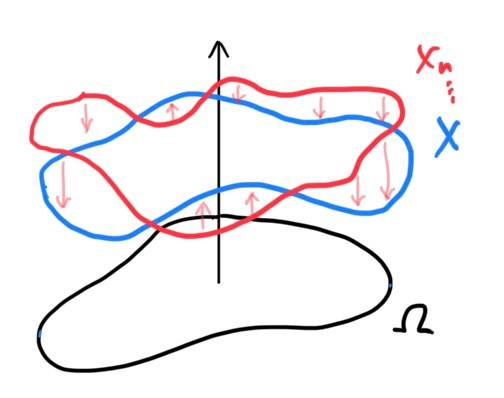
\includegraphics[scale=0.3]{img/sure_convergence.jpg}
\end{center}
\end{definition}

But this definition is too strong of a form of convergence, since in probability we don't care about values over sets of measure $0$. That is, if we have two probability distributions that differ from each other on a set of measure $0$, then they can be considered essentially the same probability distribution. 

\begin{definition}[Almost Sure Convergence of RVs]
The sequence of random variables $\{ X_n\}_{n \in \mathbb{N}}$ is said to \textbf{converge almost surely} or \textbf{converge with probability 1} to $X$ if $X_n (\omega) \rightarrow X (\omega)$ on a subset of probability $1$. That is, 
\[\mathbb{P} \big( \{ \omega \in \Omega \mid \lim_{n \rightarrow \infty} X_n (\omega) = X(\omega) \} \big) = 1\]
Considering small technicalities, it can be shown that this set of $\omega$'s can be considered an event in $\mathcal{F}$. This can be visualized similarly as sure convergence, but now the surfaces don't have to converge on sets of measure $0$. 
\begin{center}
    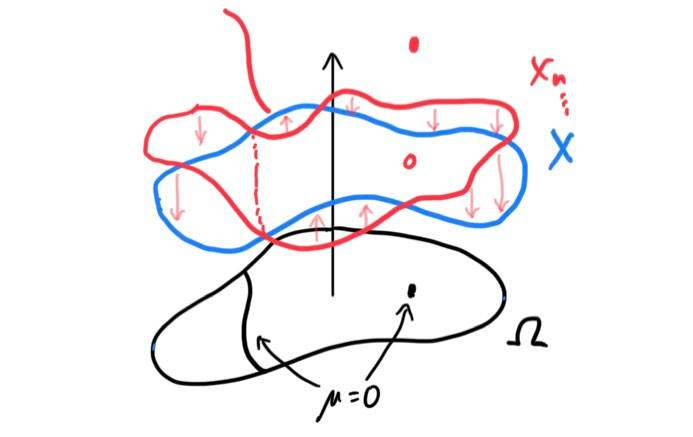
\includegraphics[scale=0.3]{img/almost_sure_convergence.jpg}
\end{center}
Crudely put, we just have to look at each $\omega \in \Omega$, see if $X_n (\omega)$ converges to $X(\omega)$ as $n \rightarrow \infty$, and determine if the set of all $\omega$'s that satisfy this have probability $1$. In other words, let us have some experiment with outcome space $\Omega$. With probability $1$, some $\omega \in \Omega$ will be realized, which will realize the sequence of realized random variables
\[X_1 (\omega), X_2 (\omega), X_3 (\omega), \ldots \]
that will converge to $X(\omega)$. Visually, we can imagine selecting a random point in $\Omega$, which will not hit the curve or point (with probability $1$), and in these cases, the sequence of points will converge to $X(\omega)$. 
\begin{center}
    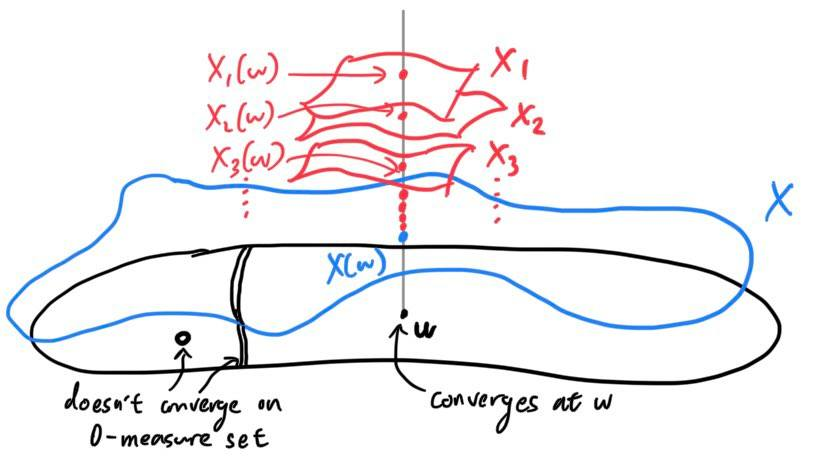
\includegraphics[scale=0.3]{img/almost_sure_convergence_2.jpg}
\end{center}
\end{definition}

\begin{definition}[Convergence in Probability]
The sequence of random variables $\{ X_i\}_{i \in \mathbb{N}}$ is said to \textbf{converge to $X$ in probability} if for all $\epsilon > 0$, 
\[\lim_{n \rightarrow \infty} \mathbb{P} \big( |X_n - X| > \epsilon \big) = 0\]
To understand what this means, fix an $\epsilon > 0$. Then, $X_1$ may be very far from $X$, meaning that the event $|X_1 - X| > \epsilon$, i.e. the set of all $\omega \in \Omega$ satisfying $|X_1(\omega) - X (\omega)| > \epsilon$ may be a larger portion of $\Omega$. Now, as we increase $n$, this event will become smaller (in the way that it's probability decreases) until it reaches $0$. 
\begin{center}
    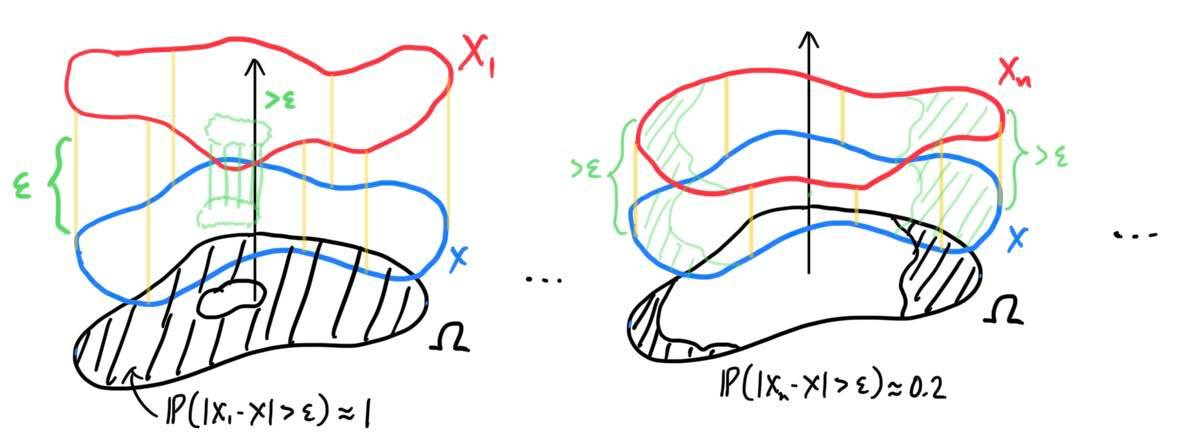
\includegraphics[scale=0.3]{img/convergence_in_probability.jpg}
\end{center}
\end{definition}

\begin{example}
Given $X_n \sim \mathrm{Exponential}(n)$ with $f_{X_n} (x) = n e^{-nx}$, we show that the sequence converges in probability to the $0$ random variable. Given $\epsilon > 0$, we have 
\begin{align*}
    \lim_{n \rightarrow \infty} \mathbb{P}(|X_n - 0| > \epsilon) & = \lim_{n \rightarrow \infty} \mathbb{P}(X_n > \epsilon \cup X_n < -\epsilon) \\
    & = \lim_{n \rightarrow \infty} \mathbb{P}(X_n > \epsilon) \\
    & = \lim_{n \rightarrow \infty} \int_\epsilon^\infty n e^{-nx} \,dx \\
    & = \lim_{n \rightarrow \infty} e^{-n \epsilon} = 0
\end{align*}
We can imagine this since given any small $\epsilon > 0$, we can see that increasing $n$ results in the distribution of $X_n$ to decrease at a faster rate, and thus a bigger portion of the distribution would lie within $\epsilon$ of the $0$ random variable. 
\begin{center}
    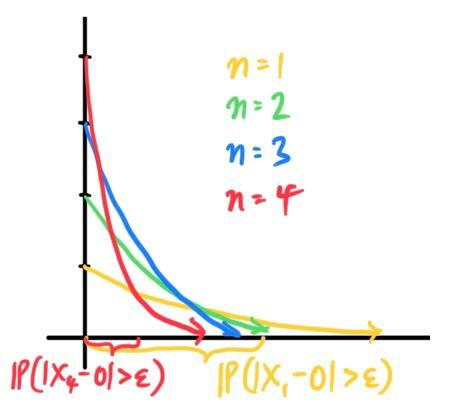
\includegraphics[scale=0.3]{img/convergence_in_prob_exponential.jpg}
\end{center}
\end{example}

\begin{definition}
We say $X_n$ \textbf{converges to $X$ in the $r$th mean} if 
\[\lim_{n \rightarrow \infty} \mathbb{E} \big[ |X_n - X|^r \big] = 0\]
For $r = 2$, $X_n$ is said to converge to $X$ in the \textbf{mean-squared sense}. 
\end{definition}

\begin{definition}[Convergence in Distribution]
We say $X_n$ \textbf{converges to $X$ in distribution} if the CDF of $X_n$ converges pointwise to the CDF of $X$, i.e. 
\[\lim_{n \rightarrow \infty} F_{X_n} (x) = F_X (x)\]
for all $x$ where $F_{X}$ is continuous. 
\end{definition}

So for practical purposes there are 5 notions of convergence that we will work with: 
\begin{enumerate}
    \item Sure convergence: $X_n \xrightarrow{p.w.} X$ 
    \item Almost sure convergence: $X_n \xrightarrow{a.s.} X$ 
    \item Convergence in probability: $X_n \xrightarrow{i.p.} X$ 
    \item Convergence in $r$th mean: $X_n \xrightarrow{rth} X$ (Mean square: $X_n \xrightarrow{m.s.} X$) 
    \item Convergence in distribution: $X_n \xrightarrow{D} X$
\end{enumerate}

\begin{theorem}[Hierarchy of Convergence]
The following implications hold: 
\begin{enumerate}
    \item Pointwise c. $\implies$ almost sure c. $\implies$ c. in probability $\implies$ c. in distribution. 
    \item $r$th mean c. $\implies$ c. in probability $\implies$ c. in distribution. 
\end{enumerate}
\end{theorem}

Trying to understand these relationships can be very hard, so we will take some time to do that, with some examples. First, convergence in distribution is clearly the weakest, since convergence in distribution does not imply that the random variables need be close to each other. Take a look at the random variables $X \sim \mathrm{Bernoulli}(1/2)$ and $Y = 1 - X$. $X$ and $Y$ are both $\mathrm{Bernoulli}(1/2)$ with the same distribution, but they are \textit{not} the same random variable since $X - Y = 1$ always. Therefore, we can think of two random variables that have the same distribution but are not "close" to each other as functions over $\Omega$ that divide it into identical, but differently cut, distributions. 
\begin{center}
    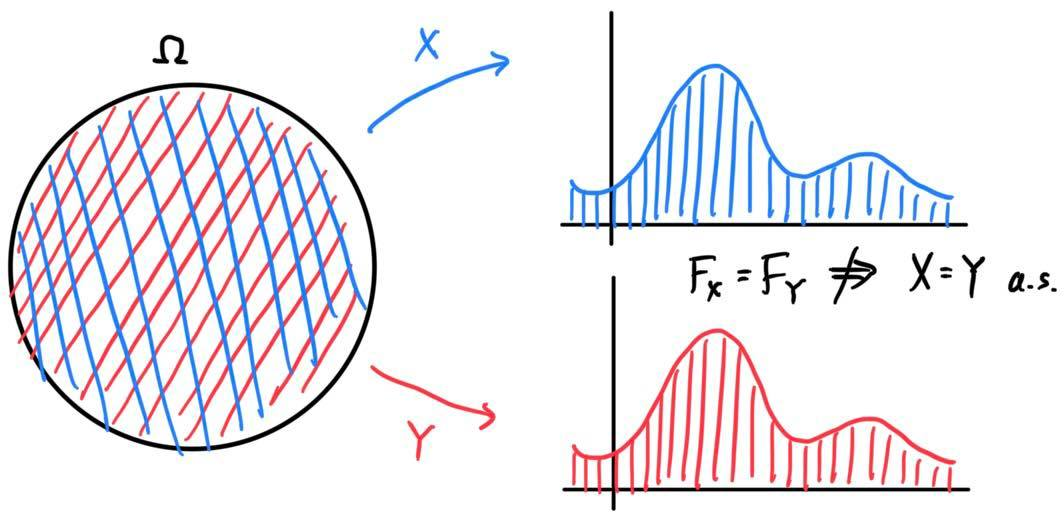
\includegraphics[scale=0.23]{img/prob_in_distribution.jpg}
\end{center}

\begin{example}[C. in Distribution $\centernot\implies$ C. in Probability]
Let $X_1, X_2, \ldots$ be such that $X_i = X$ for all $i$ where $X \sim \mathrm{Bernoulli}(1/2)$. This does not mean that the $X_i$'s are iid Bernoulli; they are all copies of the same $X$, i.e. forms a constant sequence. Let $Y = 1 - X$. Clearly, $X_n \xrightarrow{D} Y$ since the CDF of every $X_i$ is the same as that of $Y$, but $|X_n - Y| = 1$ for all $n$, so there is no convergence.  
\end{example}

\begin{example}[C. in Distribution $\centernot\implies$ C. in Probability]
Let $X_1, X_2, \ldots \sim \mathcal{N}(0, 1)$ and $Y = -X$. Then, by symmetry of the standard Gaussian, both $X$ and $Y$ have the same CDF, but they are not the same random variable: their signs are opposite. 
\end{example}

\subsubsection{Convergence in Probability vs Almost Surely} 

Convergence almost surely and convergence with probability are very different. Almost sure convergence has the limit inside the probability, which indicates that we are talking about convergence of a sequence of random variables. On the other hand, convergence in probability has the limit on the outside, which talks about convergence of a sequence of probabilities. But a key point is that almost sure convergence implies convergence in probability. It happens so because there could exist a subset of small probability in $\Omega$ where the $X_n$'s and $X$ need not be close, but the probabilities of them deviating over whole $\Omega$ is small. 

\begin{example}[C. in Probability $\centernot\implies$ C. Almost Surely]
Consider the interval $\Omega = [0, 1]$ and the subsets $A_1 = [0, 0.1], A_2 = [0.1, 0.2], \ldots$, such that at $A_{10} = [0.9, 1.0]$, the size with halve and will go to the left boundary, $A_{11} = [0, 0.05], \ldots$. Then, the sequence of indicator random variables 
\[X_n \coloneqq 1_{A_n}\]
looks like it's converging to the $0$ random variable. Indeed, $X_n \xrightarrow{i.p.} 0$ since the probability that $X_n$ deviates from $0$ by more than some small $\epsilon$ is simply the measure of $A_n$ itself, which decreases to $0$. That is, given some small $\epsilon > 0$, we have 
\[\lim_{n \rightarrow \infty} \mathbb{P} (|X_n - 0| > \epsilon) = \lim_{n \rightarrow \infty} \mathbb{P}(1_{A_n} > \epsilon ) = \lim_{n \rightarrow \infty} \mathbb{P}(A_n) = 0\]
Now let's show that this doesn't converge almost surely. For \textit{any} outcome $\omega \in \Omega$, the sequence of random variables $X_1(\omega), X_2(\omega), \ldots$ will hit these intervals $A_n$ infinitely many times and will not converge to $0$, since there will always be a $1$ down the sequence. They will occur with decreasing frequency but they will always occur. Therefore, with probability $1$, whatever realized sequence will not converge to the $0$ random variable. 
\end{example}

Here is another standard counterexample. 

\begin{example}[C. in Probability $\centernot\implies$ C. Almost Surely]
Let us take the sequence $X_1, X_2, \ldots$ of independent random variables where $X_n \sim \mathrm{Bernoulli}(1/n)$. That is, 
\[\mathbb{P}(X_n = 1) = \frac{1}{n} \text{ and } \mathbb{P}(X_n = 0) = 1 - \frac{1}{n}\]
So, as $n$ gets large we expect $X_n$ to realize values of $0$ more and more. Showing that $X_n \xrightarrow{i.p.} 0$ is easy, since we can compute for any $\epsilon > 0$
\begin{align*}
    \lim_{n \rightarrow \infty} \mathbb{P}(|X_n - 0| > \epsilon) & = \lim_{n \rightarrow \infty} \mathbb{P}(|X_n| > \epsilon) \\
    & = \lim_{n \rightarrow \infty} \mathbb{P}(X_n = 1) \\
    & = \lim_{n \rightarrow \infty} \frac{1}{n} = 0
\end{align*}
We want to show that this does not converge almost surely to $0$, i.e. there is some set of nonzero measure such that for some $\omega$ in that set, the sequence $X_1 (\omega), X_2(\omega), \ldots$ does not converge to $0$. This can be hard to see at first, but the fact that we have independence and the terms are $\frac{1}{n}$ hints at the Borel-Cantelli lemma. Let $A_n$ be the event that $\{X_n = 1\}$ (i.e. the preimage of the singleton set under $X_n$: $X_n^{-1} ( \{1\})$). Then, the $A_n$'s are independent, and 
\[\sum_{n=1}^\infty \mathbb{P}(A_n) = +\infty \]
By the Borel-Cantelli lemma 2, this implies that almost surely infinitely many $A_n$'s will occur. That is, we can choose as large of an $n$ as we like, go down the sequence until we look at $X_n, X_{n+1}, \ldots$, and we are guaranteed with probability $1$ that at least one of the $X_i$'s after $n$ will realize a $1$. This means that in every realization of $X_1, X_2, \ldots$, we will get a sequence of $0$s and $1$s, but since BCL states that no matter how far down the road you will always get at least another $1$, this sequence does not converge to $0$.  
\end{example}

The commonality between these two examples is that sequence of random variables satisfies convergence in probability as follows: As $n$ increases, $X_n$ is more and more likely to be near $X$ (in the way that $|X_n - X| < \epsilon$ for some $\epsilon > 0$), ultimately satisfying this closeness property with probability $1$ as $n \rightarrow \infty$. For example, we could have 
\begin{align*}
    \mathbb{P}(|X_1 - X| > \epsilon) & = 1 \\
    \mathbb{P}(|X_2 - X| > \epsilon) & = 1/2 \\
    \mathbb{P}(|X_3 - X| > \epsilon) & = 1/3 \\
    \ldots & = \ldots 
\end{align*}
This definitely satisfies convergence in probability, but this leaves open the possibility that $\mathbb{P}(|X_n - X| > \epsilon)$ an infinite number of times, although at infrequent intervals. Therefore, when looking at the sequence 
\[X_1, X_2, X_3, \ldots\]
each random variable \textit{individually} may have less chance of being more than $\epsilon$ away from $X$, but since there is an infinite number of them in the sequence, the sequence \textit{in totality} may contain an infinite number of cases where $|X_n - X| > \epsilon$. Convergence almost surely tells us that we are \textit{guaranteed} (with probability $1$) that this sequence will converge to $X$. That is, we can specify an $N \in \mathbb{N}$ such that $|X_n - X| < \epsilon$ for all $n > N$. 

Let us define some $\epsilon > 0$ and consider a sequence of random variables $\{X_n\}_{n \in \mathbb{N}}$. Given some outcome $\omega \in \Omega$, we will consider it a \textit{success} if $|X_n(\omega) - X(\omega)| < \epsilon$ and \textit{failure} if not. Then, convergence in probability tells us that the probability of failure goes to $0$ as $n$ goes to infinity and therefore we get better and better estimates of $X$. Convergence almost surely is a bit stronger and says that the total number of failures is \textit{finite}. That is, after a certain point $N$, the random variable $X_n$ will \textit{always} estimate $X$ within an error of $\epsilon$ (i.e. such that $|X_n - X| < \epsilon$). But since you don't know when you've exhausted all failures, there is not much of a difference from a practical point of view. 


\subsubsection{Complete Convergence}

When proving almost sure convergence, we'd ideally just look at all the $\omega \in \Omega$ where $X_n (\omega) \rightarrow X(\omega)$, and if this set has probability measure $1$, then we are done. But this is not very practical, so we use the following theorem, which gives a sufficient condition for $X_n \xrightarrow{a.s.} X$. 

\begin{theorem}
If for all $\epsilon > 0$, 
\[\sum_{n=1}^\infty \mathbb{P}(|X_n - X| > \epsilon ) < \infty\]
then $X_n \xrightarrow{a.s.} X$. This condition is a bit stronger, since not only are we saying that $\mathbb{P}(|X_n - X| > \epsilon)$ tends to $0$ as $n \rightarrow \infty$, but that it goes down fast enough to keep the series convergent. 
\end{theorem}
\begin{proof}
Let the event that $|X_n - X| > \epsilon$ be denoted $A_n (\epsilon)$ (i.e. the preimage of $(\epsilon, \infty)$ under the map $|X_n - X|$, which is a $\mathcal{F}$-measurable set). Since the sum of their probabilities is finite, by the Borel-Cantelli lemma 1, finitely many $A_n(\epsilon)$'s will occur with probability $1$. This means that for any $\epsilon > 0$, $|X_n - X| \leq \epsilon$ for all large enough $n$, meaning that it converges to $0$. 
\end{proof}

\subsection{Laws of Large Numbers}

\begin{theorem}[Weak Law of Large Numbers]
Let $X_1, X_2, ..., X_n$ be a sequence of iid random variables, with finite mean $\mathbb{E}[X]$. Then, the average of the random variables $S_n / n$ converges in probability to $\mathbb{E}[X]$. 
\[\frac{S_n}{n} = \frac{1}{n} \sum_{i=1}^n X_i \xrightarrow{i.p} \mathbb{E}[X]\]
That is, for any $\epsilon > 0$, 
\[\lim_{n \rightarrow \infty} \mathbb{P} \bigg( \bigg| \Big( \frac{1}{n} \sum_{k=1}^n X_k \Big) - \mathbb{E}[X] \bigg| > \epsilon \bigg) = 0\]
\end{theorem}
\begin{proof}
We first do the proof assuming additionally that $X$ has finite variance, so $\mathrm{Var}[X] < \infty$. We will show that the random variable $S_n/n$ converges in mean square to $\mathbb{E}[X]$, which will imply convergence in probability. Note that $\mathbb{E}[S_n / n] = \mathbb{E}[X]$, and 
\begin{align*}
    \lim_{n \rightarrow \infty} \mathbb{E} \bigg[ \bigg| \frac{S_n}{n} - \mathbb{E}[X] \bigg|^2 \bigg] & = \lim_{n \rightarrow \infty} \mathbb{E} \bigg[ \bigg| \frac{S_n}{n} - \mathbb{E}\Big[\frac{S_n}{n}\Big] \bigg|^2 \bigg] \\
    & = \lim_{n \rightarrow \infty} \mathrm{Var}\Big( \frac{S_n}{n} \Big) \\
    & = \lim_{n \rightarrow \infty} \frac{\mathrm{Var}(S_n)}{n^2} \\
    & = \lim_{n \rightarrow \infty} \frac{\mathrm{Var}[X]}{n} = 0
\end{align*}
\end{proof}

\begin{theorem}[Strong Law of Large Numbers]
Let $X_1, X_2, ..., X_n$ be a sequence of iid random variables, with finite mean $\mathbb{E}(X_k)$ and with finite variance. Then, the average of the random variables $S_n / n$ converges almost surely to $\mathbb{E}[X]$. 
\[\frac{S_n}{n} \xrightarrow{a.s.} \mathbb{E}[X]\]
That is, 
\[\mathbb{P} \bigg( \Big\{ \omega \in \Omega \mid \lim_{n \rightarrow \infty} \Big( \frac{1}{n} \sum_{i=1}^n X_i (\omega) \Big) = \mathbb{E}[X] \Big\} \bigg) = 1\]
\end{theorem}

Now let's compare these two laws. They both deal with averages of random variables, i.e. we keep sampling from $X$ and compute the averages $\overline{X}_n$. The weak law states that for a specified large $n$, the average $\overline{X}_n$ is likely to be near $\mathbb{E}[X]$. But it leaves open the possibility that $|\overline{X}_n - \mathbb{E}[X]| > \epsilon$ happens an infinite number of times (although less frequently). So no matter how big of an $n$ we choose, there could always be an $\overline{X}_n$ in the future that fails to satisfy $|\overline{X}_n - \mathbb{E}[X]| > \epsilon$. However, the strong law shows that this almost surely will not occur. That is, with probability $1$, we have for any $\epsilon > 0$ the inequality $|\overline{X}_n - \mathbb{E}[X]| < \epsilon$ for all large enough $n$ greater than a certain $N$. Note that the weak law does not guarantee the existence of such an $N$. 

This result is very useful because it justifies experiments that estimate some value by taking averages. 

\begin{example}[Estimating Speed of Light]
Say that we are conducting an experiment to justify the speed of light, which will have true value $\mu$. The laws of large numbers say that in theory, after obtaining enough data, we can get arbitrarily close to the true speed of light. Choose $\epsilon > 0$ arbitrarily small. We can obtain $n$ estimates $X_1, \ldots, X_n$ of the speed of light and compute the average 
\[\overline{X}_n = \frac{1}{n} \sum_{i=1}^n X_i\] 
As we obtain more data, we can compute $\overline{X}_n$ for each $n = 1, 2, \ldots$. The weak law says that $\mathbb{P}(|\overline{X}_n - \mu| > \epsilon) \rightarrow 0$ as $n \rightarrow \infty$, i.e. the probability of our estimate being off by more than $\epsilon$ goes to $0$ (though it may happen with nonzero probability if we consider the infinite sequence). The strong law says that the number of times $|\overline{X}_n - \mu|$ is greater than $\epsilon$ is finite (with probability $1$), and after a certain point our estimates will perfectly lie within the error $\epsilon$. This gives us considerable confidence in the value $\overline{X}_n$ because it guarantees the existence of some $N \in \mathbb{N}$ s.t. $|\overline{X}_n - \mu| < \epsilon$ for all $n > N$, i.e. the average \textit{never} fails for $n > N$. 
\end{example}

\subsection{Concentration Inequalities}

Concentration inequalities give you probability bounds on random variables taking atypical values. For example, given a random variable with certain mean and variance, the probability of that random variable taking values outside a certain range around the mean is very small. It's called concentration because the probability concentrates around a certain range. 

The basic question here is that we would like to model a random variable $X$ over a probability space $\Omega$ and have some data $X_1, X_2, \ldots, X_n$ iid according to $X$. Let us have a fixed function $f: \mathbb{R}^n \longrightarrow \mathbb{R}$ that transforms the joint random variable $(X_1, \ldots, X_n)$ to create a new scalar RV 
\[f(X_1, \ldots, X_n) = f \circ (X_1, \ldots, X_n) : \Omega \longrightarrow \mathbb{R}\]
$f(X_1, \ldots, X_n)$ is a random variable so it has a mean, denote it $\mathbb{E}[f]$. Then concentration generally refers to the probability that the value of $f$ is at least some distance further from its mean. 
\[\mathbb{P} \big( |f(x) - \mathbb{E}[f] | \geq t \big) \leq \epsilon\]
for some small positive $\epsilon$. Usually, we would like this $\epsilon$ to be an exponentially decaying function of $t$ so that the bound goes down fast. This is what's so great about the Gaussian, which is why we'll introduce it here. 

\begin{theorem}[Gaussian Tail Inequality]
Given $X \sim \mathcal{N}(0, 1)$, the inequality says that the probability of $X$ taking values past a certain $t$ decays exponentially. 
\[\mathbb{P} \big( |X| > t \big) \leq \frac{2 e^{-t^2/2}}{t}\]
If we have $X_1, \ldots, X_n \sim \mathcal{N}(0, 1)$, then 
\[\mathbb{P} \big( |\overline{X}| > t \big) \leq \frac{2}{\sqrt{n} t} e^{-n t^2/2}\]
We can assume that the coefficient is less than $1$ if $n$ is large. The above tells us that this bound exponentially decays with $t$ but also with the number of samples $n$. 
\end{theorem}
\begin{proof}
We can simply check 
\[\phi(s) = \frac{1}{\sqrt{2\pi}} e^{-s^2/2} \implies \phi^\prime (s) = s \, \phi(s)\]
and use this to evaluate
\begin{align*}
    \mathbb{P}(X > t ) & = \int_t^\infty \phi(s) \,ds \\
    & = \int_t^\infty \frac{s}{s} \phi(s) \,ds \\
    & < \frac{1}{t} \int_t^\infty s \phi(s)\,ds \\
    & = \frac{1}{t} \int_t^\infty \phi^\prime (s)\,ds \\
    & = \frac{\phi(t)}{t}
\end{align*}
\end{proof}

Due to the exponential nature of the probability bound, we are extremely confident in getting the majority of our samples from a small interval. If we had taken some distribution like a Cauchy, with PDF of form 
\[f(x) \propto \frac{1}{1 + x^2}\]
Then we see that even though the shape looks like a Gaussian at first glance, the fat tails go down at the rate of $1/x^2$. It turns out that due to this, when we sample numerically, we occasionally get extreme values. 

\begin{theorem}[Markov's Inequality]
If $X$ is a non-negative random variable of finite expectation and $\alpha > 0$, then 
\[\mathbb{P}(X > \alpha) \leq \frac{\mathbb{E}[X]}{\alpha}\]
That is, the probability that $X$ takes a value greater than $\alpha$ is at most the expectation of $X$ divided by $\alpha$. This is meaningful only when $\mathbb{E}[X] < \alpha$, since otherwise the RHS will be greater than $1$.  
\end{theorem}

\begin{proof}
Given any $\alpha > 0$, we can set 
\[X = X \cdot 1_{X \leq \alpha} + X \cdot 1_{X > \alpha}\]
and by linearity, 
\begin{align*}
    \mathbb{E}[X] & = \mathbb{E}[X \cdot 1_{X \leq \alpha} + X \cdot 1_{X > \alpha}] \\
    & \geq \mathbb{E}[ X \cdot 1_{X > \alpha}] \\
    & \geq \alpha \mathbb{E}[1_{X > \alpha}] \\
    & = \alpha \, \mathbb{P}(X > x) 
\end{align*}
\end{proof}

In other words, the probability that $X > \alpha$ goes down at least as fast as $1/\alpha$. For example, setting $\alpha = 2 \mathbb{E}[X]$, the probability that $X$ takes value that is at least twice its expectation is at most $1/2$. Furthermore, as $X$ gets very large, the probability that it will take a value beyond a large $\alpha$ goes down faster than $1/\alpha$. But this is a very conservative inequality, and usually the probability goes down much faster. 

Markov's inequality is very conservative but very general, too. If we make further assumptions about the random variable $X$, we can often make stronger bounds. Chebyshev's inequality assumes a (possibly negative) random variable with finite variance and states that the probability will go down as $1/x^2$. 

\begin{theorem}[Chebyshev Inequality]
Given (possibly negative) random variable $X$, if $\mathbb{E}[X] = \mu < +\infty$ and $\Var(X) = \sigma^2 < +\infty$, then for all $\alpha > 0$, 
\[\mathbb{P} \big( |X - \mu| > k \sigma \big) \leq \frac{1}{k^2} \iff \mathbb{P}(|X - \mu| > \alpha) \leq \frac{\mathrm{Var}[X]}{\alpha^2}\]
That is, the probability that $X$ takes a value further than $k$ standard deviations away from $\mu$ goes down by $1/k^2$. Therefore, if $\sigma$ is small, then this bound will be small since there is more concentration in the mean. 
\end{theorem}
\begin{proof}
We apply Markov's inequality to the non-negative random variable $|X - \mu|$. 
\[\mathbb{P}(|X - \mu| > \alpha) = \mathbb{P}(|X - \mu|^2 > \alpha^2) \leq \frac{\mathbb{E}(|X - \mu|^2)}{\alpha^2} = \frac{\mathrm{Var}[X]}{\alpha^2}\]
since the numerator on the RHS is the definition of variance. 
\end{proof}

Chebyshev inequality is just Markov's inequality applied to $X^2$ (assuming $0$ mean), and often yields a better bound. But even Chebyshev's inequality turns out to be quite loose, and even this $1/k^2$ is not a very nice bound. We could apply Markov's inequality to higher powers of $X$, e.g. given a random variable $X$, we can apply Markov's inequality to the $k$th power of nonnegative random variable $|X - \mathbb{E}[X]|$: 
\[\mathbb{P} (|X - \mathbb{E}[X] | > \alpha) = \mathbb{P}\big( |X - \mathbb{E}[X] |^k > \alpha^k \big) \leq \frac{\mathbb{E}( |X - \mathbb{E}[X] |^k )}{\alpha^k}\]
The natural culmination of all this is to apply Markov's inequality to $e^X$ (or, for a little flexibility, $e^{t X}$, where $t$ is a constant to be optimized). This gives us an exponential bound on $\mathbb{P}(X > \alpha)$. 

\begin{example}[Gaussian]
For the normal distribution, recall the 67-95-99.7 rule. It is well known that the probability of a random variable taking values within $2$ standard deviations from the mean is 95\%, so the probability that it takes outside is 5\%, or $1/20$, which is less than the $1/2^2 = 1/4$ bound given by Chebyshev. 
\end{example}

\subsubsection{Chernoff Bound and MGFs}

\begin{theorem}[Chernoff Bound]
Given a (possibly negative) random variable $X$, assume that its moment generating function $M_X (s) = \mathbb{E}[e^{s X}]$ is finite for every $s \in [-\epsilon, \epsilon]$. Then, since $x \mapsto e^{s x}$ is monotonically increasing, we have the identity 
\[\mathbb{P}(X > \alpha) = \mathbb{P}(e^{s X} > e^{s \alpha}) \text{ for } s > 0\]
But since the new random variable $e^{s X}$ is nonnegative, we can now go back to Markov inequality and write 
\[\mathbb{P}(X > \alpha) = \mathbb{P}(e^{s X} > e^{s \alpha}) \geq \frac{\mathbb{E}[e^{s X}]}{e^{s \alpha}} = M_X (s) \, e^{-s \alpha}\]
for $s > 0$ (for identity above to hold) \textit{and} $s \in D_X$ (and it is in domain of convergence). Now, we have an exponentially decaying bound in terms of $\alpha$. We have the freedom to choose $s$, since our bound is in terms of $\alpha$, so we must choose $s$ that minimizes $M_X (s) \, e^{-s \alpha}$. Ultimately, our best bound is 
\[\mathbb{P}(X > \alpha) \leq \inf_{s > 0} M_X (s) \, e^{-s \alpha}\]
After we optimize over $s$ what remains on the RHS is a function of $\alpha$. 
\end{theorem}

Now, we can calculate the MGF of $X$ directly if we knew the distribution of $X$, but we can also get bounds on it given some coarse statistics of $X$. 

\begin{lemma}
Let $X$ be a $0$-mean random variable s.t. $a \leq X \leq b$ with probability $1$. Then for all $t > 0$, 
\[\mathbb{E}[ e^{t X}] \leq e^{t^2 (b - a)^2 / 8}\]
\end{lemma}
\begin{proof}
We can write $x = \lambda a + (1 - \lambda b)$, $0 \leq \lambda \leq 1$, and convexity of the exponential tells us that 
\[e^{tx} \leq \lambda e^{ta} + (1 - \lambda) e^{tb}\]
Plugging in $\lambda = (b - x) / (b - a)$ then gives 
\[e^{tx} \leq \frac{b - x}{b - a} e^{tx} + \frac{x - a}{b - a} e^{tb} \]
Take expectations of both sides, and using linearity of expectation and the fact that $\mathbb{E}[X] = 0$. 
\[\mathbb{E}[e^{tX}] \leq \frac{b - \mathbb{E} X}{b - a} e^{ta} + \frac{\mathbb{E} X - a}{b - a} e^{tb} = \frac{b e^{ta} - a e^{tb}}{b - a} \leq e^{t^2 (b - a)^2 / 8}\]
\end{proof}

\subsubsection{Hoeffding's Inequality}

Hoeffding's inequality is one of the most important inequalities in concentration of measure. The proof of this inequality involves many useful tricks. 

\begin{theorem}[Hoeffding's Inequality]
Let $X_1, X_2, \ldots, X_n$ be independent (not necessarily identical) random variables s.t. $a_i \leq X_i \leq b_i$ almost surely. Consider the random variable $\overline{X} = \frac{1}{n} (X_1 + \ldots + X_n)$. Then, for all $t > 0$, we have the two inequalities
\begin{align*}
    \mathbb{P}\big( \overline{X} - \mathbb{E}[\overline{X}] \geq t \big) & \leq \exp \bigg( -\frac{2 n^2 t^2}{\sum_{i=1}^n (b_i - a_i)^2} \bigg) \\
    \mathbb{P}\big( \overline{X} - \mathbb{E}[\overline{X}] \leq -t \big) & \leq \exp \bigg( -\frac{2 n^2 t^2}{\sum_{i=1}^n (b_i - a_i)^2} \bigg)
\end{align*}
which can be combined to produce 
\[\mathbb{P}\big( \big| \overline{X} - \mathbb{E}[\overline{X}] \big| \geq t \big) \leq 2 \exp \bigg( -\frac{2 n^2 t^2}{\sum_{i=1}^n (b_i - a_i)^2} \bigg)\]
We can create an equivalent bound on the sum $S_n = X_1 + \ldots + X_n$: 
\begin{align*}
    \mathbb{P}\big(| S_n - \mathbb{E}[S_n] | \geq t\big) & = \mathbb{P}\big( n |\overline{X} - \mathbb{E}[\overline{X}] | \geq t \big) \\
    & = \mathbb{P} \big( |\overline{X} - \mathbb{E}[X] | \geq \frac{t}{n} \big) \\
    & \leq 2 \exp \bigg( -\frac{2 t^2}{\sum_{i=1}^n (b_i - a_i)^2} \bigg) 
\end{align*}
\end{theorem}
\begin{proof}
We will prove just with the case where $X_1, \ldots X_n$ are all bounded by $[a, b]$, which gives 
\[\mathbb{P} \big( |\overline{X} - \mathbb{E}[\overline{X}] | \geq t \big) \leq 2 \exp \bigg( - \frac{2 n t^2}{(b - a)}\bigg)\] 
Now, we can write 
\begin{align*}
    \mathbb{P}(\overline{X}_n > \epsilon ) & = \mathbb{P} \Big( \sum_{i=1}^n X_i \geq n \epsilon \Big) \\
    & = \mathbb{P} \big( e^{t \sum X_i} \geq e^{t n \epsilon} \big) & (\text{Variational Technique}) \\
    & \leq e^{- t n \epsilon} \, \mathbb{E}[e^{t \sum X_i}] & (\text{Markov's Inequality}) \\
    & = e^{-t n \epsilon} \, \big( \mathbb{E}[ e^{t X_i}] \big)^n & (\text{Independence}) \\
    & \leq e^{-t n \epsilon} e^{n \frac{t (b - a)^2}{2}} & (\text{prev. lemma}) 
\end{align*}
The step where we introduce an extra parameter $t$ is called a variational technique, used for optimization, and we can adjust $t$ to make it as small as possible. Taking the derivative of the final expression w.r.t. $t$ and solving for $0$ gives us $t = \frac{4 \epsilon}{(b - a)^2}$, and substituting into the expression gives the bound as 
\[\mathbb{P}(\overline{X}_n > \epsilon ) \leq \exp \bigg(- \frac{2 n \epsilon^2}{(b - a)^2}\]
\end{proof}

By further rearranging, we can write it as 
\[\mathbb{P} \bigg( | \overline{X} - \mathbb{E}[\overline{X}] | \geq t \sqrt{\frac{\sum_{i=1}^n (b_i - a_i)^2}{n^2}} \bigg) \leq 2 \exp(-2t^2)\]
which now looks like our Chebyshev inequality, but without a notion of standard deviation. But note the fact if $a_i \leq X_i \leq b_i$, then $\mathrm{Var}(X_i) \leq (b_i - a_i)^2$ (since $\mathrm{Var}(X_i) = \mathbb{E}[(X_i - \mathbb{E}[X_i])^2] \leq \mathbb{E}[(b_i - a_i)^2]$). So, we have 
\[\mathrm{Var}(\overline{X}) \leq \frac{\sum_{i=1}^n (b_i - a_i)^2}{n^2} \implies \mathbb{P}\bigg( |\overline{X} - \mathbb{E}[\overline{X}] | \geq t \sqrt{\frac{\sum_{i=1}^n (b_i - a_i)^2}{n^2}} \geq \mathrm{Var}(\overline{X}) \bigg) \leq 2\exp(-2t^2)\]
which allows us to interpret Hoeffding's inequality in a more familiar way. It says that the probability that the sample average is more than $t$ standard deviations from its expectation is at most $2 e^{-2t^2}$. 

\begin{corollary}
If $X_1, X_2, \ldots, X_n$ are independent with $\mathbb{P}(a_i \leq X_i \leq b_i) = 1$ and common mean $\mu$, then 
\[\mathbb{P}\bigg[ \big| \overline{X}_n - \mu \big| \leq \sqrt{ \frac{\sum_{i=1}^n (b_i - a_i)^2}{2n^2} \log \Big(\frac{2}{\delta}\Big)} \bigg] \geq 1 - \delta\]
\end{corollary}

\begin{example}[Bernoulli]
Applying Hoeffding's inequality to a sequence of $n$ $p$-coin tosses $X_1, \ldots, X_n \sim \mathrm{Bernoulli}(p)$ gives 
\[\mathbb{P}\big( | \overline{X}_n - p | > \epsilon \big) \leq 2 \exp^{-2 n \epsilon^2}\]
\end{example}

\begin{example}[Mean]
Suppose we have $X_1, X_2, \ldots X_n \sim \mathrm{Bernoulli}(p)$, all iid. Then, by Hoeffding's inequality, the average $\overline{X} = \frac{1}{n} (X_1 + \ldots + X_n)$ is tightly concentrated around $p$. 
\[\mathbb{P} \big( | \overline{X} - p | \geq t \big) \leq 2 e^{-2 n t^2}\]
Note that $b_i - a_i = 1 - 0 = 1$ for all $i$. There is an exponential decay in the probability of the sample mean deviating from its expectation. 
\end{example}

\begin{example}[Hypercube]
  Pick $X \in [-1, +1]^d$ uniformly at random, i.e. choose iid $X_1,\ldots, X_d \sim \mathrm{Uniform}[-1, +1]$. The expectation is 
  \[\mathbb{E} ||X||^2 = \sum_{i=1}^d \mathbb{E} X_i^2 = \sum_{i=1}^d \int_{-1}^1 x^2 f_X (x) \,dx = \sum_{i=1}^d \int_{-1}^1 \frac{1}{2} x^2 \,dx = \frac{d}{3}\]
  Then, it can be shown that $||X|| = $ is tightly concentrated around $\sqrt{d/3}$. We show this again with Hoeffding's inequality by showing the concentration of $||X||^2$ around $d/3$. 
  \[\mathbb{P} \bigg( \bigg| ||X||^2 - \frac{d}{3} \bigg| \geq t \bigg) \leq 2 \exp \Big( - \frac{ d t^2}{2} \Big)\]
  This tells us that if we choose the uniform random vector $X \in [-1, +1]^d$, the vast majority of our samples will have $||X|| \approx \sqrt{d/3}$. 
\end{example}


Hoeffding's inequality does not use any information about the random variables expect for the fact that they are bounded. If the variance of $X_i$ is small, then we can get a sharper inequality from Bernstein's inequality. 

\begin{theorem}[Bernstein's Inequality]
If $\mathbb{P}(|X_i| \leq c) = 1$ and $\mathbb{E}[X_i] = 0$, set $\overline{X} = \frac{1}{n} \sum_{i=1}^n X_i$. Then, for any $t > 0$, 
\[\mathbb{P} \big( \big| \overline{X} \big| > \epsilon \big) \leq 2 \exp \bigg( - \frac{n \epsilon^2}{2 \sigma^2 + 2 c \epsilon /3} \bigg)\]
where $\sigma^2 = \frac{1}{n} \sum_{i=1}^n \mathrm{Var}(X_i)$. 
\end{theorem}

\subsubsection{Concentration of Lipshitz Functions}

Observing the Hoeffding bound, one might wonder whether such concentration applies only to averages or sums of random variables. After all, what's so special about averages? It turns out that the relevant feature of the average that yields tight concentration is that it is smooth in the way that if we change the value of one random variable the function does not change dramatically. 

\begin{theorem}[Bounded Difference Inequality]
Let has have independent random variables $X_1, X_2, \ldots, X_n$ and a function $f: \mathbb{R}^n \longrightarrow \mathbb{R}$ that satisfies the \textbf{bounded difference property} that 
\[\big| f(x_1, \ldots, x_k, \ldots, x_n) - f(x_1, \ldots, x_k^\prime, \ldots, x_n) \big| \leq c_k\]
for every $x, x^\prime \in \mathbb{R}^n$. That is, the function changes by at most $c_k$ if its $k$th coordinate is changed. Then, for all $t \geq 0$, we have the concentration inequality: 
\begin{align*}
    \mathbb{P} \big( f(X_1, \ldots, X_n) - \mathbb{E}[ f(X_1, \ldots, X_n)] \geq t \big) & \leq \exp \bigg(- \frac{2t^2}{\sum_{k=1}^n c_k^2} \bigg) \\
    \mathbb{P} \big( f(X_1, \ldots, X_n) - \mathbb{E}[ f(X_1, \ldots, X_n)] \leq -t \big) & \leq \exp \bigg(- \frac{2t^2}{\sum_{k=1}^n c_k^2} \bigg)
\end{align*}
Combining the two gives 
\[\mathbb{P} \big( \big| f(X_1, \ldots, X_n) - \mathbb{E}[ f(X_1, \ldots, X_n)] \geq t \big| \big) \leq \exp \bigg(- \frac{2t^2}{\sum_{k=1}^n c_k^2} \bigg)\]
\end{theorem}

In fact, any smooth function of bounded independent random variables is tightly concentrated around its expectation, and the notion of smoothness is Lipshitz continuity. 

\begin{definition}
A function $f: \mathbb{R}^n \longrightarrow \mathbb{R}$ is $L$-Lipschitz w.r.t. the $l_p$-metric if for all $\mathbf{x}, \mathbf{y} \in \mathbb{R}^n$, 
\[|f(\mathbf{x}) - f(\mathbf{y})| \leq L ||\mathbf{x} - \mathbf{y}||_p\]
\end{definition}

\begin{example}
For $x = (x_1, x_2, \ldots, x_n)$, we define the average $a(x) = \frac{1}{n} (x_1 + \ldots + x_n)$. Then, $a$ is $(1/n)$-Lipschitz w.r.t. the $l_1$ metric, since for any $\mathbf{x}, \mathbf{y}$, 
\begin{align*}
    |a(\mathbf{x}) - a(\mathbf{y})| & = \bigg| \frac{1}{n} \big[ (x_1 - y_1) + \ldots + (x_n - y_n) \big] \bigg| \\
    & = \frac{1}{n} \big( |x_1 - y_1| + \ldots + |x_n - y_n| \big) \\
    & = \frac{1}{n} ||\mathbf{x} - \mathbf{y} ||_1
\end{align*}
\end{example}

It turns out that Hoeffding's bound holds for all Lipschitz functions w.r.t. the $l_1$ metric. 

\begin{theorem}
Suppose $X_1, X_2, \ldots, X_n$ are independent and bounded with $a_i \leq x_i \leq b_i$. Then, for any $f: \mathbb{R}^n \longrightarrow \mathbb{R}$ that is $L$-Lipschitz w.r.t. the $l_1$-metric, we have 
\begin{align*}
    \mathbb{P} [ f \geq \mathbb{E}(f) + t] & = \mathbb{P} [ f - \mathbb{E}(f) \geq t] \leq \exp\bigg(- \frac{2 t^2}{L^2 \sum_{i=1}^n (b_i - a_i)^2} \bigg) \\
    \mathbb{P} [ f \leq \mathbb{E}(f) - t] & = \mathbb{P} [ f - \mathbb{E}(f) \leq -t] \leq \exp\bigg(- \frac{2 t^2}{L^2 \sum_{i=1}^n (b_i - a_i)^2} \bigg)
\end{align*}
and combining these inequalities gives 
\[\mathbb{P} [ |f - \mathbb{E}(f)| \geq t] \leq \exp\bigg(- \frac{2 t^2}{L^2 \sum_{i=1}^n (b_i - a_i)^2} \bigg)\]
\end{theorem}

\subsection{Central Limit Theorem}

By the law of large numbers, the sample averages converge almost surely (and therefore converge in probability) to the expected value $\mu$ as $n \rightarrow \infty$. The CLT describes the size and the distributional form of the stochastic fluctuations around $\mu$ during this convergence. That is, it states that as $n$ gets larger, the distribution of the difference $\overline{X}_n - \mu$ approximates a $\mathcal{N}(0, \sigma^2 / n)$ distribution, where $\sigma^2$ is the variance of $X$. 


Roughly speaking, the (weak) law of large numbers says that 
\[\frac{S_n - n \mathbb{E}[X]}{n} \xrightarrow{i.p.} 0\]
That is, if we consider the sequence of functions $\{S_n - n \mathbb{E}[x]\}_{n \in \mathbb{N}}$, this sequence is sublinear (i.e. is $o(n)$). CLT does two things: 
\begin{enumerate}
    \item It specifically quantifies this fluctuation $\{S_n - n \mathbb{E}[X]$ by saying that it is approximately of order $\sqrt{n}$. 
    \item Furthermore, this fluctuation, when divided by $\sqrt{n}$ converges in distribution to a Gaussian. 
    \[\frac{S_n - n \mathbb{E}[X]}{\sqrt{n}} \xrightarrow{D} \mathcal{N}(0, \sigma_X^2)\]
\end{enumerate}

\begin{theorem}[Central Limit Theorem]
Let $X_1, X_2, X_3, ...$ be a sequence of iid random variables, with mean $\mu = \mathbb{E}[X]$ and with variance $\Var(X) = \sigma^2 < \infty$. Then, the sequence of random variables $\{\overline{X}_n\}_{n \in \mathbb{N}}$ converges in distribution to a Gaussian $\mathcal{N}(\mu, \sigma^2 / n)$. That is, 
\[\frac{\overline{X}_n - \mu}{\sigma \sqrt{n}} \xrightarrow{D} \mathcal{N}(0, 1)\]
\end{theorem}
\begin{proof}
Let $Z_i = \frac{X_i - \mu}{\sigma}$ and let $U_n = \frac{1}{\sqrt{n}} \sum_{i=1}^n Z_i$ (we can normalize the $X_i$'s since they have finite mean and variance). Note that since we have finite second moments 
\begin{align*}
    & \mathbb{E}[Z_i] = 0 < \infty \\
    & \mathrm{Var}[Z_i] = \mathbb{E}[ (Z_i - \mathbb{E}[Z_i])^2] = \mathbb{E}[Z_i^2] = 1 < \infty 
\end{align*}
we can Taylor expand the characteristic function $\varphi_{Z_i} (t)$ up to at least the second order (from moment generating property theorem). So, we have 
\begin{align*}
    \varphi_{Z_i} (t) & = 1 + \frac{\mathbb{E}[Z_i]}{1!} (i t)^1 + \frac{\mathbb{E}[Z_i^2]}{2!} (i t)^2 + o (t^2) \\
    & = 1 + 0 + \frac{1}{2} (i t)^2 + o (t^2) \\
    & = 1 - \frac{1}{2} t^2 + o(t^2) 
\end{align*}
Now calculate the CF of $U_n$. Since the $Z_i$'s are iid, we can get 
\[\varphi_{U_n} (t) = \Big( \varphi_{Z_i} \big( \frac{t}{\sqrt{n}} \big) \Big)^n = \Big( 1 - \frac{t^2}{2n} + o \big( \frac{t^2}{n} \big) \Big)^n\]
The $o(t^2 / n)$ term vanishes as $n \rightarrow \infty$, and using the limit $e^x = \lim_{n \rightarrow \infty} \big( 1 + \frac{x}{n} \big)^n$, we have 
\[\lim_{n \rightarrow \infty} \varphi_{U_n} (t) = \lim_{n \rightarrow \infty} \Big( 1 - \frac{t^2}{2n} + o \big( \frac{t^2}{n} \big) \Big)^n = e^{-t^2 / 2}\]
which is precisely the CF of a standard Gaussian random variable. Since CFs are unique, our result is proven. Essentially, we have proved convergence in distribution of random variables by showing convergence of their characteristic functions. 
\end{proof}

A big misconception is that this normalized sum has PDF that converges to a bell curve. It is the CDF (by definition of convergence in distribution) that converges to that of a Gaussian. That way, we can state this for discrete, continuous, mixtures: doesn't matter. They don't even need to have a density, since if we just took a bunch of Bernoulli's, the PMF of their sum would never be defined for an irrational number like $\pi$. But it would be defined for the CDF, and even though the CDF of a discrete random variable will have jumps, these jumps would get smaller and smaller until it converges pointwise. Even if the $X_i$'s had densities, the CLT does not say that their mean converges to the PDF of a normal. Just because the CDF converges, it doens't mean the PDF will look similiar. 

It also turns out (?) that we can use CLT to prove the weak law of large numbers, since (roughly speaking) as $n$ increases, the distribution of $\overline{X}_n$ concentrates more and more around $\mu$, and therefore the probability of $|\overline{X}_n - \mu| < \epsilon$ tends to $1$. 

\section{Conditional Expectation}

Conditional expectation is extremely important, especially in the context of stochastic processes, which is talked about in more detail in another set of notes. 

First, note that when we talk about the probability of event $A$ happening, or equivalently, the probability of $\omega \in A$, we can write this as the expected value of the indicator function $A$. 
\[\mathbb{P}(A) = \mathbb{E}[1_A]\]
This will come in handy later in connecting conditional probability and expectation. 

Now conditional expectation is quite tricky to understand at first. We will start by defining it given a $\sigma$-algebra and then given a random variable. 

\begin{definition}[Conditional Expectation]
Given a probability space $(\Omega, \mathcal{F}, \mathbb{P})$, a sub-$\sigma$-algebra $\mathcal{G} \subset \mathcal{F}$, and an $\mathcal{F}$-measurable random variable $X$ (with $\mathbb{E}[X] < \infty$), the \textbf{conditional expectation of $X$ given $\mathcal{G}$} is defined to be the $\mathcal{G}$-measurable random variable $Y = \mathbb{E}[X \mid \mathcal{G}]$ satisfying 
\[\int_A X \,d\mathbb{P} = \int_A Y \,d \mathbb{P}\]
or equivalently, 
\[\mathbb{E}[X \cdot 1_A] = \mathbb{E}[Y \cdot 1_A]\]
for all $A \in \mathcal{G}$. Any $Y$ satisfying these two conditions is said to be a \textbf{version} of $\mathbb{E}[X \mid \mathcal{F}]$. The critical detail to note here is that the conditional expectation $Y$, has the same expected value as $X$ does, not over just the whole $\mathcal{G}$, but \textit{in every subset $G$ of $\mathcal{G}$}. 
\end{definition}

We state without proof that $\mathbb{E}[X \mid \mathcal{G}]$ exists and is almost surely unique. For now, we can interpret this as the best approximation of the $\mathcal{F}$-measurable $X$ with the $\mathcal{G}$-measurable $Y$. Here is a useful analogy. Say that we have some "fine" function $X$ defined on the interval $[0, 1]$ with a fine Borel $\sigma$-algebra $\mathcal{F}$. 
\begin{enumerate}
    \item If we are given some sub-$\sigma$-algebra $\mathcal{G}$ composed of $\emptyset, [0, 0.5], (0.5, 1], [0, 1]$, then $Y$ would be the step function defined constantly on these intervals. 
    \item If we are given a finer sub-$\sigma$-algebra $\mathcal{H}$ generated by $[0, 0.25), [0.25, 0.5), [0.5, 0.75), [0.75, 1]$, then this would give a $\mathcal{H}$-measurable function that is a better approximation of $X$. 
\end{enumerate}
\begin{center}
    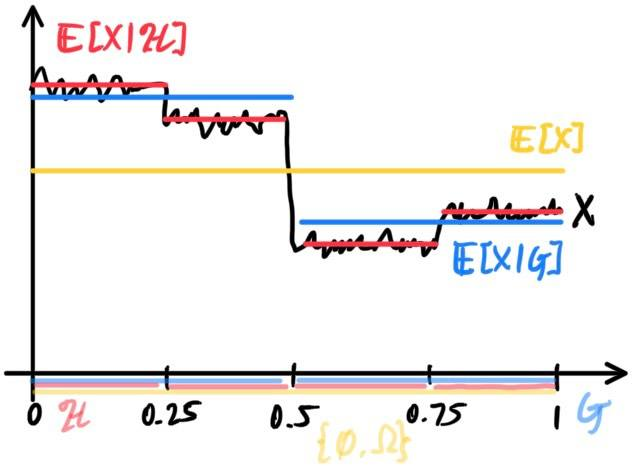
\includegraphics[scale=0.33]{img/function_approximation_conditional.jpg}
\end{center}

Therefore, we can see that if $\mathbb{E}[X \mid \mathcal{G}]$ is $\mathcal{F}$-measurable, then 
\[X = \mathbb{E}[X \mid \mathcal{G}]\]
since its value coincides with $X$ for every event in $\mathcal{F}$. One way to think about it is that $\mathbb{E}[X \mid \mathcal{G}]$ is the conditional expectation of $X$ (which is "detailed" up to resolution $\sigma(\mathcal{G})$) taken with a camera of resolution $\mathcal{G}$. The finer (bigger) the $\sigma$-algebra is, the higher the resolution. 

\subsection{Properties of Conditional Expectation}

\begin{theorem}[Tower Rule]
The expectation of $X$ and its approximation always coincides. 
\[\mathbb{E}[X] = \mathbb{E}[\mathbb{E}[X \mid \mathcal{G}]]\]
\end{theorem}

\begin{lemma}
Let $\mathbb{E}[|X|] , \mathbb{E}[|Y|] < \infty$. Then, 
\begin{enumerate}
    \item Conditional expectation is linear
    \[\mathbb{E}[a X + b Y \mid \mathcal{G}] = a \mathbb{E}[X \mid \mathcal{G}] + b \mathbb{E}[Y \mid \mathcal{G}]\]
    
    \item If $X \leq Y$, then 
    \[\mathbb{E}[X \mid \mathcal{G}] \leq \mathbb{E}[Y \mid \mathcal{G}]\]
\end{enumerate}
\end{lemma}

\begin{theorem}[Jensen's Inequality]
If $\varphi$ is convex and $\mathbb{E}[|X|], \mathbb{E}[|\varphi(X)|] < \infty$, then 
\[\varphi(\mathbb{E}[X \mid \mathcal{G}]) \leq \mathbb{E}[\varphi(X) \mid \mathcal{G}]\]
\end{theorem}

\begin{theorem}
Conditional expectation is a contraction in $L^p$, $p \geq 1$. 
\end{theorem}

\begin{theorem}
If $X$ is $\mathcal{F}$-measurable and $\mathbb{E}[|Y|], \mathbb{E}[|XY|] < \infty$, then 
\[\mathbb{E}[XY \mid \mathcal{F}] = X \mathbb{E}[Y \mid \mathcal{F}]\]
\end{theorem}

\begin{theorem}
Suppose $\mathbb{E}[X^2] < \infty$. Then, $\mathbb{E}[X \mid \mathcal{G}]$ is the $\mathcal{G}$-measurable function $Y$ that minimizes the mean squared error 
\[\mathbb{E}[ (X - Y)^2]\]
\end{theorem}

This gives a nice geometric interpretation of $\mathbb{E}[X \mid \mathcal{G}]$. Given that $X$ lives in the Hilbert space $L^2_\mathcal{F} (\Omega)$, $\mathbb{E}[X \mid \mathcal{G}]$ is the projection of $X$ onto the subspace $L^2_\mathcal{G} (\Omega)$. 
\begin{center}
    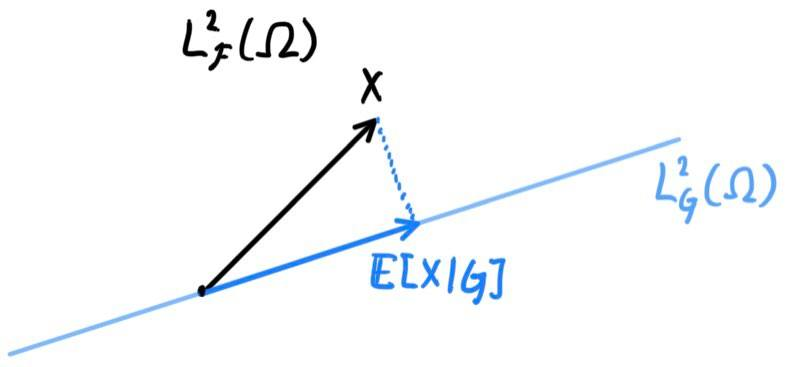
\includegraphics[scale=0.3]{img/Hilbert_Space_projection.jpg}
\end{center}
Therefore, we can change the way think about $\mathbb{E}[X]$. It is not just a value, but rather, we can think of it as our best prediction of $X$ given no information. Specifically, 
\[\mathbb{E}[X] = \mathbb{E}[X \mid \{\emptyset, \Omega\}]\]
That is, letting $\mathcal{G}$ be the trivial $\sigma$-algebra, we must find the best approximation of $X$ that is $\mathcal{G}$-measurable. But any random variable that is $\mathcal{G}$-measurable must be constant, since if we take the preimage of any singleton set $\{x\} \in \mathcal{R}$, then it must be either $\emptyset$ ($X$ does not map to it) or $\Omega$ ($X$ maps all of $\Omega$ to it).

\subsection{Perfect Information vs No Information}

Now let us state some properties on how certain $\sigma$-algebras can change the conditional expectation of certain random variables. 

\begin{theorem}[Perfect Information]
If $X$ is $\mathcal{G}$-measurable, then 
\[\mathbb{E}[X \mid \mathcal{G}] = X\]
That is, the values of $X$ are defined on $\sigma(X) \subset \mathcal{F}$ and so has a detail level of $\sigma(X)$. But if we condition it on an even finer $\mathcal{G} \supset \sigma(X)$, then we are taking a picture of $X$ with something that has overly high resolution, and so our best approximation of $X$ is $X$ itself. Indeed, if $X$ lives in $L_\mathcal{G} (\Omega)$, then its projection onto $L_\mathcal{G} (\Omega)$ is $X$ itself. 
\end{theorem}

\begin{theorem}[Irrelevant Information]
If $X$ is independent of $\mathcal{G}$, i.e. $\sigma(X)$ and $\mathcal{G}$ are independent $\sigma$-algebras, then 
\[\mathbb{E}[X \mid \mathcal{G}] = \mathbb{E}[X]\]
That is, our best approximation of $X$ given information $\mathcal{G}$ is $\mathbb{E}[X]$ itself, i.e. if you don't know anything about $X$, then the best guess is the mean $\mathbb{E}[X]$. To see why, note that independence means that for all $A \in \mathcal{G}$ and $B \in \mathcal{R}$, 
\[\mathbb{P}(X^{-1} (B) \cap A) = \mathbb{P}(X^{-1}(B)) \cdot \mathbb{P}(A)\]
\end{theorem}

\begin{theorem}[Trivial Information]
If $\mathcal{G} = \{\emptyset, \Omega\}$, then 
\[\mathbb{E}[X \mid \mathcal{G}] = \mathbb{E}[X]\]
This makes sense since we're trying to measure $\sigma(X)$-measurable $X$ with the trivial $\mathcal{G}$, and the only function that is measurable w.r.t. the trivial $\sigma$-algebra is a constant function (since the preimage of every Borel set in $\mathcal{R}$ must be either $\Omega$ or $\emptyset$). This is the same as projecting $X$ to the line of constant functions in $L_\mathcal{F}(\Omega)$. 
\end{theorem}

\begin{theorem}
If $\mathcal{F}_1 \subset \mathcal{F}_2$, then 
\begin{enumerate}
    \item $\mathbb{E}[ \mathbb{E}[X \mid \mathcal{F}_1] \mid \mathcal{F}_2] = \mathbb{E}[X \mid \mathcal{F}_1]$. 
    \item $\mathbb{E}[ \mathbb{E}[X \mid \mathcal{F}_2] \mid \mathcal{F}_1] = \mathbb{E}[X \mid \mathcal{F}_1]$. 
\end{enumerate}
In other words, the smaller $\sigma$-algebra always wins. 
\end{theorem}

We can see this visually since in both cases, we are projecting $X$ onto $L^2_{\mathcal{F}_1} (\Omega)$ and onto $L^2_{\mathcal{F}_2} (\Omega)$, but either way, we end up in $L^2_{\mathcal{F}_1} (\Omega)$. Additionally, this is also consistent with our camera analogy, where $\mathbb{E}[X \mid \mathcal{G}]$ is like taking a picture of random variable $X$ with a camera of resolution $\mathcal{G}$. Conditional expectation is essentially an averaging/blurring operator. So, $\mathbb{E}[\mathbb{E}[X \mid \mathcal{G}] \mid \mathcal{H}]$ is like taking a picture of $X$ with resolution $\mathcal{H}$ and then with $\mathcal{G}$. The lower resolution would always win. 

\subsection{Computation of Conditional Expectation}

\begin{definition}
Given probability space $(\Omega, \mathcal{F}, \mathbb{P})$, the conditional expectation of $Y$ given $X$ is the random variable 
\[\mathbb{E}[X \mid Y] \coloneqq \mathbb{E}[X \mid \sigma(Y)]\]
Note that since both $X$ and $Y$ are random variables, they are both $\mathcal{F}$-measurable. However, this doesn't mean that they may be $\mathcal{G}$-measurable for some sub-$\sigma$-algebra $\mathcal{G}$. So, as long as $\sigma(Y) \subset \sigma(X)$ (neither of which may be $\mathcal{F}$), we have some nontrivial approximation. 
\end{definition}

Now let's introduce a new way to think about expectation and conditional expectation in general. 
\begin{enumerate}
    \item The first step is to think of $\mathbb{E}[X]$ not as a value $\mu$ but as the best estimate for the value of a random variable $X$ in the absence of any information. To minimize the squared error 
    \[\mathbb{E}[ (X - e)^2] = \mathbb{E}[ X^2 - 2 e X + e^2] = \mathbb{E}[X^2] - 2 e \mathbb{E}[X] + e^2\]
    we differentiate with respect to $e$ to obtain $2e - 2 \mathbb{E}[X] = 0 \implies e = \mathbb{E}[X]$. For example, if I throw a fair die and you have to estimate its value $X$, according to the analysis above, your best bet is to guess $\mathbb{E}[X] = 3.5$ since $\Omega = \{1, 2, 3, 4, 5, 6\}$. On specific rolls of the die, this will be an over-estimate of an underestimate, but on the long run it minimizes the mean square error. 
    
    \item If we \textit{do} have additional information, then we use conditional expectation. Suppose that I tell you that $X$ is an even number. Then, I would guess that the possible values of $X$ are $\{2, 4, 6\}$, and so the our conditional expectation is $4$. Similarly, if I told you that $X$ is odd, then the conditional expectation is $3$. This additional information can be put into a random variable $Y: \Omega \rightarrow \mathbb{R}$ defined 
    \[Y(\omega) = \begin{cases} 0 & \text{ if } \omega = 2, 4, 6 \\ 1 & \text{ if } \omega = 1, 3, 5 \end{cases}\]
    Then, we can say that $\mathbb{E}[X \mid Y = 0] = 4$ and $\mathbb{E}[X \mid Y = 1] = 3$. We can interpret this as the conditional expectation given the $\sigma$-algebra generated by these two sets $\{2, 4, 6\}$ and $\{1, 3, 5\}$. 
    
    \item Now, imagine that I roll the die and I tell you the parity of $X$. You should see that a single numerical response cannot cover both cases. You would respond $3$ if I tell you $X$ is odd ($Y = 1$) and $4$ if I tell you $X$ is even ($Y = 0$). A single numerical response is not enough because the particular piece of information I give you is \textit{itself random}. In fact, your response is necessarily a function of this particular piece of information, represented in our notation as 
    \[g(Y) = \mathbb{E}[X \mid Y] = \begin{cases} 3 & \text{ if } Y = 1 \\ 4 & \text{ if } Y = 0 \end{cases}\]
    This is a function of $Y$, and it is consistent with our understanding of $\mathbb{E}[X \mid Y]$ as our "best estimate" of $X$ with random variable $Y$. 
    \begin{center}
        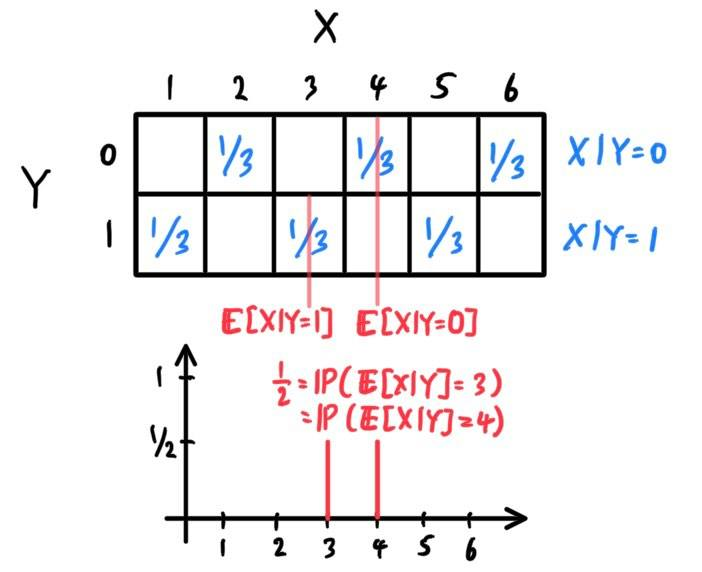
\includegraphics[scale=0.3]{img/conditional_expect_dice.jpg}
    \end{center}
\end{enumerate}

From the visual above, we can see that we take the joint distribution $X \times Y$, and for each value $Y = y$, we can estimate $X$ as $\mathbb{E}[X \mid Y = y]$. But now there is the additional uncertainty of what value $Y$ will take, which turns this value estimate $\mathbb{E}[X \mid Y = y]$ in a distribution $\mathbb{E}[X \mid Y]$. So, for the discrete case, 
\[\mathbb{P}\big( \mathbb{E}[X \mid Y] = \mathbb{E}[X \mid Y = y]) = \mathbb{P}(Y = y)\]

Now we can talk about how to compute conditional expectation. In essence, the conditional expectation $\mathbb{E}[X \mid Y]$ is simply a function of a random variable $Y$ that is this best approximation. Given a joint random variable $(X, Y): \Omega \rightarrow \mathbb{R}^2$, we can fix a value of $Y = y$. Therefore, we are given the information that event $Y^{-1}(\{y\})$ happened, and so we can construct our conditional distribution $X \mid Y = y$, which defines a new probability measure. Taking the expectation of that gives us a number. 


\begin{definition}[Discrete Conditional Expectation Given $Y = y$]
Let $X, Y$ be discrete random variables, with joint random variable $(X, Y): \Omega \rightarrow \mathbb{R}^2$ and its joint PMF $p_{X, Y} (x, y)$. Recall that the conditional PMF is 
\[p_{X\mid Y}(x \mid y) \coloneqq \frac{p_{X, Y} (x, y)}{p_Y (y)}\]
The \textbf{conditional expectation} of $X$ given $Y = y$ is 
\[\mathbb{E}[X \mid Y = y] = \sum_{x \in \mathcal{X}} x \, p_{X \mid Y} (x \mid y)\]
\end{definition}

\begin{definition}[Continuous Conditional Expectation Given $Y = y$]
Let $X, Y$ be jointly continuous with joint PDF $f_{X, Y} (x, y)$. Recall that the conditional PDF is 
\[f_{X \mid Y} (x \mid y) \coloneqq \frac{f_{X, Y} (x, y)}{f_Y (y)}\]
The \textbf{conditional expectation} of $X$ given $Y = y$ is 
\[\mathbb{E}[X \mid Y = y] = \int_{x \in \mathbb{R}} x \, f_{X \mid Y} (x \mid y) \, dx\]
Again, we can set $\psi(y) \coloneqq \mathbb{E}[X \mid Y = y]$, which is a function of $y$ and therefore a random variable. 
\end{definition}

As a visual, we can take a "slice" of the joint distribution of some value of $Y$, look at the distribution of $X$ on this slice, and compute its expectation. That is, for every value of $Y = y$, there exists some (conditional) distribution of $X$ with PMF of $p_{X \mid Y} (x \mid y)$ or PDF of $f_{X \mid Y} (x \mid y)$. 
\begin{center}
    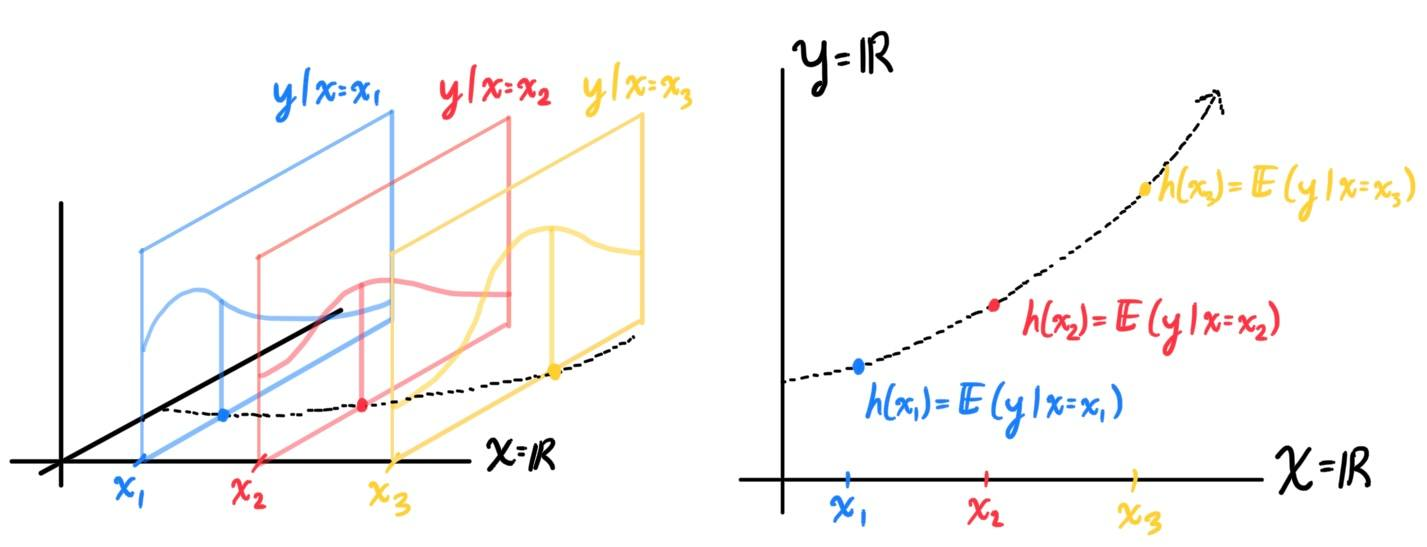
\includegraphics[scale=0.3]{img/conditional_exp.jpg}
\end{center}
So given a value of $Y = y$, we generally know something about $X$ (e.g. if I know humidity, I know something about the temperature) and want to find the best estimate of $X$. This is precisely the conditional expectation $\mathbb{E}[X \mid Y = y]$, and we can interpret this as a regression function $\psi(y) \coloneqq \mathbb{E}[X \mid Y = y]$, which predicts the expected value of $X$ given $Y = y$. 

But since we don't know what exactly $Y$ is, this process is random itself, and it is only after this $Y$ is realized that we can provide the expected value of $X$. Thus, by replacing the little $y$'s with the big $Y$'s, we can construct a random variable that will estimate $X$ for us given $Y$, denoted $\mathbb{E}[X \mid Y] = \psi(Y)$. This turns out to be a $\sigma(Y)$-measurable random variable itself. 

\begin{example}
Let $f_{X, Y} (x, y) = \frac{1}{x}$ for $0 < y \leq x \leq 1$. Find $\mathbb{E}[Y \mid X]$. We first calculate the marginal density of $X$, which will allow us to calculate the conditional density of $Y$: 
\[f_X (x) = \int_0^x \frac{1}{x} \,dy = \frac{y}{x} \bigg|_0^x = 1 \implies f_{Y \mid X} (y \mid x) = \frac{f_{X, Y} (x, y)}{f_X (x)} = \frac{1/x}{1} = \frac{1}{x} \text{ for } 0 < y \leq x \leq 1\]
Since the conditional density of $Y$ is not dependent on $x$, $Y$ is uniform from $0$ to $x$. Now calculate the expectation: 
\[\mathbb{E}[Y \mid X = x] = \int_0^x y \cdot \frac{1}{x} \,dy = \frac{x}{2}\]
and so the conditional expectation is 
\[\mathbb{E}[Y \mid X] = \frac{1}{2} X\]
\end{example}

A fundamental result in statistical learning theory is that if we have two random variables $X$ and $Y$, the best predictor of $Y$ as a function of $X$ is the conditional expectation $\mathbb{E}[Y \mid X]$. 

\begin{theorem}
Let us have two random variables $X$ and $Y$, with $g(X) = \mathbb{E}[Y \mid X]$. Then, the function $g$ minimizes the cost function $\mathbb{E}[ (Y - h(X))^2]$. That is, 
\[\inf_{h \text{ meas.}} \mathbb{E}[( Y - h(X))^2] = \mathbb{E} [(Y - g(X))^2]\]
\end{theorem}

We restate the tower rule again. 

\begin{theorem}[Tower Rule]
We know that $\mathbb{E}[Y \mid X]$ is the random variable $\psi(X)$ that is a transformed version of $X$. Then, we have
\[\mathbb{E}[ \mathbb{E}[Y \mid X]] = \mathbb{E}[Y]\]
This is confusing notation due to the iterated expectations, but note that the term on the inside is a transformed random variable of $X$, while the expectation on the outside computes the expectation of this transformed random variable. So, letting $\psi(X) = \mathbb{E}[Y \mid X]$, we can equivalently write 
\[\mathbb{E}[ \psi(X)] = \mathbb{E}[Y]\]
Intuitively, this makes sense, since $\mathbb{E}[Y \mid X]$ is the random variable that tries to "model" $Y$ given (random) information from $X$, so its expectation must be the expectation of $Y$ itself. 
\end{theorem}
\begin{proof}
We can just expand this out. We will do it for the discrete case. 
\begin{align*}
    \mathbb{E}[ \mathbb{E}[Y \mid X]] & = \sum_x p_X (x) \, \underbrace{\mathbb{E}[Y \mid X = x]}_{\psi(x)} \\
    & = \sum_x \bigg( p_X (x) \cdot \sum_y y \cdot p_{Y \mid X} (y \mid x) \bigg) \\
    & = \sum_x \bigg( p_X (x) \cdot \sum_y y \cdot \frac{p_{X, Y} (x, y)}{p_X (x)} \\
    & = \sum_{x, y} y \cdot p_{X, Y} (x, y) \\
    & = \sum_y \bigg( y \cdot \sum_x p_{X, Y} (x, y) \bigg) \\
    & = \sum_y y \cdot p_Y (y) \\
    & = \mathbb{E}[Y]
\end{align*}
\end{proof}

\begin{example}
Consider the random sum of random variables $S_N = \sum_{i=1}^N X_i$, where $X_i$ are iid and $N$ is independent of $X_i$'s. Then, we can use the tower rule to write $\mathbb{E}[S_N] = \mathbb{E}[\mathbb{E}[S_N \mid N]]$. $\mathbb{E}[S_N \mid N]$ is a transformed random varibale of $N$, and to compute its closed form we should just compute $\mathbb{E}[S_N \mid N = n]$ and replace $n$ with $N$. 
\[\mathbb{E}[S_N \mid N = n] = \mathbb{E}[S_n] = \mathbb{E} \bigg( \sum_{i=1}^n X_i \bigg) = n \mathbb{E}[X]\]
remember that $\mathbb{E}[X]$ is just a number, so replacing $n$ with $N$ gives $\mathbb{E}[S_N \mid N] = N \mathbb{E}[X]$, i.e. the random variable $N$ multiplied by $\mathbb{E}[X]$. Therefore, 
\[\mathbb{E}[\mathbb{E}[S_N \mid N]] = \mathbb{E}[N \mathbb{E}[X]] = \mathbb{E}[N] \, \mathbb{E}[X]\]
This makes sense intuitively, since we want to approximate this value by taking the expected value of $X$ and multiplying it by the expected number of summands. 
\end{example}

Now, we can simply use the property to talk about what $\mathbb{P}(X \mid Y)$ means. Formally, using the fact that the probability that $X$ will realize in $A$, i.e. $\mathbb{P}(X \in A) = \mathbb{E}_X[1_A]$, we can define the conditional probability as 
\[\mathbb{P}(X \in A \mid Y) = \mathbb{E}[ 1_X \mid Y] \]
We can interpret this in multiple ways, in increasing level of rigor. Let $(\Omega, \mathcal{F}, \mathbb{P})$ be a probability space, with random variables $X, Y$ with their probability laws $\mathbb{P}_X, \mathbb{P}_Y$. 
\begin{enumerate}
    \item When $Y$ realizes, we can use this definition to have a better educated guess of where $X$ will land. But since $Y$ is random, so is our guess. 
    
    \item Let us have the joint distribution $(X, Y)$. Given that $Y = y$, we can take the conditional distribution $X \mid Y = y$ and compute the event that this random variable lands in $A$ by replacing the little $y$'s with the big $Y$'s. 
    
    \item Let $A$ be an event in $\mathcal{R}$. Then, the probability that $X$ will land in $A$ is 
    \[\mathbb{P}(X \in A) = \mathbb{P}_X(A) = \mathbb{P}(X^{-1} (A))\]
    where the first is abuse of notation, the second is the probability law of $\mathbb{R}$, and the third is the probability law of $\Omega$. Then, $1_A$ generates a $\sigma$-algebra $\sigma(1_A)$ on $\Omega$, consisting of the sets $\{\emptyset, X^{-1}(A), X^{-1}(A)^c, \Omega\}$. 
\end{enumerate}

\subsection{Conditional Expectation given Multiple Random Variables}

Now the $\sigma$-algebra generated by multiple random variables should intuitively be bigger than the $\sigma$-algebra generated by one random variable. We can't simply take the union of the individual $\sigma$-algebras. 

\begin{definition}[$\sigma$-algebra generated by Multiple Random Variables]
Given random variables $\{X_i\}_{i \in I}$ indexed by some set (possibly uncountable), the $\sigma$-algebra generated by this collection is defined 
\[\sigma(X_1, \ldots, X_n) \coloneqq \sigma \bigg( \bigcup_{i \in I} \sigma(X_i) \bigg) \]
\end{definition}

Let us look at $\mathbb{E}[X \mid Y, Z]$ and compare it to $\mathbb{E}[X \mid Y]$. From this definition, we know that the information about $X$ contained in $\sigma(Y, Z)$ is at least as great as the corresponding information in $\sigma(Y)$. Therefore, we can simply define conditional expectation as such: 

\begin{definition}[Conditional Expectation given Multiple Random Variables]
Given random variables $\{X_i\}_{i \in I}$, the conditional expectation is defined 
\[\mathbb{E}[Y \mid \{X_i\}_{i \in I} ] = \mathbb{E}[ Y \mid \sigma(\{X_i \}_{i \in I} ]\]
which is the random variable where 
\[\int_A Y \, d\mathbb{P} = \int_A \mathbb{E}[Y \mid \{X_i\}_{i \in I} ] \, d\mathbb{P}\]
for all $A \in \sigma(\{X_i \}_{i \in I})$. 
\end{definition}

\subsection{Conditional Variance}

Similar to conditional expectation, we can define the conditional variance $\mathrm{Var}(Y \mid X = x)$ as a function $h(x)$ that outputs the variance of $Y$ given $X = x$. We have
\begin{align*}
    \mathrm{Var}(Y \mid X = x) & = \mathbb{E}\big[ ( Y - \mathbb{E}[Y \mid X = x] )^2 \mid X = x \big]
\end{align*}

\begin{definition}[Conditional Variance]
The \textbf{conditional variance} of $Y$ given $X$ is defined as 
\[\Var(Y \mid X) = \mathbb{E} \big[ \big( Y - \mathbb{E}[Y \mid X] \big)^2 \mid X \big] \]
which tells us how much variance is left if we use $\mathbb{E}[Y \mid X]$ to predict $Y$. 
\end{definition}





\section{Common Distributions}

\subsection{Multivariate Gaussians}

Recall $X \sim \mathcal{N}(\mu, \sigma^2)$ implies that its PDF is 
\[f_X (x) = \frac{1}{\sigma \sqrt{2 \pi}} e^{-\frac{(x - \mu)^2}{2 \sigma^2}}\]
Now we will consider a Gaussian random \textit{vector}, which can be considered a vector of random variables  
\[\mathbf{X} = \begin{bmatrix} X_1 \\ X_2 \\ \vdots \\ X_n \end{bmatrix}\]
mapping from $\Omega$ to $\mathbb{R}^n$. It is not merely a vector where every $X_i$ is Gaussian, as we will show later. That is, a joint distribution that has all $n$ marginal distributions Gaussians does not make a multivariate Gaussian. 

This measurable function $\mathbf{X}: \Omega \rightarrow \mathbb{R}^n$ induces a probability law $\mathbb{P}_X$ on $\mathcal{B}(\mathbb{R}^n)$, and the Radon-Nikodym theorem states the existence of a PDF $f_X$ such that $\mathbb{P}_X (B) = \int_B f_X \,d\lambda$.

\subsubsection{Bivariate Gaussians}
Let us first begin with two-variable Gaussians. 

\begin{definition}[Standard Bivariate Gaussian RV]
A random variable $(X, Y)$ is said to be a \textbf{standard bivariate Gaussian} if its PDF is of form
\[f_{X, Y} (x, y) = \frac{1}{2 \pi \sqrt{1 - \rho^2}} \exp \bigg( -\frac{x^2 - 2 \rho x y + y^2}{2 (1 - \rho^2)} \bigg) \text{ for } \rho \in (-1, 1)\] 
\end{definition}

\begin{proposition}
Given a standard bivariate Gaussian $(X, Y)$, 
\begin{enumerate}
    \item $X$ and $Y$ are marginally distributed as $\mathcal{N}(0, 1)$. That is, if we integrate a variable (say, $x$) out, we will get a univariate standard Gaussian PDF of the other ($y$): 
    \[\int_{-\infty}^\infty \frac{1}{2 \pi \sqrt{1 - \rho^2}} \exp \bigg( -\frac{x^2 - 2 \rho x y + y^2}{2 (1 - \rho^2)}\bigg) \,dx = \frac{1}{\sqrt{2 \pi}} e^{-y^2 / 2}\]
    \item $\rho_{X, Y}$, the correlation coefficient of $X$ and $Y$, is equal to $\rho$. 
    \item The conditional distribution of $X$ given $Y = y$ is $X \mid Y = y \sim \mathcal{N} (\rho y, 1 - \rho^2)$. That is, 
    \[f_{X \mid Y} (x \mid y) = \frac{1}{2 \pi \sqrt{1 - \rho^2}} \exp \bigg( -\frac{x^2 - 2 \rho x y + y^2}{2 (1 - \rho^2)}\bigg) = \frac{1}{ \sqrt{2 \pi (1 - \rho^2)}} \, \exp\bigg( - \frac{(x - (\rho y))^2}{2 (1 - \rho^2)} \bigg)\]
    \item From (3), we can see that the conditional expectation $\mathbb{E}[X \mid Y = y] = \rho y$ since $X \mid Y = y$ has mean at $\rho y$. Therefore, the conditional expectation of $X$ given $Y$ (which is a random variable) is 
    \[\mathbb{E}[X \mid Y] = \rho Y\]
    i.e. $\mathbb{E}[X \mid Y]$ is a linear function of $Y$. 
\end{enumerate}
\end{proposition}

The formula of the general bivariate Gaussian $\mathbf{X} = (X_1, X_2)$ PDF is messy, but we will put it here. 
\[f_{X_1, X_2} (x, y) = \frac{\sigma_1 \sigma_2 \sqrt{1 - \rho^2}} \exp \bigg[ -\frac{1}{2} \bigg( \frac{(x_1 - \mu_1)^2}{\sigma_1^2} + \frac{(x_2 - \mu_2)^2}{\sigma_2^2} - 2 \rho \frac{(x_1 - \mu_1)}{\sigma_1} \frac{(x_2 - \mu_2)}{\sigma_2}\bigg)\bigg]\]
It is cleaner to put it into matrix form. 
\[f_{X_1, X_2} (x_1 , x_2) = \frac{1}{2 \pi \sqrt{\mathrm{det}(\boldsymbol{\Sigma})}} \exp \bigg( - \frac{(\mathbf{x} - \boldsymbol{\mu})^T \boldsymbol{\Sigma}^{-1} (\mathbf{x} - \boldsymbol{\mu})}{2} \bigg) \]
where 
\[\mathbf{x} = \begin{pmatrix} x_1 \\ x_2 \end{pmatrix}, \;\; \boldsymbol{\mu} = \begin{pmatrix} \mu_1 \\ mu_2 \end{pmatrix} , \;\; \boldsymbol{\Sigma} = \mathbb{E}\big[ (\mathbf{X} - \boldsymbol{\mu}) (\mathbf{X} - \boldsymbol{\mu})^T \big] = \begin{pmatrix} \mathrm{Var}(X_1) & \mathrm{Cov}(X_1, X_2) \\
\mathrm{Cov}(X_1, X_2) & \mathrm{Var}(X_2) \end{pmatrix}\]

Note that visually, $\boldsymbol{\Sigma}$ will determine how much the Gaussian distribution is "stretched" on one way or another. Obviously, the "peak" of the distribution will be $\boldsymbol{\mu}$. If $\boldsymbol{\Sigma} = I$, then we could visualize the Gaussian distribution as being perfectly symmetric. However, if we scale the distribution up to a certain constant (below shown $\boldsymbol{\Sigma} = I$, $\boldsymbol{\Sigma} = 0.61 I$, $\boldsymbol{\Sigma} = 2 I$), we get
\begin{center}
    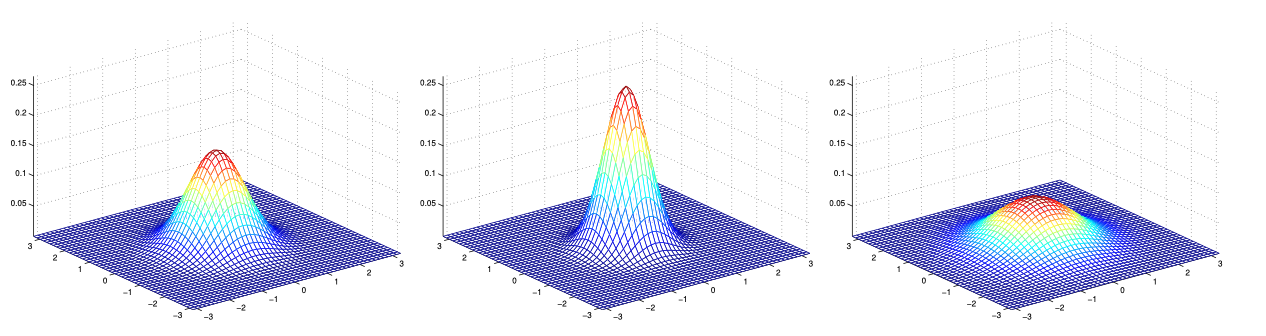
\includegraphics[scale=0.65]{img/Gaussian_Distribution.png}
\end{center}

Now we've made a remark before that given a multivariate distribution $\mathbf{X} = (X_1, \ldots, X_n)$, all of its marginal distributions being Gaussian does not mean that $\mathbf{X}$ is a multivariate Gaussian. We give a counterexample. 

\begin{example}
Let $Y_1, Y_2$ be iid random variables distributed according to the PDF 
\[f_Y (y) = \sqrt{\frac{2}{\pi}} e^{-y^2 / 2} \text{ for } y > 0\]
which we can interpret as a one-sided Gaussian. Let $W \sim \mathrm{Bernoulli}(\frac{1}{2})$ be independent of $Y_1$ and $Y_2$. Now, define the random variables 
\[X_1 = W \, Y_1 \text{ and } X_2 = W \, Y_2\]
Now note that $Y_1$ and $Y_2$ are both positive, and since $X_1$ and $X_2$ are both dependent on the same value of $W$, it is either $X_1$ and $X_2$ are both positive or both negative. So, the joint distribution of $X_1, X_2$ will be on only the 1st and 3rd quadrant with no mass on the 2nd and 4th. 
\begin{center}
    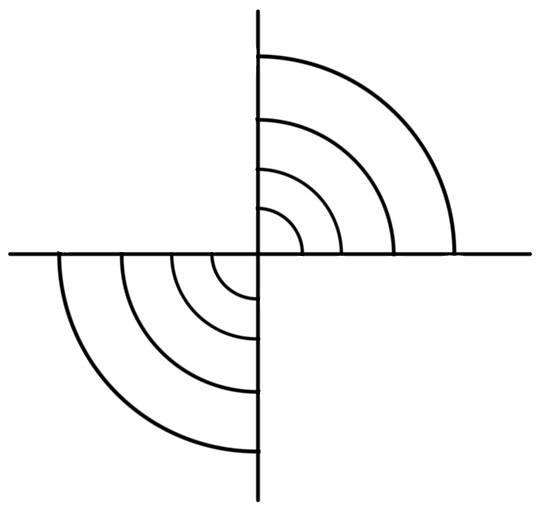
\includegraphics[scale=0.23]{img/not_multi_Gaussian.jpg}
\end{center}
This is clearly not a multivariate Gaussian, even though the marginals are $X_1, X_2 \sim \mathcal{N}(0, 1)$. We could make the degenerate case that $X_1 = X_2$, which would make the image of $(X_1, X_2)$ just the line at $x_1 = x_2$, but we can think of this as a degenerate Gaussian with a singular $\boldsymbol{\Sigma}$. 
\end{example}

\subsubsection{Multivariate Gaussians}

There are three equivalent definitions of multivariate Gaussians of $n$-variables. 

\begin{definition}[Multivariate Gaussian]
Let us have a vector-valued random variable $\mathbf{X} = (X_1 \ldots X_n)^T \sim \mathcal{N}(\boldsymbol{\mu}, \boldsymbol{\Sigma})$. 
\begin{enumerate}
    \item $\mathbf{X}$ is a \textbf{multivariate Gaussian distribution} with mean $\boldsymbol{\mu} \in \mathbb{R}^n$ and symmetric, positive-definite covariance matrix $\boldsymbol{\Sigma} \in \mathbb{R}^{n \times n}$ if its probability density function is
    \[f_X (x) = \frac{1}{(2\pi)^{n/2} \mathrm{det}(\boldsymbol{\Sigma})^{1/2}} \exp\bigg( -\frac{1}{2} (x-\boldsymbol{\mu})^T \boldsymbol{\Sigma}^{-1} (x - \boldsymbol{\mu})\bigg)\]
    The covariance matrix $\boldsymbol{\Sigma}$ is the $n \times n$ matrix whose $(i, j)$th entry is $\Cov(X_i, X_j)$. That is, for any random vector $\mathbf{X}$ with mean $\boldsymbol{\mu}$, its covariance matrix 
    \[\boldsymbol{\Sigma} = \mathbb{E}\big[ (\mathbf{X} - \boldsymbol{\mu}) (\mathbf{X} - \boldsymbol{\mu})^T \big] = \mathbb{E}[\mathbf{X} \mathbf{X}^T] - \boldsymbol{\mu} \boldsymbol{\mu}^T\]
    is positive definite and symmetric, which implies by the spectral theorem we can break it down into $n$ orthogonal eigenspaces of positive eigenvalues. 

    \item $X$ is a multivariate Gaussian distribution if it can be expressed as 
    \[\mathbf{X} = \mathbf{D} \mathbf{w} + \boldsymbol{\mu}\]
    where $\mathbf{w}$ is a vector of independent $\mathcal{N}(0, 1)$ Gaussians, $\boldsymbol{\mu} \in \mathbb{R}^n$, and $\mathbf{D} \in \mathbb{R}^{n \times n}$. The mean of $\mathbf{X}$ is $\boldsymbol{\mu}$ and its covariance is $\boldsymbol{\Sigma} = \mathbf{D} \mathbf{D}^T$; $\mathbf{D}$ is called the \textbf{standard deviation matrix}. When modeling high-dimensional Gaussians, this way is most computationally feasible. 

    \item $X$ is a multivariate Gaussian distribution if for every $\mathbf{a} \in \mathbb{R}^n$, $\mathbf{a}^T \mathbf{x}$ is a Gaussian RV. This means that if we take $\mathbf{a} = \mathbf{0}$, then the entire $\mathbf{X}$ is constantly $0$, which we will take to be the degenerate Gaussian with mean, variance $0$. 
\end{enumerate}
The $n$ semi-axes of the $(n-1)$-dimensional isocontour ellipsoid formed by an $n$-dimensional Gaussian distribution are precisely the normalized eigenvectors of $\boldsymbol{\Sigma}$ multiplied by their eigenvalues. 
\end{definition}


If we let $\boldsymbol{\Sigma} = \mathbf{I}$, then this means that all the $X_i$'s are pairwise uncorrelated since $\Sigma_{ij} = \Cov (X_i, X_j) = 0$. In general, this does not mean that the $X_i$'s are independent, but for joint Gaussians, this also implies independence! 

\begin{theorem}
Given multivariate Gaussian $\mathbf{X} = (X_1 \ldots X_n)^T \sim \mathcal{N}(\boldsymbol{\mu}, \boldsymbol{\Sigma})$, the $X_i$'s are pairwise independent if and only if they are uncorrelated. 
\end{theorem}
\begin{proof}
We can expand the PDF of $\mathbf{X}$ as 
\begin{align*}
    f_X (x) & = \frac{1}{(2 \pi)^{n/2}} \exp \bigg( -\frac{1}{2} (x - \mu)^T (x - \mu) \bigg) \\
    & = \bigg(\frac{1}{\sqrt{2\pi}} \bigg)^n \exp \bigg( \sum_{i=1}^n -\frac{1}{2} (x_i - \mu_i)^2 \bigg) \\
    & = \prod_{i=1}^n \frac{1}{\sqrt{2\pi}} \exp \bigg( -\frac{1}{2} (x_i - \mu_i)^2 \bigg)
\end{align*}
which is the product of $n$ single-variable Gaussians $X_i$. Therefore this means that independence and uncorrelation are equivalent! 
\end{proof}

Therefore, if the nondiagonal entries of the covariance matrix are all $0$, then we know that the variables are all uncorrelated and therefore independent. 

\end{document}

